\documentclass[a4paper,twoside]{book}
\usepackage[italian]{babel}
\usepackage[utf8]{inputenc}
\usepackage{amsmath}
\usepackage{amsthm}
\usepackage{amsfonts}
\usepackage{amssymb}
\usepackage{cancel}
\usepackage[margin=1in]{geometry}
\usepackage{hyperref}
\usepackage{graphicx}
\usepackage{wrapfig}
\usepackage{listings}
\usepackage{algorithm}
\usepackage[noend]{algpseudocode}
\usepackage{fancyhdr}
\usepackage{wrapfig}
\usepackage{nicematrix}
\usepackage{soul}
\usepackage{tikz}
\usepackage{subcaption}

\graphicspath{{./images/}}

\makeatletter
\newenvironment{abstract}{%
    \if@twocolumn
        \section*{\abstractname}%
    \else
        \begin{center}%
            {\bfseries \abstractname\vspace{-.5em}\vspace{\z@}}%
        \end{center}%
        \small
        \begin{quotation}
    \fi}
    {\if@twocolumn\else\end{quotation}\fi}
\makeatother

% Definizione di nuovi comandi per definizioni, caso base e passo induttivo e teoremi
\theoremstyle{definition}
\newtheorem{definition}{Definizione}[chapter]
\newtheorem*{basecase}{Caso Base}
\newtheorem*{inductivecase}{Passo Induttivo}
\newtheorem*{inductiveipothesis}{Ipotesi Induttiva}
\newtheorem{theorem}{Teorema}[chapter]
\newtheorem{example}{Esempio}[chapter]


% Definizione per il package algorithm
\algnewcommand\New{\textbf{new}\ }
\algnewcommand\Nil{\textbf{nil}\ }
\algnewcommand\Print{\textbf{print}\ }
% Definizioni di int, boolean, float
\algnewcommand\Int{\textbf{int}\ }
\algnewcommand\Bool{\textbf{boolean}\ }
\algnewcommand\Float{\textbf{float}\ }
\algnewcommand\To{\textbf{to}\ }
\algnewcommand\DownTo{\textbf{downto}\ }
\algnewcommand\True{\textbf{true}\ }
\algnewcommand\False{\textbf{false}\ }
\algnewcommand\Not{\textbf{not}\ }
\algnewcommand\Or{\textbf{or}\ }
% Definizione di Tree API
\algnewcommand\Tree{\textsc{Tree}\ }
\algnewcommand\Item{\textsc{Item}\ }
\algnewcommand\Queue{\textsc{Queue}\ }
\algnewcommand\PriorityQueue{\textsc{PriorityQueue}\ }
% Grafi
\algnewcommand\Graph{\textsc{Graph}\ }
\algnewcommand\Node{\textsc{Node}\ }
% SET
\algnewcommand\Set{\textsc{Set}\ }
\algnewcommand\List{\textsc{List}\ }
% Altro utile
\algnewcommand\algorithmicforeach{\textbf{foreach}}
\algdef{S}[FOR]{ForEach}[1]{\algorithmicforeach\ #1\ \algorithmicdo}
\algnewcommand\Stack{\textsc{Stack}\ }
\algnewcommand\Deleted{\textsc{deleted}\ }
% Definizione di header e footer

\title{Appunti di Algoritmi e Strutture Dati}
\author{Luca Facchini (mat. 245965)}
\date{A.A. 2024/2025}



\fancypagestyle{chapterInit}{
    \fancyhf{}
    \fancyhead{}
    \fancyfoot{}
    \renewcommand{\headrulewidth}{0pt}
    \renewcommand{\footrulewidth}{0.4pt}
    \fancyfoot[LO,RE]{\thepage}
    \fancyfoot[LE,RO]{``Appunti di Algoritmi e Strutture Dati" di Luca Facchini}
}
\fancypagestyle{stdPage}{
    \fancyhead{}
    \fancyhead[LO]{\leftmark}
    \fancyhead[RE]{\rightmark}
    \fancyfoot{}
    \renewcommand{\footrulewidth}{0.4pt}
    \renewcommand{\headrulewidth}{0.4pt}
    \fancyfoot[LO,RE]{\thepage}
    \fancyfoot[LE,RO]{``Appunti di Algoritmi e Strutture Dati" di Luca Facchini}
}
\fancypagestyle{tocStyle}{
    \fancyhf{}
    \renewcommand{\footrulewidth}{0.4pt}
    \renewcommand{\headrulewidth}{0pt}
    \fancyfoot[LE,RO]{\thepage}
    \fancyfoot[LO,RE]{``Appunti di Algoritmi e Strutture Dati" di Luca Facchini}
}
\fancypagestyle{plain}{
    \thispagestyle{chapterInit}
}

\begin{document}
    \pagenumbering{Roman}
    \begin{titlepage}
        \centering  % Center everything on the title page
        {\Huge\textbf{Appunti di Algoritmi e Strutture Dati}} \\[1cm] % Title
        \vspace{0.5cm}
        
        {\Large Luca Facchini} \\ % Author name
        \vspace{0.3cm}
        {\large Matricola: 245965} \\[2cm] % Additional author info
        
        {\large Corso tenuto dal prof. Montresor Alberto} \\[0.3cm] % Course information
        {\large Università degli Studi di Trento} \\[1.5cm]
        
        {\large A.A. 2024/2025} \\[3cm] % Academic year
        
        % Abstract section with spacing control
        \vfill
        \begin{abstract}
            Appunti del corso di Algoritmi e Strutture Dati tenuto dal prof. Montresor Alberto presso l'Università degli Studi di Trento nell'anno accademico 2024/2025.
        \end{abstract}
        \footnote{Le immagini e gli algoritmi (identificati da Algorithm \#\#) presenti in questo documento sono stati presi dai materiali forniti dal professor Montresor Alberto (\href{mailto:alberto.montresor@unitn.it}{alberto.montresor@unitn.it}) durante il corso, sono condivisi sotto licenza Creative Commons Attribution-ShareAlike 4.0 International License (\href{https://creativecommons.org/licenses/by-sa/4.0/}{CC BY-SA 4.0}). Come conseguenza le sole immagini sono soggette a questa licenza, il contenuto testuale in quanto appunti personali tratti da lezioni ed altro è soggetto alla licenza "genitore" del quale questo documento fa parte}
        
        \vfill  % Pushes the content to the center vertically
    \end{titlepage}
    \newpage
    \pagestyle{tocStyle}
    \renewcommand{\headheight}{14.5pt}
    \begingroup
        \tableofcontents
        \thispagestyle{tocStyle}
    \endgroup
    \newpage
    \pagestyle{stdPage}
    \pagenumbering{arabic}
    \part{Primo Semestre}
    \chapter{Analisi di Algoritmi}
\thispagestyle{chapterInit}
\section{Modelli di calcolo}
    \subsection{Definizioni}    
        \subsubsection{Complessità}
            \begin{definition}
                La \textbf{complessità} di un algoritmo è definita come la quantità di \textbf{tempo} necessaria per eseguirlo in funzione della \textbf{dimensione dell'input}.
            \end{definition}
            Le domande spontanee che ci si pone sono dunque:
            \begin{itemize}
                \item Come definire la dimensione dell'input?
                \item Come misurare il tempo?
            \end{itemize}
        \subsubsection{Dimensione dell'input}
            \begin{definition}
                Per definire la \textbf{dimensione dell'input} abbiamo due criteri:
                \begin{description}
                    \item[Costo Logaritmico] Il costo logaritmico è definito come il numero di bit necessari per rappresentare l'input.
                    \item[Costo Uniforme] La taglia dell'input è definita come il numero di elementi da cui è composto. 
                \end{description}
            \end{definition}
            Ma in molti casi possiamo assumere che tutti gli elementi siano rappresentati dallo stesso numero di bit costante e che coincidono a meno di costante moltiplicativa
        \subsubsection{Tempo}
            \begin{definition} 
                Un'istruzione si considera elementare se può essere eseguita in tempo "costante" dal processore, dunque un esempio ne è la moltiplicazione o una funzione matematica ad esempio $\cos(d)$, ma una istruzione come il massimo tra due numeri non è elementare.
            \end{definition}
        \subsubsection{Modello di calcolo}
            \begin{definition}
                Un modello di calcolo è definito come la rappresentazione astratta di un calcolatore che rispetta i seguenti criteri:
                \begin{description}
                    \item[Astrazione] Il modello deve permettere di nascondere i dettagli.
                    \item[Realismo] Il modello deve riflettere una situazione reale.
                    \item[Potenza Matematica] Il modello deve permettere di dimostrare "formalmente" la complessità di un algoritmo.    
                \end{description}
            \end{definition}
            Esempio di modello di calcolo è la \textbf{Macchina di Turing}.
    \subsection{Esempi di Analisi}
        \subsubsection{Tempo di calcolo $\min()$}
            Sappiamo che ogni istruzione richiede un tempo costante per essere eseguita e che ogni operazione potenzialmente ha una costante diversa dalle altre e che ogni istruzione viene eseguita un numero di volte diversa dalle altre.
            
            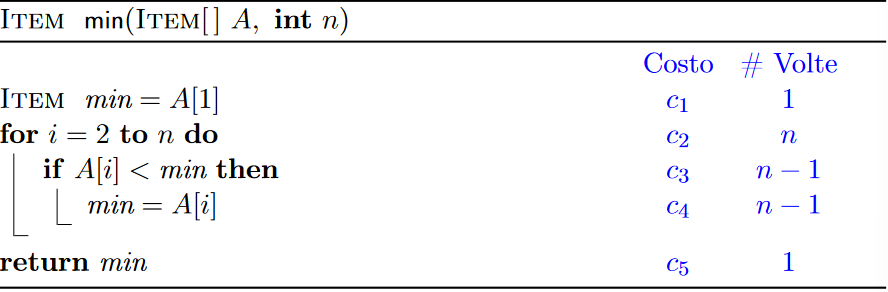
\includegraphics[width=0.9\textwidth]{01/calcoloMin.png}
            
            Otteniamo quindi che il tempo di calcolo è:
            \[
                \begin{aligned}
                    T(n)=&c_1+c_2n+c_3(n-1)+c_4(n-1)+c_5\\
                    =&(c_2+c_3+c_4)n+(c_1+c_5-c_3-c_4) = an+b
                \end{aligned}
            \]
        \subsubsection{Tempo di calcolo di $\operatorname{binarySearch}()$}
            In questo algoritmo il vettore viene suddiviso in due parti:
            $ \text{Parte SX: } \left\lfloor(n-1)/2\right\rfloor $ e $ \text{Parte DX: } \left\lfloor n/2\right\rfloor $.
            
            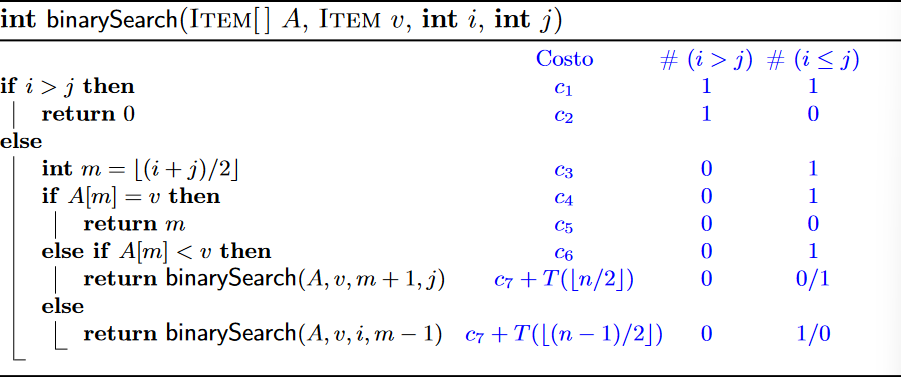
\includegraphics[width=0.9\textwidth]{01/calcoloBinarySearch.png}
            
            A questo punto dobbiamo fare delle assunzioni:
            \begin{itemize}
                \item Assumiamo che la $ n $ potenza di $ 2 $ sia: $ n = 2^k $.
                \item L'elemento cercato non è presente.
                \item Ad ogni passo andiamo sempre a destra in quanto il numero di elementi da valutare è maggiore: $ n/2 $.
            \end{itemize}
            possiamo ora suddividere il problema in due casistiche:
            $$
                \begin{aligned}
                    i>j\quad & (n=0) & T(n)=&c_1 + c_2\\
                    i\leq j\quad & (n>0) & T(n)=&T(n/2) + c_1 + c_2 + c_3 + c_4 + c_6 + c_7\\
                        &&=&T(n/2) + d
                \end{aligned}
            $$
            unendo i due casi otteniamo la \textbf{Relazione di ricorrenza}:
            $$
                T(n)=
                    \begin{cases}
                        c& \text{se } n=0\\
                        T(n/2) +d & \text{se } n>0
                    \end{cases}
            $$
            ottenuta la relazione generalmente per un numero $ n $ di elementi otteniamo che il tempo è dato da:
            $$
                \begin{aligned}
                    T(n)=&T(n/2)+d&\\
                    =&T(n/4)+2d&\\
                    &\hdots\\
                    =&T(1)+kd&\\
                    =&T(0)+(k+1)d&\\
                    =&kd+(c+d) &= d\log n + e
                \end{aligned}
            $$
            ottenendo quindi che il tempo di calcolo è $ O(\log n) $ di natura logaritmica.
    \subsection{Ordini di Complessità}
        \begin{table}[h]
            \centering
            \begin{tabular}{|c|c|c|c|c|c|}
                \hline
                $ f(n) $ & $ n=10^1 $ & $ n=10^2 $ & $n=10^3 $ & $n=10^4 $ & \textbf{Tipo} \\
                \hline
                $ \log n $ & 3 & 6 & 9 & 13 & Logaritmica \\
                \hline
                $ \sqrt{n} $ & 3 & 10 & 31 & 100 & sub-lineare \\
                \hline
                $ n $ & 10 & 100 & 1000 & 10000 & Lineare \\
                \hline
                $ n\log n $ & 30 & 664 & 9965 & 132877 & log-lineare \\
                \hline
                $ n^2 $ & $10^2$ & $10^4$ & $10^6$ & $10^8$ & Quadratica \\
                \hline
                $ n^3 $ & $10^3$ & $10^6$ & $10^9$ & $10^{12}$ & Cubica \\
                \hline
                $ 2^n $ & $1024$ & $10^{30}$ & $10^{301}$ & $10^{3010}$ & Esponenziale\\
                \hline
            \end{tabular}
        \end{table}
\section{Notazione asintotica}
\label{sec:notazioneAsintotica}
    \subsection{Notazioni \texorpdfstring{$ O $, $ \Omega $, $ \Theta $}{O, Omega, Theta}}
        \subsubsection{Notazione $ O $}
            \begin{definition}
                Sia $ g(n) $ una funzione di costo; indichiamo con $ O(g(n)) $ l'insieme delle funzioni $ f(n) $ tali per cui: 
                $$ \exists c>0,\ \exists m\geq 0: f(n) \leq cg(n),\ \forall n\geq m $$
            \end{definition}
            La seguente notazione si legge: $ f(n) $ è "O grande" (big O) di $ g(n) $, con un abuso di notazione si scrive $ f(n)=O(g(n)) $\footnote{\label{fn:note1} Questo è un abuso di notazione in quanto $ O(g(n)) $ è una classe di funzioni e non può essere eguagliata una singola funzione, il simbolo più appropriato sarebbe $ f(n)\in O(g(n)) $}
            . Inoltre per la precedente definizione possiamo dire che $ g(n) $ è un \textbf{limite asintotico superiore} per $ f(n) $, in quanto dopo qualche valore $ m $ la funzione $ g(n) $ è sempre maggiore di $ f(n) $. Inoltre per questo motivo sappiamo che $ f(n) $ cresce al più come $ g(n) $.
        \subsubsection{Notazione $ \Omega $}
            \begin{definition}
                Sia $ g(n) $ una funzione di costo; indichiamo con $ \Omega(g(n)) $ l'insieme delle funzioni $ f(n) $ tali per cui: 
                $$ \exists c>0,\ \exists m\geq 0: f(n) \geq cg(n),\ \forall n\geq m $$
            \end{definition}
            La seguente notazione si legge: $ f(n) $ è "Omega" di $ g(n) $, con un abuso di notazione si scrive $ f(n)=\Omega(g(n)) $\footref{fn:note1}. Inoltre per la precedente definizione possiamo dire che $ g(n) $ è un \textbf{limite asintotico inferiore} per $ f(n) $, in quanto dopo qualche valore $ m $ la funzione $ g(n) $ è sempre minore di $ f(n) $. Inoltre per questo motivo sappiamo che $ f(n) $ cresce almeno come $ g(n) $.
        \subsubsection{Notazione $ \Theta $}
            \begin{definition}
                Sia $ g(n) $ una funzione di costo; indichiamo con $ \Theta(g(n)) $ l'insieme delle funzioni $ f(n) $ tali per cui: 
                $$ \exists c_1>0,\ \exists c_2>0,\ \exists m\geq 0: c_1g(n) \leq f(n) \leq c_2g(n),\ \forall n\geq m $$
            \end{definition}
            La seguente notazione si legge: $ f(n) $ è "Theta" di $ g(n) $, con un abuso di notazione si scrive $ f(n)=\Theta(g(n)) $\footref{fn:note1}. Inoltre per la precedente definizione possiamo dire che $ f(n) $ cresce esattamente come $ g(n) $, detto ciò $ f(n)= \Theta(g(n)) $ se e solo se $ f(n)=O(g(n)) $ e $ f(n)=\Omega(g(n)) $.
        \subsubsection*{Esempio grafico}
            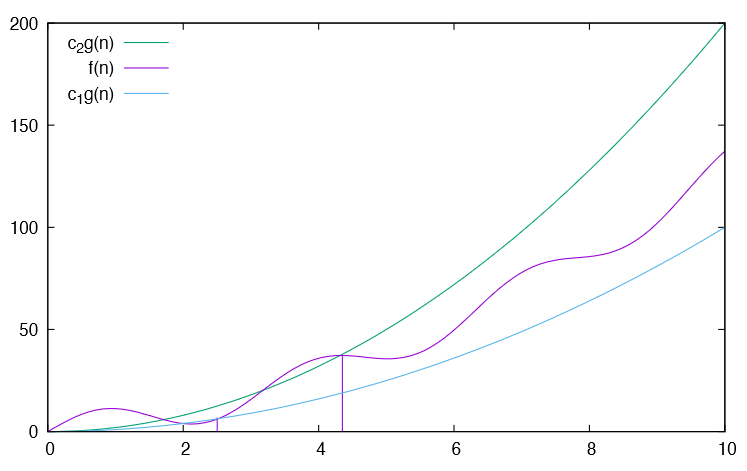
\includegraphics[width=0.5\textwidth]{01/graficoNotazioni.png}
    \subsection{Esempi e Esercizi}
        \subsubsection{Esempio 1}
            $$
                f(n) = 10n^3 + 2n^2 + 7 \stackrel{?}{=} O(n^3)
            $$
            Dobbiamo provare che $ \exists c>0,\ \exists m\geq 0: f(n) \leq cn^3,\ \forall n\geq m $.
            $$
                \begin{aligned}
                    f(n) =& 10n^3 + 2n^2 + 7\\
                    \leq & 10n^3 + 2n^3 + 7 &\quad \forall n \geq 1\\ 
                    \leq & 10n^3 + 2n^3 + n^3 &\quad  \forall n \geq \sqrt[3]{7}\\
                    = & 13 n^3 \stackrel{?}{\leq} cn^3
                \end{aligned}
            $$
            Che è verificata per qualsiasi $ c \geq 13 $ e $ m \geq \sqrt[3]{7} $, arrotondiamo $m$ ad un intero superiore ottenendo $ m = 2 $. 
            
            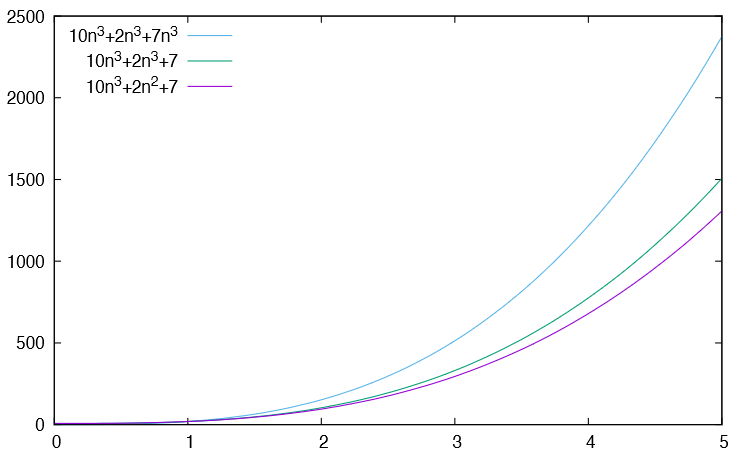
\includegraphics[width=0.5\textwidth]{01/graficoEs1.png}
\section{Complessità problemi v/s algoritmi}
    \subsection{Moltiplicazione numeri complessi}
        Per moltiplicare numeri complessi bisogna svolgere la seguente operazione:
        $$
            (a+bi)(c+di) = [ac-bd]+[ad+bc]i
        $$
        dunque dai parametri $ a,b,c,d $ otteniamo che il risultato da restituire: $ ac-bd $ e $ ad+bc $.
        \paragraph{Domande}
            Considerando che addizioni e sottrazioni costino $ c_1 = 0.01 $ e moltiplicazione costi $ c_2 = 1 $ possiamo chiederci:
            \begin{itemize}
                \item Quanto costa l'algoritmo?
                \item Si può fare meglio?
                \item Qual'è il ruolo del modello di calcolo?
            \end{itemize}
            Dato che si devono fare almeno 4 moltiplicazioni e 2 somme otteniamo che il costo totale è $ 4c_2 + 2c_1 = 4.02 $.
            
            Ora si può fare meglio? La risposta è no in quanto se si potesse fare meglio si potrebbe fare meglio allora bisognerebbe trovare un algoritmo che esegua meno di 4 moltiplicazioni e 2 somme, ma per fare ciò bisognerebbe cambiare il modello di calcolo.
    \subsection{Sommare numeri binari}
        \subsubsection{Algoritmo elementare della somma - $ \operatorname{sum}() $}
            Ipotizziamo che l'operazione da fare sia la somma di due bit singoli e generare il riporto, assegniamo a questa operazione costo $ c $.
            Dopo ciò indichiamo con $ n $ il numero massimo di bit tra i due numeri da sommare, otteniamo dunque che:
            \begin{itemize}
                \item Richiede di esaminare tutti gli $ n $ bit
                \item Costo totale $ cn = O(n) $
            \end{itemize}
        \subsubsection{Esiste allora un algoritmo più efficiente?}
            La risposta è no in quanto se esistesse un algoritmo di tale genere allora potremmo cambiare un solo bit di uno dei due numeri e ottenere un risultato diverso senza che l'algoritmo lo vada ad analizzare, il che è impossibile.
    \subsection{Moltiplicare numeri binari}
        \subsubsection{Algoritmo elementare del prodotto - $\operatorname{prod}()$}
            L'operazione elementare per moltiplicare due numeri binari è la seguente:
            $$
                \begin{array}{c c c c c c c c c c c c c c c}
                    & & & & & & & 1 & 0 & 1 & 1 & 1 & 0 & 1 & *\\
                    & & & & & & & 1 & 1 & 0 & 1 & 1 & 1 & 0 & \\
                    \hline
                    & & & & & & & 0 & 0 & 0 & 0 & 0 & 0 & 0 &\\
                    & & & & & & 1 & 0 & 1 & 1 & 1 & 0 & 1 & &\\
                    & & & & & 1 & 0 & 1 & 1 & 1 & 0 & 1 & & &\\
                    & & & & 1 & 0 & 1 & 1 & 1 & 0 & 1 & & & &\\
                    & & & 0 & 0 & 0 & 0 & 0 & 0 & 0 & & & & &\\
                    & & 1 & 0 & 1 & 1 & 1 & 0 & 1 & & & & & &\\
                    & 1 & 0 & 1 & 1 & 1 & 0 & 1 & & & & & & &\\
                    \hline
                    1 & 0 & 0 & 1 & 1 & 1 & 1 & 1 & 1 & 1 & 0 & 1 & 1 & 0\\
                \end{array}
            $$
            deduciamo che:
            \begin{itemize}
                \item Dobbiamo accedere a tutti i bit
                \item Il costo totale è $ cn^2 = O(n^2) $ perché dobbiamo fare $ n $ somme di $ n $ bit.
            \end{itemize}
        \subsubsection{Soluzione Divide-et-impera}
            La base del principio \textbf{Divide-et-impera} è la seguente:
            \begin{description}
                \item[Divide] Dividere il problema in sotto-problemi più piccoli.
                \item[Impera] risolvi i sotto-problemi in modo ricorsivo.
                \item[Combina] combina le soluzioni dei sotto-problemi per ottenere la soluzione del problema originale.  
            \end{description}
            La soluzione divide-et-impera per il problema della moltiplicazione binaria è la seguente:
            $$
                \begin{aligned}
                    \begin{aligned}
                        X=& a\cdot 2^{n/2} + b\\
                        Y=& c\cdot 2^{n/2} + d\\
                        XY =& ac\cdot 2^n + (ad+bc)\cdot 2^{n/2} + bd
                    \end{aligned}
                    &\quad
                    \begin{aligned}
                        X &= \stackrel{a}{\text{Parte SX}}\quad \stackrel{b}{\text{Parte DX}}\\
                        Y &= \stackrel{c}{\text{Parte SX}}\quad \stackrel{d}{\text{Parte DX}}
                    \end{aligned}
                \end{aligned}
            $$
            Ora possiamo scrivere l'algoritmo:
            \begin{algorithm}
                \caption{boolean[ ] pdi(boolean[ ] X, boolean[ ] Y, int n)}\label{alg:pdi}
                \begin{algorithmic}[1]
                    \If{$n=1$}
                        \State \Return $X[1]\cdot Y[1]$
                    \Else
                        \State spezza $X$ in $a$ e $b$ e $Y$ in $c$ e $d$
                        \State \Return pdi($a,c,n/2$)$\cdot 2^n$ + (pdi($a,d,n/2$) + pdi($b,c,n/2$))$\cdot 2^{n/2}$ + pdi($b,d,n/2$)
                    \EndIf
                \end{algorithmic}
            \end{algorithm}
            La funzione di costo associata all'algoritmo è:
            $$
                T(n)=\begin{cases}
                    c_1 & n=1\\
                    4T(n/2)+c_2\cdot n &  n>1
                \end{cases}
            $$
            \textbf{Nota:} moltiplicare per $2^n$ corrisponde a uno shift a sinistra di $n$ posizioni, svolta in tempo lineare.

            Ora in quanto abbiamo $ 4 $ chiamate ricorsive, assumendo che $c_1$ sia il tempo per moltiplicare due bit e che $ c_2 $ sia il tempo per sommare due numeri binari otteniamo che il tempo di calcolo è $ c_2 \cdot 4^i \cdot \frac{n}{2^i} = T(1) \cdot 4^{\log_2 n} = c_1 \cdot n^{\log_2 4} = c_1 \cdot n^2 $.
            \subparagraph{Ma allora è possibile fare meglio?}
            Long story short: si in quanto è stato provato nel 2021 l'esistenza di un algoritmo di complessità $ O(n\log n) $. 
\section{Algoritmi di Ordinamento}
    \paragraph{Introduzione} L'obbiettivo di questa sezione è valutare la complessità degli algoritmi in base all'input, in alcuni casi gli algoritmi si comportano differentemente in base all'input se siamo a conoscenza dell'input questa ci consente di scegliere un algoritmo più adeguato alla nostra soluzione.
    \paragraph{Come analiziamo gli algoritmi}
        Possiamo analizzare l'efficienza degli algoritmi in base a diversi casi:
        \subparagraph{Caso Pessimo}
            Questa analisi è la più importante in quanto sappiamo che questa restituisce il limite superiore al tempo di esecuzione qualsiasi sia l'input.
        \subparagraph{Caso Medio}
            Questa analisi è la più complessa in quanto bisogna definire il "caso medio" e cosa si intende per "medio", ma è utile con una distribuzione uniforme degli input.
        \subparagraph{Caso Ottimo}
            Utile solo se conosciamo qualcosa sull'input, altrimenti non risulta utile se abbiamo un input arbitrario.
    \subsection{Selection Sort}
        Algoritmo Selection Sort:
        \begin{algorithm}
            \caption{selectionSort(Item[ ] A, \Int n)}\label{alg:selectionSort}
            \begin{algorithmic}[1]
                \For{$i=1$ \To $n-1$}
                    \State \Int $min \gets \operatorname{min}(A,i,n)$
                    \State $A[i]$ $\leftrightarrow$ $\operatorname{min}(A,i,n) $
                \EndFor
            \end{algorithmic}
        \end{algorithm}

        Algoritmo di supporto min:
        \begin{algorithm}
            \caption{int min(Item[ ] A, \Int i, \Int n)}\label{alg:min}
            \begin{algorithmic}[1]
                \State \Int min $\gets i$
                \For{$j=i+1$ \To $n$}
                    \If{$A[j]<A[min]$}
                        \State min $\gets j$
                    \EndIf
                \EndFor
                \State \Return min
            \end{algorithmic}
        \end{algorithm}
        Avendo analizzato il seguente algoritmo notiamo come in ogni caso, ottimo, medio e pessimo, il "ciclo" esterno della funzione $ \operatorname{selectionSort}() $ viene eseguito $ n-1 $ volte, mentre il ciclo interno della funzione $ \operatorname{min}() $ viene eseguito $ n-i $ dove $ i $ è il valore dell'iterazione del ciclo esterno, quindi $ n-1 + n-2 + n-3 + \ldots + 1 = \frac{n(n-1)}{2} $ volte, otteniamo quindi che il tempo di calcolo è $ O(n^2) $ in quanto questo si può approssimare a $ \frac{n^2}{2} $.
        $$  
            \sum_{i=1}^{n-1} n-i = \sum_{i=1}^{n-1} i = \frac{n(n-1)}{2}= O(n^2)
        $$
    \subsection{Insertion Sort}
        L'algoritmo di insertion sort è efficiente per ordinare piccoli insiemi, il concetto dietro a questo si bassa sull'inserimento dell'elemento preso in analisi al posto giusto.
        
        Algoritmo Insertion Sort:
        \begin{algorithm}
            \caption{insertionSort(Item[ ] A, \Int n)}\label{alg:insertionSort}
            \begin{algorithmic}[1]
                \For{$i=2$ \To $n$}
                    \State Item $temp \gets A[i]$
                    \State \Int $j \gets i$
                    \While{$j>1$ and $A[j-1]>temp$}
                        \State $A[j] \gets A[j-1]$
                        \State $j \gets j-1$
                    \EndWhile
                    \State $A[j] \gets temp$
                \EndFor
            \end{algorithmic}
        \end{algorithm}
        
        Il costo di esecuzione non dipende esclusivamente dalla dimensione ma anche dall'ordine degli elementi in ingresso.
        \subparagraph{Caso Pessimo} Il costo dunque nel \textbf{caso pessimo} è $ O(n^2) $ in quanto vengono eseguiti $ n-1 $ cicli esterni e $ n-1 $ cicli interni, ottenendo dunque $ (n-1) + (n-2) + \ldots + 1 = \frac{n(n-1)}{2} = O(n^2) $.
        \subparagraph{Caso Medio }Nel \textbf{caso medio} il costo rimane $ O(n^2) $ in quanto il ciclo interni viene eseguito $ n/2 $ volte, ottenendo dunque $ \frac{n(n-1)}{4} = O(n^2) $.
        \subparagraph{Caso Ottimo} Nel \textbf{caso ottimo} il costo è $ O(n) $ in quanto il ciclo interno non viene mai eseguito.
        
        Questo ci porta a dire che il $ \operatorname{insertionSort}() $ è un algoritmo di ordinamento utile nei casi in cui l'input è già ordinato o quasi ordinato, nei casi nei quali non conosciamo la natura dell'input è meglio utilizzare un algoritmo di ordinamento differente.
    \subsection{Merge Sort}
        L'algoritmo di $ \operatorname{mergeSort}() $ è un algoritmo di ordinamento basato sul principio \textbf{divide-et-impera}.
        \begin{description}
            \item[Divide:] Spezza virtualmente il vettore di $ n $ elementi in sotto-vettori di $ n/2 $ elementi.
            \item[Impera:] Chiama $ \operatorname{mergeSort}() $ ricorsivamente sui due sotto-vettori.
            \item[Combina:] Unisci (\textbf{merge}) i due sotto-vettori ordinati in un unico vettore ordinato. 
        \end{description}
        In input si ha:
        \begin{itemize}
            \item $ A $: vettore di $ n $ elementi.
            \item $ \text{start}, \text{end}, \text{mid} $ sono tali che $ 1\leq \text{start} < \text{mid} < \text{end} \leq n $.
            \item I sotto-vettori $ A[\text{start},\ldots,\text{mid}] $ e $ A[\text{mid}+1,\ldots,\text{end}] $ sono ordinati.
        \end{itemize}
        In output si hanno i due sotto-vettori fusi in un unico sotto-vettore ordinato, tramite un vettore di appoggio $ B $.

        Funzione di appoggio $\operatorname{Merge}$:
        \begin{algorithm}
            \caption{Merge(Item[ ] A, \Int start, \Int end, \Int mid)}\label{alg:merge}
            \begin{algorithmic}[1]
                \State \Int $i,j,k,h$
                \State \Int $i \gets \text{start}$
                \State \Int $j \gets \text{mid}+1$
                \State \Int $k \gets \text{start}$
                \While {$i \leq \text{mid}$ and $j \leq \text{end}$}
                    \If{$A[i] \leq A[j]$}
                        \State $B[k] \gets A[i]$
                        \State $i \gets i+1$
                    \Else
                        \State $B[k] \gets A[j]$
                        \State $j \gets j+1$
                    \EndIf
                    \State $k \gets k+1$
                \EndWhile
                \State $j \gets \text{end}$
                \For {$h=\text{mid}$ \DownTo $i$}
                    \State $A[j] \gets A[h]$
                    \State $j \gets j-1$
                \EndFor
                \For {$j=\text{start}$ \To $k-1$}
                    \State $A[j] \gets B[j]$
                \EndFor
            \end{algorithmic}
        \end{algorithm}
        
        Il costo computazionale di $ \operatorname{Merge}() $ è $ O(n) $, questa è la base del costo computazionale di $ \operatorname{mergeSort}() $.
        \newpage % Usato per evitare che l'algoritmo venga spezzato tra due pagine diverse
        Funzione completa $ \operatorname{mergeSort}() $:

        \begin{algorithm}
            \caption{mergeSort(Item[ ] A, \Int start, \Int end)}\label{alg:mergeSort}
            \begin{algorithmic}[1]
                \If{$\text{start}<\text{end}$}
                    \State \Int $mid \gets (\text{start}+\text{end})/2$
                    \State mergeSort($A,\text{start},\text{mid}$)
                    \State mergeSort($A,\text{mid}+1,\text{end}$)
                    \State merge($A,\text{start},\text{end},\text{mid}$)
                \EndIf
            \end{algorithmic}
        \end{algorithm}

        Assumendo per semplificare che $ n = 2^k $ dove $ k $ è un intero allora l'altezza dell'albero è esattamente $ k = \log n $, in questo modo tutti i sotto-vettori hanno dimensione che è potenza di 2.
        Così facendo il costo computazionale di $ \operatorname{mergeSort}() $ è:
        $$
            T(n)=\begin{cases}
                c & n=1\\
                2T(n/2)+dn & n>1
            \end{cases}
        $$
        dove $ c $ è il costo di un'operazione elementare, $ d $ è il costo di $ \operatorname{Merge}() $ e $ n $ è il costo di copiare i valori da $ B $ a $ A $.
    \chapter{Analisi di funzioni}
\thispagestyle{chapterInit}
\section{Notazione asintotica}
    \subsection{Definizioni}
        Si rimanda al \hyperref[sec:notazioneAsintotica]{sezione 1.2} per le definizioni di $O$, $\Omega$ e $\Theta$.
\section{Proprietà della notazione asintotica}
    \subsection{Regola Generale}
        Da qui si prende in considerazione la seguente espressione polinomiale:
        $$
            f(n) = a_kn^k + a_{k-1}n^{k-1} + \ldots + a_1n + a_0, \quad a_k > 0 \Rightarrow f(n) = \Theta(n^k)
        $$
        \paragraph{Limite Superiore} $ \exists c>0, \exists m\geq 0: f(n)\leq cn^k,\forall n\geq m $
            $$
                \begin{aligned}
                    f(n)=&a_kn^k + a_{k-1}n^{k-1} + \ldots + a_1n + a_0 \\
                    \leq& a_kn^k + \left|a_{k-1}\right|n^{k-1} + \ldots + \left|a_1\right|n + \left|a_0\right| \\
                    \leq& a_kn^k + \left|a_{k-1}\right|n^k + \ldots + \left|a_1\right|n^k + \left|a_0\right|n^k \\
                    =& (a_k + \left|a_{k-1}\right| + \ldots + \left|a_1\right| + \left|a_0\right|)n^k \quad& \forall n\geq 1\\
                    \stackrel{?}{\leq}& cn^k
                \end{aligned}
            $$
            questa è vera per $ c\geq \left(a_k + \left|a_{k-1}\right| + \ldots + \left|a_1\right| + \left|a_0\right| \right) >0$ e per $m=1$
        \paragraph{Limite Inferiore} $ \exists d > 0, \exists m\geq 0: f(n)\geq dn^k,\forall n\geq m $
            $$
                \begin{aligned}
                    f(n)=&a_kn^k + a_{k-1}n^{k-1} + \ldots + a_1n + a_0 \\
                    \geq& a_kn^k - \left|a_{k-1}\right|n^{k-1} - \ldots - \left|a_1\right|n - \left|a_0\right| \\
                    \geq& a_kn^k - \left|a_{k-1}\right|n^k - \ldots - \left|a_1\right|n^k - \left|a_0\right|n^k \\
                    =& (a_k - \left|a_{k-1}\right| - \ldots - \left|a_1\right| - \left|a_0\right|)n^k \quad& \forall n\geq 1\\
                    \stackrel{?}{\geq}& dn^k
                \end{aligned}
            $$
            questa è vera se: $ d\leq a_k - \frac{\left|a_{k-1}\right|}{n} - \ldots - \frac{\left|a_1\right|}{n} - \frac{\left|a_0\right|}{n} >0 \Leftrightarrow n>\frac{\left|a_{k-1}\right| + \ldots + \left|a_1\right| + \left|a_0\right|}{a_k} $     
        \subsubsection{Casi Particolari}
            \paragraph{Complessità di $ f(n) = 5 $}
                $$
                    \begin{aligned}
                        f(n) = 5 \geq c_1n^0 \Rightarrow c_1\leq 5 \\
                        f(n) = 5 \leq c_2n^0 \Rightarrow c_2\geq 5 \\
                        \Rightarrow f(n) = \Theta(n^0) = \Theta(1)
                    \end{aligned}
                $$
            \paragraph{Complessità di $ f(n) = 5 + \sin(n) $}
                La complessità di calcolo di $ f(n) $ è $ \Theta(1) $, in quanto $ \sin(n) $ è una funzione oscillante tra $ -1 $ e $ 1 $, quindi $ 5 + \sin(n) $ oscilla tra $ 4 $ e $ 6 $.

                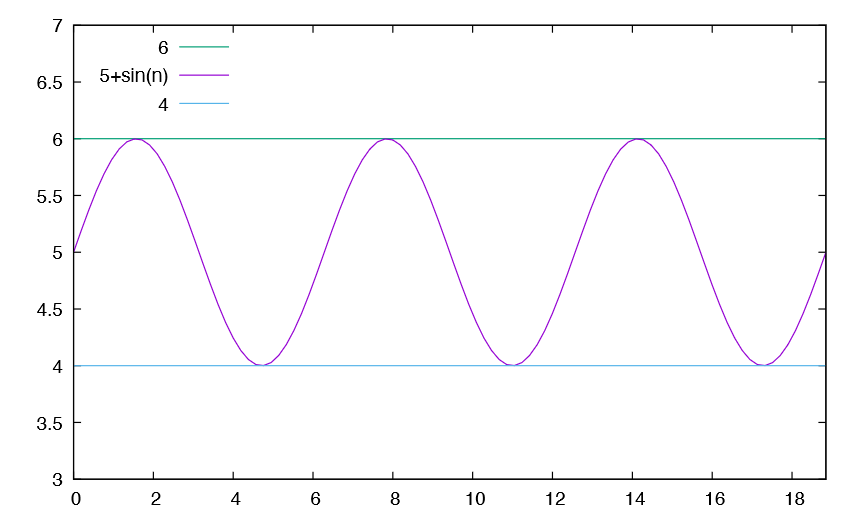
\includegraphics[scale=0.5]{02/graficoFsin.png}
    \subsection{Proprietà delle notazioni}
        \subsubsection{Dualità}
            $ f(n) = O(g(n)) \Leftrightarrow g(n) = \Omega(f(n)) $
            \begin{proof}
                $$
                    \begin{aligned}
                        f(n) = O(g(n)) \Leftrightarrow & f(n) \leq cg(n), \forall n\geq m \\
                        \Leftrightarrow & g(n) \geq \frac1cf(n), \forall n\geq m \\
                        \Leftrightarrow & g(n) \geq c'f(n), \forall n\geq m, c'=\frac1c \\
                        \Leftrightarrow & g(n) = \Omega(f(n))
                    \end{aligned}
                $$
            \end{proof}
        \subsubsection{Eliminazione di costanti}
            $$
                \begin{aligned}
                    f(n) &= O(g(n)) \Leftrightarrow af(n)=O(g(n)), \forall a>0 \\
                    f(n) &= \Omega(g(n)) \Leftrightarrow af(n)=\Omega(g(n)), \forall a>0 \\
                \end{aligned}
            $$
            \begin{proof}                
                $$
                    \begin{aligned}
                        f(n)=O(g(n)) \Leftrightarrow & f(n)\leq cg(n), \forall n\geq m \\
                        \Leftrightarrow & af(n)\leq acg(n), \forall n\geq m,\forall a>0 \\
                        \Leftrightarrow & af(n)\leq c'g(n), \forall n\geq m,c'=ac>0 \\
                        \Leftrightarrow & af(n)=O(g(n)), \forall a>0
                    \end{aligned}
                $$
            \end{proof}
        \subsubsection{Sommatoria (sequenza di algoritmi)}
            $$
                \begin{aligned}
                    f_1(n) = O(g_1(n)), f_2(n) = O(g_2(n)) \Rightarrow f_1(n) + f_2(n) = O(\max(g_1(n),g_2(n)))\\
                    f_1(n) = \Omega(g_1(n)), f_2(n) = \Omega(g_2(n)) \Rightarrow f_1(n) + f_2(n) = \Omega(\max(g_1(n),g_2(n)))
                \end{aligned}
            $$
            \begin{proof}[Dimostrazione (Lato $ O $).]
                $$
                    \begin{aligned}
                        f_1(n) = O(g_1(n)) \land f_2(n) = O(g_2(n)) & \Rightarrow \\
                        f_1(n) \leq c_1g_1(n) \land f_2(n) \leq c_2g_2(n) & \Rightarrow \\
                        f_1(n) + f_2(n) \leq c_1g_1(n) + c_2g_2(n) & \Rightarrow \\
                        f_1(n) + f_2(n) \leq \max\{c_1,c_2\}(2\cdot \max(g_1(n),g_2(n))) & \Rightarrow \\
                        f_1(n) + f_2(n) = O(\max(g_1(n),g_2(n))) &
                    \end{aligned}
                $$
            \end{proof}
        \subsubsection{Prodotto (cicli annidati)}
            $$
                \begin{aligned}
                    f_1(n) = O(g_1(n)), f_2(n) = O(g_2(n)) \Rightarrow f_1(n) \cdot f_2(n) = O(g_1(n) \cdot g_2(n))\\
                    f_1(n) = \Omega(g_1(n)), f_2(n) = \Omega(g_2(n)) \Rightarrow f_1(n) \cdot f_2(n) = \Omega(g_1(n) \cdot g_2(n))
                \end{aligned}
            $$
            \begin{proof}
                $$
                    \begin{aligned}
                        f_1(n) = O(g_1(n)) \land f_2(n) = O(g_2(n)) & \Rightarrow \\
                        f_1(n) \leq c_1g_1(n) \land f_2(n) \leq c_2g_2(n) & \Rightarrow \\
                        f_1(n)\cdot f_2(n) \leq c_1c_2g_1(n)g_2(n) &
                    \end{aligned}
                $$
        \end{proof}
        \subsubsection{Simmetria}
            $$
                f(n) = \Theta(g(n)) \Leftrightarrow g(n) = \Theta(f(n))
            $$
            \begin{proof}
                Grazie alla proprietà della dualità, si ha che:
                $$
                    \begin{aligned}
                        f(n) = \Theta(g(n)) &\quad \Rightarrow \quad f(n) = O(g(n)) \Rightarrow g(n) = \Omega(f(n))\\
                        f(n) = \Theta(g(n)) &\quad \Rightarrow \quad f(n) = \Omega(g(n)) \Rightarrow g(n) = O(f(n))
                    \end{aligned}
                $$
            \end{proof}
        \subsubsection{Transitività}
            $$
                \begin{aligned}
                    f(n) = O(g(n)), g(n) = O(h(n)) \Rightarrow f(n) = O(h(n))
                \end{aligned}
            $$
            \begin{proof}
                $$
                    \begin{aligned}
                        f(n) = O(g(n)) \land g(n) = O(h(n)) & \Rightarrow \\
                        f(n) \leq c_1g(n) \land g(n) \leq c_2h(n) & \Rightarrow \\
                        f(n) \leq c_1c_2h(n) & \Rightarrow \\
                        f(n) = O(h(n)) &
                    \end{aligned}
                $$
            \end{proof}
    \subsection{Altre funzioni di costo}
        \subsubsection{Logaritmi v/s funzioni lineari}
            \paragraph{Proprietà dei Logaritmi}
                Vogliamo provare che $ \log(n) = O(n) $. Dimostriamo per induzione che
                $$
                    \exists c>0,\exists m\geq 0:\log n\leq cn,\forall n\geq m\qquad \text{definizione di }O
                $$
                \begin{proof}
                    \begin{basecase} ($ n=1 $):
                        $ \log 1 = 0 \leq \stackrel{c}0\cdot \stackrel{n}1 = 0 $
                    \end{basecase}
                    \textbf{Ipotesi induttiva}: sia $ \log k \leq ck, \forall k\leq n $.
                    \begin{inductivecase}
                        Dimostriamo la proprietà per $ n+1 $:
                        $$
                            \begin{aligned}
                                \log(n+1) \leq & \log(n+n) = \log 2n & \forall n\geq 1 \\
                                = & \log 2 + \log n \qquad & \log ab = \log a + \log b \\
                                = & 1 + \log n & \log 2 = 1 \\
                                \leq & 1 + cn & \text{per induzione} \\
                                \stackrel{?}{\leq} & c(n+1) & \text{Obbiettivo} \\
                                1+cn\leq c(n+1) \Leftrightarrow & c\geq 1
                            \end{aligned}
                        $$
                    \end{inductivecase}
                \end{proof}
        \subsection{Giocando con le espressioni}
            \paragraph{Es 1}
                È vero che $ \log_a n = \Theta(\log n) $?

                Si: $ \log_a n = (\log_a 2) \cdot (\log_2 n) = \Theta(\log n) $
            
            \paragraph{Es 2}
                È vero che $ \log n^a = \Theta(\log n) $, per $ a>0 $?

                Si: $ \log n^a = a\log n = \Theta(\log n) $
            
            \paragraph{Es 3}
                È vero che $ 2^{n+1} = \Theta(2^n) $?

                Si: $ 2^{n+1} = 2\cdot 2^n = \Theta(2^n) $
            \paragraph{Es 4}    
                È vero che $ 2^{n} = \Theta(3^n) $?

                Ovviamente $ 2^{n} = O(3^n) $

                Ma: $ 3^{n} = \left(\frac32\cdot 2\right)^n=\left(\frac32\right)^n\cdot 2^n: $ Quindi non esiste $ c > 0 $ tale per cui $ \left(\frac32\right)^n\cdot 2^n\leq c2^n $, quindi $ 2^n \neq O(3^n) $
    \subsection{Classificazione delle funzioni}
        È possibile definire un ordinamento delle principali classi estendendo le relazioni che abbiamo dimostrato:
        
        Per ogni $r<s,h<k,a<b$:
        $$
            o(1) \subset O(\log^r n) \subset O(\log^s n) \subset O(n^h) \subset O(n^h \log^r n ) \subset O(n^h \log^s n) \subset O(n^k) \subset O(a^n) \subset O(b^n)
        $$
\section{Ricorrenze}
    \subsection{Introduzione}
        \paragraph{Equazioni di ricorrenza} Quando si calcola la complessità di un algoritmo ricorsivo, questa viene espressa tramite un'\textbf{equazione di ricorrenza}, ovvero una formula definita in maniera ricorsiva.
            \subparagraph{MergeSort}
                $$
                    T(n) = \begin{cases}
                        1 & \text{se } n=1 \\
                        2T\left(\frac{n}{2}\right) + n & \text{se } n>1
                    \end{cases}
                $$
        \paragraph{Forma Chiusa} L'obbiettivo è quello di ottenere, quando possibile, una \textbf{formula chiusa} che rappresenti la classe di complessità della funzione.
            \subparagraph{MergeSort}
                $$ 
                    T(n) = \begin{cases}
                        T(\lfloor n/2 \rfloor) + T(\lceil n/2 \rceil) + \Theta(n) & n > 1 \\
                        \Theta(1) & n \leq 1
                    \end{cases} \Longrightarrow T(n) = \Theta(n\log n)
                $$
    \subsection{Metodo dell'albero di ricorsione, o per livelli}
        \paragraph{Introduzione} "Srotoliamo" la ricorrenza in un albero i costi ai vari livelli della ricorsione.
        \subsubsection{Esempio 1}
            $$
                T(n)=\begin{cases}
                    T(n/2) + b & n>1 \\
                    c & n\leq 1
                \end{cases}
            $$
            È possibile risolvere questa ricorrenza nel modo seguente:
            $$
                \begin{aligned}
                    T(n) = & b + T(n/2) \\
                    = & b + b + T(n/4) \\
                    = & b + b + b + T(n/8) \\
                    = & \ldots \\
                    = & \underbrace{b+b+\ldots+b}_{\log n} + T(1) \\
                \end{aligned}
            $$
            Assumiamo per semplicità che $ n=2^k $. $ T(n) = b\log n + c = \Theta(\log n) $
        \subsubsection{Esempio 2}
            $$
                T(n)=\begin{cases}
                    4T(n/2) + n & n>1 \\
                    1 & n\leq 1
                \end{cases}
            $$
            È possibile risolvere questa ricorrenza nel modo seguente:
            $$
                \begin{aligned}
                    T(n)=&\cancel{n\sum_{j=0}^{\log(n-1)} 2^j} &\underbrace{+4^{\log n}}_{\text{somma degli }T(1)}\\
                    \Rightarrow &\underbrace{n\cdot \frac{\overbrace{2^{\log n }}^{n\text{ per prop. log.}}-1}{2-1}}_{\stackrel{\text{usando: }}{\forall x\neq 1:\sum_{j=0}^kx^j=\frac{x^{k+1}-1}{x-1}}}&+4^{\log n}\\
                    =& n(n-1)&+4^{\log n}\\
                    =& n^2-n&\overbrace{+n^2}^{\text{cambiamento di base}}\\
                    =& 2n^2-n = \Theta(n^2)
                \end{aligned}
            $$
        \subsubsection{Esempio 3}
        $$
            T(n)=\begin{cases} 4T(n/2) + n^3 & n>1 \\ 1 & n\leq 1 \end{cases}
        $$
        Da questa equazione notiamo che il primo livello ha costo $ n^3 $, il secondo $ 4\left(\frac{n}{2}\right)^3 $ il terzo $ 4^2\left(\frac{n}{2^2}\right)^3 $ e così via. Quindi possiamo scrivere la sommatoria:
        $$
            \begin{aligned}
                T(n)=& n^3 + 4\left(\frac{n}{2}\right)^3 + \ldots + 4^{\log n-1}\left(\frac{n}{2^{\log n-1}}\right)^3 &+ 4^{\log n} \\
                =& \sum_{i=0}^{\log n-1}4^i\left(\frac{n}{2^i}\right)^3 & + 4^{\log n} \\
                =& n^3\sum_{i=0}^{\log n-1}\left(\frac{2^{2i}}{2^{3i}}\right) & + 4^{\log n} \\
                =& n^3\sum_{i=0}^{\log n-1}\left(2^{2i-3i}\right) & + 4^{\log n} \\
                =& n^3\sum_{i=0}^{\log n-1}\left(2^{-1\cdot i}\right) & + 4^{\log n} \\
                =& n^3\sum_{i=0}^{\log n-1}\left(\frac{1}{2}\right)^i & \overbrace{+n^2}^{\text{cambiamento di base}} \\
                \leq & n^3\sum_{i=0}^{\infty}\left(\frac{1}{2}\right)^i & +n^2 \\
                =& n^3\cdot \overbrace{\frac{1}{1-\frac{1}{2}}}^{\text{usando: }\forall x,|x|\leq 1:\sum_{i=0}^{\infty}x^i=\frac{1}{1-x}} & +n^2 \\
                =& 2n^3 + n^2
            \end{aligned}
        $$
        \footnote{In quanto la sommatoria tende a crescere allora abbiamo potuto sostituire $ \log n $ con $ \infty $ e modificare il segno di uguaglianza con quello di $ \leq $ in quanto la sommatoria verso l'infinito converge è più grande di quella finita}\newline
        Abbiamo dunque dimostrato che $ T(n) \leq 2n^3 + n^2 = O(n^3) $ però non possiamo, tramite la dimostrazione precedente, dire che $ T(n) = \Theta(n^3) $ in quanto siamo passati ad una disequazione. In questo particolare caso d'altra parte possiamo notare che $ T(n) \geq n^3 $ il che ci porta ad affermare che $ T(n) = \Omega(n^3) $ e quindi $ T(n) = \Theta(n^3) $. 
    \subsection{Metodo di sostituzione}
        \paragraph{Introduzione} È il metodo in cui si cerca di \textbf{indovinare} (\textbf{guess}) la soluzione e si prova a dimostrarla per \textbf{induzione}.
        \subsubsection{Primo esempio}
            $$ T(n) = \begin{cases} T(\lfloor n/2 \rfloor) + n & n>1 \\ 1 & n\leq 1 \end{cases} $$
            Notiamo come il costo dei vali livelli sia $ n + n/2 + n/4 + \ldots $. Dunque possiamo ipotizzare di poter scrivere:
            $$
                \begin{aligned}
                    T(n)=& n \cdot \sum_{i=0}^{\log n}\left(\frac{1}{2}\right)^i\\
                    \leq & n \cdot \sum_{i=0}^{\infty}\left(\frac{1}{2}\right)^i\\
                    = & n \cdot \underbrace{\frac{1}{1-\frac{1}{2}}}_{\text{usando }\forall x,|x| < 1: \sum_{i=0}^{\infty}x^i=\frac{1}{1-x}}\\
                    = & 2n
                \end{aligned}
            $$
            \footnote{Abbiamo potuto usare il $ \leq $ in quanto la sommatoria in questione all'infinito è sempre maggiore di quella finita e ci stiamo calcolando il costo massimo}
            \paragraph{Limite superiore}
                Tentiamo quindi ora di dire che $ T(n) = O(n) $:
                \subparagraph{Caso Base} $ T(1) = 1 \stackrel{?}{\leq} 1 \cdot c \Leftrightarrow \forall c\geq 1 $
                \subparagraph{Passo Induttivo} Dimostriamo la disequazione per $T(n)$
                $$
                    \begin{aligned}
                        T(n) = & T(\lfloor n/2 \rfloor) + n \\
                        \leq & \overbrace{c\lfloor n/2 \rfloor}^{\text{ipotizzato} O(n)} + n \\
                        \leq & c\cdot\overbrace{n/2}^{\text{intero inferiore}} + n \\
                        = & n(c/2 + 1) \\
                        \stackrel{?}{\leq} & cn \\
                        \Leftrightarrow & c/2 + 1 \leq c \Leftrightarrow c\geq 2
                    \end{aligned}
                $$
                
                Dunque abbiamo provato che: $ T(n) \leq cn $, nel caso base $ c\geq 1 $ e nel passo induttivo $ c\geq 2 $. In quanto deve valere per entrambi i casi allora il primo valore utile di $ c $ è $2$, avendo provato che per $ n=1 $ la disequazione vale e che per tutti i successivi valori di $ n $ la disequazione vale allora possiamo dire che $ T(n) = O(n) $.
            \paragraph{Limite Inferiore}
                Tentiamo di dimostrare che $ T(n) = \Omega(n) $:
                \subparagraph{Caso Base} Dimostriamo che $ T(1) = 1 \stackrel{?}{\geq} 1\cdot d \Leftrightarrow \forall d\leq 1 $
                \newpage % Per evitare che il passo induttivo vada a capo
                \subparagraph{Passo Induttivo} Dimostriamo la disequazione per $ T(n) $:
                $$
                    \begin{aligned}
                        T(n) =& T(\lfloor n/2 \rfloor) + n \\
                        \geq & \overbrace{d\lfloor n/2 \rfloor}^{\text{per ipo. induttiva sostituzione}} + n \\
                        \geq & d\cdot\overbrace{\frac{n}2-1}^{\text{intero inferiore}} + n \\
                        = & \left(\frac{d}2-\frac1n+1\right)n \stackrel{?}{\geq} dn \\
                        \Leftrightarrow & \frac{d}2-\frac1n+1 \geq d \\ 
                        \Leftrightarrow & d\leq 2 - \frac2n
                    \end{aligned}
                $$

                Abbiamo quindi dimostrato che $ T(n) \geq dn $, nel caso base $ d\leq 1 $ e nel passo induttivo $ d\leq 2 - \frac2n $. In quanto deve valere per entrambi i casi allora il primo valore utile di $ d $ è $1$, avendo provato che per $ n=1 $ la disequazione vale e che per tutti i successivi valori di $ n $ la disequazione vale allora possiamo dire che $ T(n) = \Omega(n) $.
                
            \paragraph{Conclusione} Avendo provato che $ T(n) = O(n) $ e $ T(n) = \Omega(n) $ e ricordando che se $ T(n) = O(n) \land T(n) = \Omega(n) \Leftrightarrow T(n) = \Theta(n) $ concludendo che la funzione di costo di $ T(n) $ cresce in maniera lineare.
        \subsubsection{Terzo esempio - Difficoltà matematiche}
            $$
                T(n)=\begin{cases} T\left(\left\lfloor\frac{n}2\right\rfloor\right) + T\left(\left\lceil\frac{n}2\right\rceil\right) + 1 & n>1 \\ 1 & n\leq 1 \end{cases}
            $$
            \paragraph{Limite Superiore}
                Dalla seguente si può notare come il costo di ogni livello sia $ 1 $ e che il numero di livelli sia $ \log n $. Inoltre la ricorsione viene eseguita su due rami, quindi possiamo scrivere la seguente sommatoria:
                $$
                    \begin{aligned}
                        T(n)=&\sum_{i=0}^{\log n}2^i\\
                        =&1+2+4+\ldots+\frac{n}4+\frac{n}2+n \\
                        =&O(n)
                    \end{aligned}
                $$
                Proviamo ora a dimostrare che $ T(n) = O(n) $:
                \subparagraph{Passo Induttivo} Ipotizzando che $ \forall k<n:T(k)\leq ck $, dimostriamo che $ T(n)\leq cn $:
                    $$
                        \begin{aligned}
                            T(n)=&T\left(\left\lfloor\frac{n}2\right\rfloor\right) + T\left(\left\lceil\frac{n}2\right\rceil\right) + 1 \\
                            \leq & c\left\lfloor\frac{n}2\right\rfloor + c\left\lceil\frac{n}2\right\rceil + 1 \\
                            \leq & cn+1 \\
                            \stackrel{?}{\geq} & cn \Rightarrow 1\leq 0 & \text{ impossibile}
                        \end{aligned}
                    $$
                    Sebbene la dimostrazione sia fallita ma l'intuizione ci dice che $ T(n) = O(n) $

                Proviamo dunque a dimostrarlo per un \textbf{ordine inferiore}: $ cn+1\leq cn $
                \subparagraph{Passo Induttivo} Ipotizzando che $ \exists b>0,\forall k<n:T(k)\leq ck-b $ allora dimostriamo la disequazione per $T(n)$:
                    $$
                        \begin{aligned}
                            T(n)=&T\left(\left\lfloor\frac{n}2\right\rfloor\right) + T\left(\left\lceil\frac{n}2\right\rceil\right) + 1 \\
                            \leq & c\left\lfloor\frac{n}2\right\rfloor - b + c\left\lceil\frac{n}2\right\rceil - b + 1 \\
                            =& cn - 2b + 1 \\
                            \stackrel{?}{\leq} & cn - b \\
                            \Rightarrow & \cancel{cn} - 2b + 1 \leq \cancel{cn} - b \Rightarrow b\geq 1
                        \end{aligned}
                    $$
                    Dimostriamo il passo base per $ b=1 $: $ T(1) = 1 \stackrel{?}{\leq} 1\cdot c - b\Leftrightarrow \forall c\geq b+1 $
            \paragraph{Limite Inferiore} 
                Proviamo ora a dimostrare che $ T(n) = \Omega(n) $:
                \subparagraph{Passo Induttivo} Ipotizzando che $ \forall k<n:T(k)\geq dk $, dimostriamo che $ T(n)\geq dn $:
                    $$
                        \begin{aligned}
                            T(n)=&T\left(\left\lfloor\frac{n}2\right\rfloor\right) + T\left(\left\lceil\frac{n}2\right\rceil\right) + 1 \\
                            \geq & d\left\lfloor\frac{n}2\right\rfloor + d\left\lceil\frac{n}2\right\rceil + 1 \\
                            = & dn + 1 \\
                            \stackrel{?}{\geq} & dn \Rightarrow 1\geq 0 
                        \end{aligned}
                    $$ Il che è vero $ \forall d $ in quanto $ d $ è positivo per ipotesi.
                \subparagraph{Caso base} Dimostriamo la disequazione per $ T(1) $:
                    $$
                        T(1) = 1 \geq 1\cdot d \Leftrightarrow d\leq 1
                    $$Dunque abbiamo provato che $ T(n) = \Omega(n) $

                Avendo dimostrato in precedenza che $ T(n) = O(n) $ e $ T(n) = \Omega(n) $ possiamo concludere che $ T(n) = \Theta(n) $ e quindi la funzione di costo cresce linearmente.
    \subsection{Metodo dell'esperto, o delle ricorrenze comuni}
        \paragraph{Riccorenze comuni} Esiste un'ampia classe di ricorrenze che si risolvono facilmente facendo ricorso a qualche teorema, ogni teorema è applicabile ad una particolare classe di ricorrenze.
        \subsubsection{Ricorrenze lineari con partizione bilanciata}
            \begin{theorem}
                Siano $ a,b $ costanti intere tali che $ a \geq 1 $ e $ b \geq 2 $, e esistano $c,\beta$ costanti reali tali che $ c > 0 $ e $ \beta \geq 0 $. Sia $ T(n) $ data dalla seguente relazione di ricorrenza:
                \begin{align}
                    T(n)=\begin{cases}
                        aT(n/b) + cn^\beta & n>1 \\
                        1 & n\leq 1
                    \end{cases}
                \end{align}
                Posto: $\alpha = \frac{\log a}{\log b}= \log_b a$ allora:
                \begin{align}
                    T(n)=\begin{cases}
                        \Theta(n^\alpha) & \alpha > \beta \\
                        \Theta(n^\alpha\log n) & \alpha = \beta \\
                        \Theta(n^\beta) & \alpha < \beta
                    \end{cases}
                \end{align}
            \end{theorem}
            \paragraph{Assunzioni} Assumiamo che $ n $ sia una potenza intera di $ b $, ovvero $ n=b^k, k=\log_bn $.
                \subparagraph{Influisce sul risultato?}
                    \begin{itemize}
                        \item Supponendo che l'input abbia dimensione $b^{k}+1$
                        \item Estendiamo l'input fino alla dimensione $b^{k+1}$ (\textbf{padding})
                        \item L'input è stato esteso di un fattore $b$
                        \item Il che non cambia la complessità computazionale
                    \end{itemize}
            \paragraph{Dimostrazione caso 1}
            \paragraph{Dimostrazione caso 2} $\alpha = \beta $
            \begin{proof}
                Ne segue che: $q=b^{\alpha-\beta}=1$ e dunque la funzione $T(n)$:
                \begin{align}
                    T(n)=&dn^\alpha+cb^{k\beta}\sum_{i=0}^{k-1}q^i\\
                    =&n^\alpha d+cn^\beta k \qquad & q^i=1^i=1\\
                    =&n^\alpha d+cn^\alpha k & \alpha = \beta\\
                    =&n^\alpha(d+ck)\\
                    =&n^\alpha\left[d+c\frac{\log n}{\log b}\right] & k=\log_b n
                \end{align}
            \end{proof}
            e come conseguenza $T(n)=\Theta(n^\alpha\log n)$
    \include{chapters/03-Alberi}
    \chapter{Alberi Binari di Ricerca}
\thispagestyle{chapterInit}
\section{Alberi Binari di Ricerca}
    \paragraph{Dizionario} \begin{definition}
        Un \textbf{dizionario} è una struttura dati che implementa le seguenti funzionalità: 
        \begin{itemize}
            \item \texttt{Item lookup(Item k)}: restituisce l'elemento con chiave $k$ se presente nel dizionario.
            \item \texttt{insert(Item k, Item v)}: inserisce l'elemento $i$ con chiave $k$ e valore $v$ nel dizionario.
            \item \texttt{remove(Item k)}: elimina l'elemento con chiave $k$ dal dizionario.
        \end{itemize}
    \end{definition}
    \subparagraph{Possibili Implementazioni} di seguito sono riportate le possibili implementazioni di un dizionario:
        \begin{table}[H]
            \centering
            \begin{tabular}{|c|c|c|c|}
                \hline
                \textbf{Struttura} & \textbf{\texttt{lookup}} & \textbf{\texttt{insert}} & \textbf{\texttt{remove}} \\
                \hline
                Vettore Ordinato & $O(\log n)$ & $O(n)$ & $O(n)$ \\
                \hline
                Vettore non Ordinato & $O(n)$ & $O(1)$* & $O(1)$* \\
                \hline
                Lista non Ordinata & $O(n)$ & $O(1)$ & $O(1)$* \\
                \hline
            \end{tabular}
        \end{table}
        * Assumendo che l'elemento sia già stato trovato, altrimenti $O(n)$.
    \paragraph{Idea ispiratrice} Portare l'idea di ricerca binaria negli alberi.
    \paragraph{Memorizzaione}\begin{itemize}
        \item Le \textbf{associazioni chiave-valore} vengono memorizzate in un albero binario
        \item Ogni nodo $ u $ contiene una coppia: $ (u.key, u.value) $
        \item Le chiavi devono appartenete ad un insieme \textbf{totalmente ordinato}
    \end{itemize}
    \paragraph{Proprietà}
    \begin{enumerate}
        \item Le chiavi contenute nei nodi del sotto-albero sinistro di un nodo $ u $ sono minori di $ u.key $
        \item Le chiavi contenute nei nodi del sotto-albero destro di un nodo $ u $ sono maggiori di $ u.key $
    \end{enumerate}
    \paragraph{Specifica}
        \subparagraph{\texttt{Getters}}
            \begin{itemize}
                \item \texttt{Item key()}: restituisce la chiave dell'elemento memorizzato nel nodo
                \item \texttt{Item value()}: restituisce il valore dell'elemento memorizzato nel nodo
                \item \texttt{Node left()}: restituisce il figlio sinistro del nodo
                \item \texttt{Node right()}: restituisce il figlio destro del nodo
                \item \texttt{Node parent()}: restituisce il genitore del nodo
            \end{itemize}
        \subparagraph{\texttt{Dizionario}}
            \begin{itemize}
                \item \texttt{Item lookup(Item k)}: restituisce l'elemento con chiave $ k $ se presente nel dizionario
                \item \texttt{insert(Item k, Item v)}: inserisce l'elemento $ i $ con chiave $ k $ e valore $ v $ nel dizionario
                \item \texttt{remove(Item k)}: elimina l'elemento con chiave $ k $ dal dizionario
            \end{itemize}
        \subparagraph{Ordinamento}
            \begin{itemize}
                \item \texttt{Tree successorNode(Node u)}: restituisce il nodo con chiave successiva a $ u.key $
                \item \texttt{Tree predecessorNode(Node u)}: restituisce il nodo con chiave precedente a $ u.key $
                \item \texttt{Tree min()}: restituisce il nodo con chiave minima
                \item \texttt{Tree max()}: restituisce il nodo con chiave massima
            \end{itemize}
        \subparagraph{Funzioni interne}
            \begin{itemize}
                \item \texttt{Node lookupNode(Tree T, Item k)}: restituisce il nodo con chiave $ k $ se presente nell'albero $ T $
                \item \texttt{Node insertNode(Tree T, Item k, Item v)}: inserisce l'elemento $ i $ con chiave $ k $ e valore $ v $ nell'albero $ T $
                \item \texttt{Node removeNode(Tree T, Item k)}: elimina l'elemento con chiave $ k $ dall'albero $ T $
            \end{itemize}
    \subsection{Ricerca - \texttt{lookupNode()}}
        La funzione \texttt{Item lookup(Tree T, Item k)} restituisce il presente nell'albero $ T $ con chiave $ k $ se presente, altrimenti restituisce \texttt{nil}.
        Implementazione con dizionario:
        \begin{algorithm}[H]
            \caption{lookupNode(\Item k)}
            \begin{algorithmic}
                \State \Tree $ t \gets \operatorname{lookupNode}(tree, k)$
                \If{$ t \neq \Nil $}
                    \State \Return $ t.\operatorname{value}() $
                \Else
                    \State \Return \Nil
                \EndIf
            \end{algorithmic}
        \end{algorithm}
        Versione Iterativa:
        \begin{algorithm}[H]
            \caption{lookupNode(\Item k)}
            \begin{algorithmic}
                \State \Tree $ t \gets \operatorname{root}()$
                \While{$ t \neq \Nil \textbf{and} u.key \neq k $}
                    \If{$ k < t.\operatorname{key}() $}
                        \State $ t \gets t.\operatorname{left}() $
                    \Else
                        \State $ t \gets t.\operatorname{right}() $
                    \EndIf
                \EndWhile
                \State \Return $ t $
            \end{algorithmic}
        \end{algorithm}
        Versione Ricorsiva:
        \begin{algorithm}[H]
            \caption{lookupNode(\Item k)}
            \begin{algorithmic}
                \Function{lookupNode}{\Tree $ t $, \Item $ k $}
                    \If{$ t = \Nil \textbf{or} t.\operatorname{key}() = k $}
                        \State \Return $ t $
                    \EndIf
                    \If{$ k < t.\operatorname{key}() $}
                        \State \Return \Call{lookupNode}{$ t.\operatorname{left}(), k $}
                    \Else
                        \State \Return \Call{lookupNode}{$ t.\operatorname{right}(), k $}
                    \EndIf
                \EndFunction
            \end{algorithmic}
        \end{algorithm}
    \subsection{Minimo \& Massimo}
        \begin{algorithm}[H]
            \caption{\Tree min(\Tree $ t $)}
            \begin{algorithmic}
                \State $\Tree u \gets t$
                \While{$ u.\operatorname{left}() \neq \Nil $}
                    \State $ u \gets u.\operatorname{left}() $
                \EndWhile
                \State \Return $ u $
            \end{algorithmic}
        \end{algorithm}
        \begin{algorithm}[H]
            \caption{\Tree max(\Tree $ t $)}
            \begin{algorithmic}
                \State $\Tree u \gets t$
                \While{$ u.\operatorname{right}() \neq \Nil $}
                    \State $ u \gets u.\operatorname{right}() $
                \EndWhile
                \State \Return $ u $
            \end{algorithmic}
        \end{algorithm}
        Queste due funzioni sono implementabili in nel modo mostrato solo in quanto assumiamo che l'albero sia un albero binario di ricerca ben formato, se ciò non fosse vero, sarebbe necessario scorrere l'intero albero. (Non in questo capitolo)
    \subsection{Successore e Predecessore}
        \subsubsection{Successore}
            \begin{definition}
                Il \textbf{successore} di un nodo $ u $ è il più piccolo nodo maggiore di $ u $.
            \end{definition}
            Per rispondere a questo problema, possiamo distinguere diversi casi:
            \begin{enumerate}
                \item Se $ u $ ha un figlio destro allora il successore sarà il minimo del sotto-albero destro
                \item Se $ u $ non ha un figlio destro, allora bisognerà risalire l'albero fino a trovare il nodo radice di un sotto-albero che contiene $ u$ a sinistra
            \end{enumerate}
            \begin{algorithm}[H]
                \caption{\Tree successorNode(\Tree $ u $)}
                \begin{algorithmic}
                    \If{$ u = \Nil $}
                        \State \Return $t$ \Comment{Se $ u = \Nil $, non ha successore}
                    \EndIf
                    \If{$ u.\operatorname{right}() \neq \Nil $} \Comment{Caso 1 - Se $ u $ ha un figlio destro}
                        \State \Return \Call{min}{$ u.\operatorname{right}() $}
                    \algstore{successorNode}
                \end{algorithmic}
            \end{algorithm}
            \begin{algorithm}[H]
                \begin{algorithmic}
                    \algrestore{successorNode}
                    \Else \Comment{Caso 2 - Se $ u $ non ha un figlio destro}
                        \State $\Tree p \gets u.\operatorname{parent}()$
                        \While{$ p \neq \Nil \textbf{and} u == p.\operatorname{right}() $}
                            \State $ u \gets p $
                            \State $ p \gets p.\operatorname{parent}() $
                        \EndWhile
                        \State \Return $ p $
                    \EndIf
                \end{algorithmic}
            \end{algorithm}
        \subsubsection{Predecessore}
            \begin{definition}
                Il \textbf{predecessore} di un nodo $ u $ è il più grande nodo minore di $ u $.
            \end{definition}
            Per rispondere a questo problema, possiamo distinguere diversi casi:
            \begin{enumerate}
                \item Se $ u $ ha un figlio sinistro allora il predecessore sarà il massimo del sotto-albero sinistro
                \item Se $ u $ non ha un figlio sinistro, allora bisognerà risalire l'albero fino a trovare il nodo radice di un sotto-albero che contiene $ u$ a destra
            \end{enumerate}
            \begin{algorithm}[H]
                \caption{\Tree predecessorNode(\Tree $ u $)}
                \begin{algorithmic}
                    \If{$ u = \Nil $}
                        \State \Return $t$ \Comment{Se $ u = \Nil $, non ha predecessore}
                    \EndIf
                    \If{$ u.\operatorname{left}() \neq \Nil $} \Comment{Caso 1 - Se $ u $ ha un figlio sinistro}
                        \State \Return \Call{max}{$ u.\operatorname{left}() $}
                    \Else \Comment{Caso 2 - Se $ u $ non ha un figlio sinistro}
                        \State $\Tree p \gets u.\operatorname{parent}()$
                        \While{$ p \neq \Nil \textbf{and} u == p.\operatorname{left}() $}
                            \State $ u \gets p $
                            \State $ p \gets p.\operatorname{parent}() $
                        \EndWhile
                        \State \Return $ p $
                    \EndIf
                \end{algorithmic}
            \end{algorithm}
    \subsection{Inserimento - \texttt{insertNode()}}
        La funzione \texttt{insertNode(\Tree $ t $, \Item $ k $, \Item $ v $)} inserisce un'associazione chiave-valore $ (k, v) $ nell'albero $ t $, se la chiave $ k $ è già presente, il valore viene aggiornato, se $ t = \Nil $, viene restituito un nuovo nodo con chiave $ k $ e valore $ v $, altrimenti si restituisce l'albero $ t $ inalterato.
        \paragraph{Implementazione dizionario} Questa è l'implementazione del dizionario con la funzione \texttt{insertNode()}:
        \begin{algorithm}[H]
            \caption{insertNode(\Item $ k $, \Item $ v $)}
            \begin{algorithmic}
                \State tree $\gets \operatorname{insertNode}(\text{tree}, k, v)$
            \end{algorithmic}
        \end{algorithm}
        \subsubsection{Implementazione}
            \begin{algorithm}[H]
                \caption{\Tree insertNode(\Tree $ T $, \Item $ k $, \Item $ v $)}
                \begin{algorithmic}
                    \State \Tree $ p \gets \Nil $
                    \State \Tree $ u \gets T $
                    \While{$ u \neq \Nil \textbf{and} u.\operatorname{key}() \neq k $}
                        \State $ p \gets u $
                        \State $ u \gets \operatorname{iff}(k<u.\operatorname{key}(), u.\operatorname{left}(), u.\operatorname{right}()) $
                    \EndWhile
                    \If{$ u \neq \Nil \textbf{and} u.\operatorname{key}() == k $}
                        \State $ u.value \gets v $
                    \algstore{insertNode}
                \end{algorithmic}
            \end{algorithm}
            \begin{algorithm}[H]
                \begin{algorithmic}
                    \algrestore{insertNode}
                    \Else
                        \State \Tree $ new \gets \New \Item(k, v)$
                        \Call {link}{$ p, new, k$}
                        \If{$ p == \Nil $}
                            \State $ T \gets new $
                        \EndIf
                    \EndIf
                    \State \Return $ T $
                \end{algorithmic}
            \end{algorithm}
            Definizione della funzione \texttt{link()}:
            \begin{algorithm}[H]
                \caption{link(\Tree $ p $, \Tree $ u $, \Item $ k $)}
                \begin{algorithmic}
                    \If{$ u \neq \Nil $}
                        \State $ u.\operatorname{parent} \gets p $
                    \EndIf
                    \If{$ p \neq \Nil $}
                        \If{$ k < p.\operatorname{key}() $}
                            \State $ p.\operatorname{left} \gets u $
                        \Else
                            \State $ p.\operatorname{right} \gets u $
                        \EndIf
                    \EndIf
                \end{algorithmic}
            \end{algorithm}
\section{Alberi Binari di Ricerca Bilanciati}
    \chapter{Grafi}
\thispagestyle{chapterInit}
\label{ch:grafi}
\section{Introduzione}
    \paragraph{Problemi relativi ai grafi} Per lo scopo del corso i nostri obbiettivi riguardanti i grafi li possiamo dividere in due categorie:
        \subparagraph{Problemi in grafi non pesati} Studieremo problemi riguardanti grafi non pesati, ovvero grafi in cui gli archi non hanno un peso associato. In particolare, ci occuperemo di: \begin{itemize}
            \item Ricerca del cammino più breve tra due nodi.
            \item Componenti (fortemente) connesse, verifica ciclicità, ordinamento topologico.
        \end{itemize}
        \subparagraph{Problemi in grafi pesati} Studieremo problemi riguardanti grafi pesati, ovvero grafi in cui gli archi hanno un peso associato. In particolare, ci occuperemo di: \begin{itemize}
            \item Cammini di peso minimo.
            \item Alberi di copertura di peso minimo.
            \item Flusso massimo.
        \end{itemize}
    \subsection{Definizioni}
        \subsubsection{Grafo Orientato (\textit{directed})}
            \begin{definition}
                Un grafo orientato è una coppia $G = (V, E)$ dove $V$ è un insieme finito di nodi (\textit{node}) o vertici (\textit{vertex}) ed $E$ è un insieme finito di coppie di nodi $(u,v)$ detti anche archi (\textit{edge}) o lati (\textit{link}) orientati.
            \end{definition}
        \subsubsection{Grafo Non Orientato (\textit{undirected})}
            \begin{definition}
                Un grafo non orientato è una coppia $G = (V, E)$ dove $V$ è un insieme finito di nodi (\textit{node}) o vertici (\textit{vertex}) ed $E$ è un insieme finito di coppie di nodi non orientati $(u,v)$ detti anche archi (\textit{edge}) o lati (\textit{link}) non orientati.
            \end{definition}
        \subsubsection{Vertici}
            \begin{definition}[Adiacenza]
                Un vertice $v$ è detto \textbf{adiacente} ad un vertice $u$ se esiste un arco $(u,v)$.
            \end{definition}
            \begin{definition}[Incidenza]
                Un arco $(u,v)$ è detto \textbf{incidente} al vertice $u$ e al vertice $v$.
            \end{definition}
            In un grafo indiretto la relazione di adiacenza è simmetrica, ovvero se $v$ è adiacente ad $u$ allora $u$ è adiacente a $v$.
        \subsubsection{Dimensioni del grafo}
            Numero di nodi: $|V| = n$ \newline
            Numero di archi: $|E| = m$
            \begin{theorem}[Relazioni tra $n$ e $m$]
                In un grafo non orientato con $n$ nodi e $m$ archi vale che $m \leq \frac{n(n-1)}{2} = O(n^2)$.\newline
                In un grafo orientato con $n$ nodi e $m$ archi vale che $m \leq n(n-1) = O(n^2)$.
            \end{theorem}
            La complessità è espressa in termini di $n$ e $m$ es. $O(n+m)$.
        \subsubsection{Casi Speciali}
            \begin{definition}[Grafo Completo]
                Un grafo con un arco fra tutte le coppie di nodi è detto \textbf{grafo completo}.
            \end{definition}
            \begin{definition}[Grafo sparso/denso (informale)]
                Si dice che un grafo è \textbf{sparso} se ha "pochi archi", ovvero grafi con $m = O(n), O(n \log n)$, e \textbf{denso} se ha "molti archi", ovvero grafi con $m = \Omega(n^2)$.
            \end{definition}
            \begin{definition}[Albero libero]
                Un \textbf{albero libero} (\textit{free tree}) è un grafo connesso on $ m = n-1$.
            \end{definition}
            \begin{definition}[Albero radicato]
                Un \textbf{albero radicato} (\textit{rooted tree}) è un albero libero in cui uno dei nodi è designato come radice.
            \end{definition}
        \subsubsection{Proprietà}
            \begin{definition}[Grado]
                Nei grafi non orientati il \textbf{grado} (\textit{degree}) di un nodo è il numero di archi incidenti su di esso.\newline
                Nei grafi orientati si distinguono il \textbf{grado entrante} e il \textbf{grado uscente} di un nodo, rispettivamente il numero di archi entranti e uscenti da esso.
            \end{definition}
        \subsubsection{Cammino}
            \begin{definition}[Cammino]
                In un grafo $ G=(V,E) $ orientato o meno, un \textbf{cammino} $C$ di lunghezza $k$ tra i nodi $u_0,u_1,\dots,u_k$ è una sequenza di nodi tale che $(u_i,u_{i+1}) \in E$ per $i=0,\dots,k-1$.
            \end{definition}
    \subsection{Specifica}
    \subsection{Memorizzazione}
        \subsubsection{Matrice di aderenza - Grafi orientati}
            Se si sceglie di memorizzare un grafo tramite una matrice di aderenza allora si avrà una matrice $A$ di dimensione $n \times n$ dove $n$ è il numero di nodi del grafo. La cella $A_{ij}$ sarà pari a 1 se esiste un arco tra il nodo $i$ e il nodo $j$, 0 altrimenti.
            \paragraph{Esempio} Assumendo che il grafo orientato $$ G = (\{0,1,2,3,4,5\}, \{(0,1),(1,2),(0,3),(3,0),(2,3),(3,4),(4,2)\}) $$ sia memorizzato tramite una matrice di aderenza si avrà la seguente matrice:
            \[
                \begin{pNiceMatrix}[first-row,first-col]
                    & 0 & 1 & 2 & 3 & 4 & 5 \\
                    0 & 0 & 1 & 0 & 1 & 0 & 0 \\
                    1 & 0 & 0 & 1 & 0 & 0 & 0 \\
                    2 & 0 & 0 & 0 & 1 & 0 & 0 \\
                    3 & 1 & 0 & 0 & 0 & 1 & 0 \\
                    4 & 0 & 0 & 1 & 0 & 0 & 0 \\
                    5 & 0 & 0 & 0 & 0 & 0 & 0 \\
                \end{pNiceMatrix}
            \]
        \subsubsection{Lista di adiacenza - Grafi orientati}
            Se si sceglie di memorizzare un grafo tramite una lista di adiacenza allora si avrà una lista di $n$ elementi, uno per ogni nodo del grafo. Ogni elemento della lista sarà a sua volta una lista contenente i nodi adiacenti al nodo corrispondente.
            \paragraph{Esempio} Assumendo che il grafo orientato $$ G = (\{0,1,2,3,4,5\}, \{(0,1),(1,2),(0,3),(3,0),(2,3),(3,4),(4,2)\}) $$ sia memorizzato tramite una lista di adiacenza si avrà la seguente lista:
            \begin{lstlisting}
                0 -> 1 -> 3
                1 -> 2
                2 -> 3
                3 -> 0 -> 4
                4 -> 2
                5
            \end{lstlisting}
        \subsubsection{Matrice di aderenza - Grafi non orientati}
            Se si sceglie di memorizzare un grafo tramite una matrice di aderenza allora si avrà una matrice $A$ di dimensione $n \times n$ dove $n$ è il numero di nodi del grafo. La cella $A_{ij}$ sarà pari a 1 se esiste un arco tra il nodo $i$ e il nodo $j$, 0 altrimenti. In un grafo non orientato la matrice sarà simmetrica rispetto alla diagonale principale.
            \paragraph{Esempio} Assumendo che il grafo non orientato $$ G = (\{0,1,2,3,4,5\}, \{(0,1),(1,2),(0,3),(2,3),(3,4),(4,2)\}) $$ sia memorizzato tramite una matrice di aderenza si avrà la seguente matrice:
            \[
                \begin{pNiceMatrix}[first-row,first-col]
                    & 0 & 1 & 2 & 3 & 4 & 5 \\
                    0 & & 1 & 0 & 1 & 0 & 0 \\
                    1 & & & 1 & 0 & 0 & 0 \\
                    2 & & & & 1 & 1 & 0 \\
                    3 & & & & & 1 & 0 \\
                    4 & & & & & & 0 \\
                    5 & & & & & & \\
                \end{pNiceMatrix}
            \]
        \subsubsection{Lista di adiacenza - Grafi non orientati}
            Se si sceglie di memorizzare un grafo tramite una lista di adiacenza allora si avrà una lista di $n$ elementi, uno per ogni nodo del grafo. Ogni elemento della lista sarà a sua volta una lista contenente i nodi adiacenti al nodo corrispondente. In un grafo non orientato la lista di adiacenza non conterrà duplicati.
            \paragraph{Esempio} Assumendo che il grafo non orientato $$ G = (\{0,1,2,3,4,5\}, \{(0,1),(1,2),(0,3),(2,3),(3,4),(4,2)\}) $$ sia memorizzato tramite una lista di adiacenza si avrà la seguente lista:
            \begin{lstlisting}
                0 -> 1 -> 3
                1 -> 0 -> 2
                2 -> 1 -> 3 -> 4
                3 -> 0 -> 2 -> 4
                4 -> 3 -> 2
                5
            \end{lstlisting}
        \subsubsection{Matrice di adiacenza - Grafici non orientati pesati}
            Se si sceglie di memorizzare un grafo tramite una matrice di aderenza allora si avrà una matrice $A$ di dimensione $n \times n$ dove $n$ è il numero di nodi del grafo. La cella $A_{ij}$ sarà pari al peso dell'arco tra il nodo $i$ e il nodo $j$, 0 altrimenti. In un grafo non orientato la matrice sarà simmetrica rispetto alla diagonale principale.
            \paragraph{Esempio} Assumendo che il grafo non orientato pesato $$ G = (\{0,1,2,3,4,5\}, \{(0,1,3),(1,2,4),(0,3,1),(2,3,4),(3,4,8),(4,2,7)\}) $$ sia memorizzato tramite una matrice di aderenza si avrà la seguente matrice:
            \[
                \begin{pNiceMatrix}[first-row,first-col]
                    & 0 & 1 & 2 & 3 & 4 & 5 \\
                    0 & & 3 & 0 & 1 & 0 & 0 \\
                    1 & & & 4 & 0 & 0 & 0 \\
                    2 & & & & 4 & 7 & 0 \\
                    3 & & & & & 8 & 0 \\
                    4 & & & & & & 0 \\
                    5 & & & & & & \\
                \end{pNiceMatrix}
            \]
        \subsubsection{Lista di adiacenza - Grafici non orientati pesati}
            Se si sceglie di memorizzare un grafo tramite una lista di adiacenza allora si avrà una lista di $n$ elementi, uno per ogni nodo del grafo. Ogni elemento della lista sarà a sua volta una lista contenente i nodi adiacenti al nodo corrispondente e il peso dell'arco. In un grafo non orientato la lista di adiacenza non conterrà duplicati.
            \paragraph{Esempio} Assumendo che il grafo non orientato pesato $$ G = (\{0,1,2,3,4,5\}, \{(0,1,3),(1,2,4),(0,3,1),(2,3,4),(3,4,8),(4,2,7)\}) $$ sia memorizzato tramite una lista di adiacenza si avrà la seguente lista:
            \begin{lstlisting}
                0 -> 1(3) -> 3(1)
                1 -> 0(3) -> 2(4)
                2 -> 1(4) -> 3(4) -> 4(7)
                3 -> 0(1) -> 2(4) -> 4(8)
                4 -> 3(8) -> 2(7)
                5
            \end{lstlisting}
        \subsubsection{Liste di adiacenza - variazioni sul tema}
            Sia il grafo orientato che il grafo non orientato possono essere memorizzati tramite liste di adiacenza in diversi modi che variano a seconda del linguaggio di programmazione, di seguito alcuni esempi:
            \begin{table}[h]
                \centering
                \begin{tabular}{|c|c|c|c|}
                    \hline
                    \textbf{Struttura} & \textbf{Java} & \textbf{Python} & \textbf{C++} \\
                    \hline
                    Lista collegata & \texttt{LinkedList} & \texttt{list} & \\
                    \hline
                    Vettore statico & [] & \texttt{list} & [] \\
                    \hline
                    Vettore dinamico & \texttt{ArrayList} & \texttt{list} & \texttt{vector} \\
                    \hline
                    Insieme & \texttt{HashSet}\texttt{TreeSet} & \texttt{set} & \texttt{set} \\
                    \hline
                    Dizionario & \texttt{HashMap}\newline\texttt{TreeMap} & \texttt{dict} & \texttt{map} \\
                    \hline
                \end{tabular}
            \end{table}
\section{Visite dei grafi}
    \paragraph{Il problema} Dato un grafo $G = (V,E)$ e un vertice $r\in V$(\textbf{radice},\textbf{sorgente}) visitare una volta e una sola volta tutti i nodi connessi a $r$.
    \paragraph{Visita in ampiezza \textit{Breath First Search} (\texttt{BFS})} Questo genere di visita dei nodi viene eseguita "per livelli" e si visita prima la radice e poi i nodi a distanza $1$ dalla radice, poi i nodi a distanza $2$ e così via, viene usata calcolare cammini più brevi da una singola sorgente.
    \paragraph{Visita in profondità \textit{Depth First Search} (\texttt{DFS})} Questo genere di visita dei nodi viene eseguita "in profondità" e si visita la radice e poi si scende il più possibile in profondità prima di risalire, viene usata per ordinamento topologico, analisi di componenti connesse e componenti fortemente connesse.
    \paragraph{Problemi} In entrambi i casi si deve tener conto del fatto che un grafo può essere ciclico e quindi si deve evitare di visitare più volte lo stesso nodo e di entrare in loop infiniti.\newline
    \textbf{Algoritmo generico di attraversamento}
    \begin{algorithm}
        \caption{graphTrasversal(\Graph $G$, \Node $r$)}
        \begin{algorithmic}
            \State $ S \gets $Set()
            \State $ S.\operatorname{insert}(r) $
            \State \{ marca il nodo $ r $ \}
            \While{$ S.\operatorname{size}() > 0 $}
                \State \Node $u \gets S.\operatorname{remove}()$
                \{ visita il nodo $ u $ \}
                \For{\Node $v \in G.\operatorname{adj}(u)$}
                    \If{$ v \notin S $}
                        \{ marca il nodo $ v $ \}
                        \State $ S.\operatorname{insert}(v) $
                    \EndIf
                \EndFor
            \EndWhile
        \end{algorithmic}
    \end{algorithm}
    \subsection{Visita in ampiezza \texttt{BFS}}
        \paragraph{Obbiettivi \texttt{BFS}} Gli obbiettivi per la ricerca \texttt{BFS} sono: Visitare prima tutti i nodi a distanza $k$ poi $k+1$ e così via, calcolare il cammino più breve da $r$ a tutti gli altri nodi misurando la lunghezza degli archi attraversati, generare un albero \textbf{breadth-first} con radice $r$, quindi contente tutti i nodi raggiungibili da $r$ tale per cui un cammino dalla radice $r$ al nodo $u$ al con il cammino più breve.\newline
        \textbf{Algoritmo generico di visita in ampiezza}
            \begin{algorithm}
                \caption{BFS(\Graph $G$, \Node $r$)}
                \begin{algorithmic}
                    \State Queue $ Q \gets $Queue()
                    \State $ Q.\operatorname{enqueue}(r) $
                    \State \Bool[] $ visited \gets \New \Bool[G.\operatorname{size}()] $
                    \For {$ u\in G.\operatorname{V}() - \{r\}$}
                        \State $ visited[u] \gets \False $
                    \EndFor
                    \State $ visited[r] \gets \True $
                    \While{ \Not $ Q.\operatorname{isEmpty}() $}
                        \State \Node $ u \gets Q.\operatorname{dequeue}() $
                        \State \{ visita il nodo $ u $ \}
                        \For {$ v \in G.\operatorname{adj}(u)$}
                            \State \{ visita l'arco $ (u,v) $ \}
                            \If \Not $ visited[v] $
                                \State $ visited[v] \gets \True $
                                \State $ Q.\operatorname{enqueue}(v) $
                            \EndIf
                        \EndFor
                    \EndWhile
                \end{algorithmic}
            \end{algorithm}
        \subsubsection{Calcolo minima distanza} 
            Il principale problema risolto è quello del calcolo della minima distanza tra due nodi di un grafo, per farlo sfruttiamo la \texttt{BFS} e una coda. Il risultato di ciò è il seguente algoritmo:
            \begin{algorithm}
                \caption{distance(\Graph $G$, \Node $r$,\Int[] $distance$)}
                \begin{algorithmic}
                    \State Queue $ Q \gets $Queue()
                    \State $ Q.\operatorname{enqueue}(r) $
                    \ForEach {$ u\in G.\operatorname{V}() - \{r\}$}
                        \State $ distance[u] \gets \infty $
                    \EndFor
                    \State $ distance[r] \gets 0 $
                    \While{\Not $ Q.\operatorname{isEmpty}() $}
                        \State \Node $ u \gets Q.\operatorname{dequeue}() $
                        \For {$ v \in G.\operatorname{adj}(u)$}
                            \If {$ distance[v] = \infty $} \Comment{Se $ v $ non è stato scoperto ancora}
                                \State $ distance[v] \gets distance[u] + 1 $
                                \State $ Q.\operatorname{enqueue}(v) $
                            \EndIf
                        \EndFor
                    \EndWhile
                \end{algorithmic}
            \end{algorithm}
        \subsubsection{Albero \texttt{BFS}} 
            L'albero \texttt{BFS} è un albero radicato con radice $r$ utile per ottenere il cammino più breve tra $r$ e tutti gli altri nodi del grafo. Questo genere di albero è solitamente memorizzato in un vettore di padri detto \textit{parent}
            \begin{algorithm}
                \caption{distance(\dots, \Int[] $parent$)}
                \begin{algorithmic}
                    \State [\dots]
                    \State $ parent[r] \gets \Nil $
                    \While{\Not $ Q.\operatorname{isEmpty}() $}
                        \State \Node $ u \gets Q.\operatorname{dequeue}() $
                        \For {$ v \in G.\operatorname{adj}(u)$}
                            \If {$ distance[v] = \infty $}
                                \State $ distance[v] \gets distance[u] + 1 $
                                \State $ parent[v] \gets u $
                                \State $ Q.\operatorname{enqueue}(v) $
                            \EndIf
                        \EndFor
                    \EndWhile
                \end{algorithmic}
            \end{algorithm}
            Come algoritmo ausiliario per la "stampa" di questo albero si può usare il seguente:
            \begin{algorithm}
                \caption{printPath(\Node $r$,\Node $s$, \Node[] $parent$)}
                \begin{algorithmic}
                    \If {$ s == r $}
                        \State \Print $ s $
                    \ElsIf {$ parent[s] == \Nil $}
                        \State \Print "Error"
                    \Else
                        \State \Call{printPath}{$ r, parent[s], parent $}
                        \State \Print $ s $
                    \EndIf
                \end{algorithmic}
            \end{algorithm}
        \subsubsection{Complessità \texttt{BFS}}
            La complessità dell'algoritmo di visita in ampiezza è $O(n+m)$, dove $n$ è il numero di nodi inserito nella coda, e ciò avviene una sola volta, inoltre in quanto un nodo viene estratto tutti i suoi archi vengono visitati una sola volta. Dunque il numero di archi analizzati è:
            $$
                m=\sum_{u\in V} d_{out}(u)
            $$
            dove $d_{out}(u)$ è il grado uscente del nodo $u$. (In un grafo non orientato coincide con il grado del nodo).
    \subsection{Visita in profondità - \texttt{DFS}}
        La visita in profondità viene usata per la risoluzione di diversi problemi, a differenza della \texttt{BFS} la \texttt{DFS} considera tutti i nodi del grafo anche quelli non connessi ad un singolo nodo. Come risultato abbiamo non un albero ma una foresta \textit{depth-first} $G_f=(V,E_f)$ formata da un insieme di alberi \textit{depth-first}. Solitamente per memorizzare questo viene usato o uno \textit{Stack} implicito (attraverso la ricorsione) o uno \textit{Stack} esplicito.
        \paragraph{Algoritmo \textit{stack} implicito } Usando uno stack implicito otteniamo il seguente algoritmo:
        \begin{algorithm}
            \caption{dfs(\Graph $G$, \Node $u$, \Bool[] $visited$)}
            \begin{algorithmic}
                \State $ visited[r] \gets \True $
                \State \{ visita il nodo $ r $ (\textit{pre-order}) \}
                \ForEach {$ v \in G.\operatorname{adj}(u)$}
                    \If \Not $ visited[v] $
                        \State \{ visita l'arco $ (u,v) $ \}
                        \State \Call{dfs}{$ G, v, visited $}
                    \EndIf
                \EndFor
                \State \{ visita il nodo $ r $ (\textit{post-order}) \}
            \end{algorithmic}
        \end{algorithm}
        Anche in questo caso la complessità per la visita di tutti i nodi è $O(n+m)$.
        \paragraph{Algoritmo \textit{stack} esplicito} Usando uno stack esplicito otteniamo il seguente algoritmo:
        \begin{algorithm}
            \caption{dfs(\Graph $G$, \Node $r$)}
            \begin{algorithmic}
                \State Stack $ S \gets $Stack()
                \State $ S.\operatorname{push}(r) $
                \State \Bool[] $ visited \gets \New \Bool[G.\operatorname{size}()] $
                \For {$ u\in G.\operatorname{V}() - \{r\}$}
                    \State $ visited[u] \gets \False $
                \EndFor
                % \State $ visited[r] \gets \True $
                \While{\Not $ S.\operatorname{isEmpty}() $}
                    \State \Node $ u \gets S.\operatorname{pop}() $
                    \If \Not $ visited[u] $
                        \State \{ visita il nodo $ u $ (\textit{pre-order}) \}
                        \State $ visited[u] \gets \True $
                        \For {$ v \in G.\operatorname{adj}(u)$}
                            \{ visita l'arco $ (u,v) $ \}
                            \State $ S.\operatorname{push}(v) $
                        \EndFor
                    \EndIf
                \EndWhile
            \end{algorithmic}
        \end{algorithm}

        In questo algoritmo il nodo può essere inserito nella pila più volte, il controllo viene fatto all'estrazione e non all'inserimento, la complessità anche in questo caso è $O(n+m)$ in quanto somma di $O(m)$ visite agli archi, $O(m)$ inserimenti e estrazioni e $O(n)$ visite ai nodi.\newline
        Tuttavia la visita in \textit{post-order} è più complessa da implementare con uno stack esplicito, in quanto bisogna introdurre un "\textit{tag}" per identificare se il nodo è in stato "\textit{discovery}" ovvero se è stato scoperto ma non visitato o se è in stato "\textit{finish}" ovvero quando è stato estratto e poi re-inserito, solo quando ha questo stato allora i suoi vicini vengono inseriti nello stack. Quando viene infine estratto un nodo con il tag "\textit{finish}" allora si può procedere con la visita del nodo.
        \subsubsection{Analisi di componenti (fortemente) connesse}
            La visita in profondità è utile per l'analisi di componenti connesse e fortemente connesse di un grafo. Prima di affrontare l'argomento è necessario introdurre diverse definizioni:
            \begin{definition}[Compoennte connessa]
                Una componente connessa in un grafo \underline{non orientato} è un sottoinsieme di nodi $C$ tale che per ogni coppia di nodi $u,v\in C$ esiste un cammino da $u$ a $v$. Quindi un grafo $G'$ sotto-grafo di $G$ deve essere un sotto-grafo connesso e massimale di $G$.
            \end{definition}
            \begin{definition}[Componente fortemente connessa]
                Una componente connessa in un grafo \underline{orientato} è un sottoinsieme di nodi $C$ tale che per ogni coppia di nodi $u,v\in C$ esiste un cammino da $u$ a $v$ e da $v$ a $u$.
            \end{definition}
            \begin{definition}[Raggiungibilità]
                In un grafo non orientato si dice che un nodo $v$ è \textbf{raggiungibile} da un nodo $u$ se esiste un cammino da $u$ a $v$, ne segue che la relazione di raggiungibilità è simmetrica e dunque se $v$ è raggiungibile da $u$ allora $u$ è raggiungibile da $v$.
                In un grafo orientato si dice che un nodo $v$ è \textbf{raggiungibile} da un nodo $u$ se esiste un cammino da $u$ a $v$ e non necessariamente da $v$ a $u$.
            \end{definition}
            \begin{definition}[sotto-grafo]
                Un grafo $G'=(V',E')$ è un sotto-grafo di un grafo $G=(V,E)$ se $V'\subseteq V$ e $E'\subseteq E$.
            \end{definition}
            \begin{definition}[Massimalità di un sotto-grafo]
                Un sotto-grafo $G'=(V',E')$ di un grafo $G=(V,E)$ è detto massimale $\Leftrightarrow \not\exists$ un sotto-grafo $G''=(V'',E'')$ di $G$ tale che $G''$ sia connesso ed "più grande di $G'$" (ovvero $G'\subseteq G''\subseteq G$).
            \end{definition}
            \paragraph{Problema} L'obbiettivo è quello di verificare se un grafo è connesso o meno, e se non lo è trovare le componenti connesse o fortemente connesse.
            \paragraph{Soluzione} Usando la \texttt{DFS} analizziamo se tutti i nodi sono marcati quando "non possiamo andare più avanti" e se non lo sono allora siamo in presenza di un grafo sconnesso e quelli marcati fino ad ora costituiscono una componente connessa. Usiamo per il problema un vettore $id$ contenete l'identificativo delle componenti con $id[u]$ uguale all'identificativo della componente connessa a cui appartiene il nodo $u$.
            
            \begin{algorithm}
                \caption{\Int[] cc(\Graph $G$)}
                \begin{algorithmic}
                    \State \Int[] $ id \gets \New \Int[G.\operatorname{size}()] $
                    \ForEach {$ u\in G.\operatorname{V}() $}
                        \State $ id[u] \gets -1 $
                    \EndFor
                    \State \Int $ count \gets 0 $
                    \ForEach {$ u\in G.\operatorname{V}() $}
                        \If {$ id[u] == 0 $}
                            \State $ count \gets count + 1 $
                            \State \Call{ccdfs}{$ G, count, u, id $}
                        \EndIf
                    \EndFor
                    \State \Return $ id $
                \end{algorithmic}
            \end{algorithm}

            Come funzione ricorsiva di supporto si ha:
            
            \begin{algorithm}
                \caption{ccdfs(\Graph $G$, \Int $count$, \Node $u$, \Int[] $id$)}
                \begin{algorithmic}
                    \State $ id[u] \gets count $
                    \ForEach {$ v\in G.\operatorname{adj}(u) $}
                        \If {$ id[v] == 0 $}
                            \State \Call{ccdfs}{$ G, count, v, id $}
                        \EndIf
                    \EndFor
                \end{algorithmic}
            \end{algorithm}
        \subsubsection{Analisi di presenza o meno di clicli}
            Definiamo in primo luogo un ciclo:
            \begin{definition}[Ciclo per un grafo non orientato]
                In un grafo non orientato $G=(V,E)$, un ciclo $C$ di lunghezza $k>2$ è una sequenza di nodi $u_0,u_1,\dots,u_k$ tale che $(u_i,u_{i+1})\in E$ per $i=0,\dots,k-1$ e inoltre $u_k = u_0$.
            \end{definition}
            Definiamo quindi un grafo aciclico un grafo che non contiene cicli.
            \paragraph{Problema} L'obbiettivo è quello di verificare se un grafo è aciclico (\textbf{true}) o meno (\textbf{false}).

            \begin{algorithm}[H]
                \label{alg:hasCycleRec}
                \caption{\Bool hasCycleRec(\Graph $G$, \Node $u$, \Node $p$, \Bool[] $visited$)}
                \begin{algorithmic}
                    \State $ visited[u] \gets \True $
                    \ForEach {$ v\in G.\operatorname{adj}(u) - \{p\}$}
                        \If {$ visited[v] $}
                            \State \Return \True
                        \ElsIf {\Call{hasCycleRec}{$ G, v, u, visited $}}
                            \State \Return \True
                        \EndIf
                    \EndFor
                    \State \Return \False
                \end{algorithmic}
            \end{algorithm}
            
            Questa è la funzione ricorsiva di supporto che tiene in considerazione eventuali componenti sconnesse, per la funzione principale si ha:

            \begin{algorithm}[H]
                \caption{\Bool hasCycle(\Graph $G$)}
                \begin{algorithmic}
                    \State \Bool[] $ visited \gets \New \Bool[G.\operatorname{size}()] $
                    \ForEach {$ u\in G.\operatorname{V}() $}
                        \State $ visited[u] \gets \False $
                    \EndFor
                    \ForEach {$ u\in G.\operatorname{V}() $}
                        \If {\Not $ visited[u] $}
                            \If {\Call{hasCycleRec}{$ G, u, \Nil, visited $}}
                                \State \Return \True
                            \EndIf
                        \EndIf
                    \EndFor
                    \State \Return \False
                \end{algorithmic}
            \end{algorithm}

            \paragraph{Grafi orientati} La definizione di ciclo per un grafo orientato è leggermente diversa:
            \begin{definition}[Ciclo per un grafo orientato]
                In un grafo orientato $G=(V,E)$, un ciclo $C$ di lunghezza $k\geq2$ è una sequenza di nodi $u_0,u_1,\dots,u_k$ tale che $(u_i,u_{i+1})\in E$ per $i=0,\dots,k-1$ e inoltre $u_k = u_0$.
            \end{definition}
            Inoltre come per i grafi non orientati un grafo aciclico è un grafo che non contiene cicli. Definiamo anche un \textbf{DAG} un grafo orientato aciclico (\textit{Directed Acyclic Graph}).
            \paragraph{Problema} L'obbiettivo è quello di verificare se un grafo è aciclico (\textbf{true}) o meno (\textbf{false}).\newline
                Il suddetto problema non può essere risolto con l'algoritmo precedente, questo in quanto non basta rimuovere la condizione sul nodo di provenienza $p$, ma bisogna considerare solo la direzione degli archi, si veda la sotto-sotto-sezione "Analisi presenza o meno di cicli orientati" presente dopo la successiva sotto-sotto-sezione
        \subsubsection{Classificazione degli archi}
            Prima di poter parlare di Classificazione degli archi è necessario introdurre la definizione di albero di copertura \texttt{DFS}:
            \begin{definition}[Albero di copertura \texttt{DFS}]
                Dato un grafo $G=(V,E)$ allora esiste un albero di copertura \texttt{DFS} $G_f=(V_f,E_f)$ tale che $V_f=V$ e $E_f$ è un sottoinsieme di $E$ tale che per ogni nodo $u\in V$ esiste un cammino da $r$ a $u$ in $G_f$.
            \end{definition}
            L'algoritmo di visita in profondità permette di classificare gli archi $(u,v)$ non presi in considerazione dall'albero di copertura \texttt{DFS} in tre categorie:
            \begin{itemize}
                \item Se $(u,v)$ è un arco tale che $u$ è im "antenato" di $v$ in $G_f$ allora $(u,v)$ è un \textbf{arco in avanti}
                \item Se $(u,v)$ è un arco tale che $u$ è un "discendente" di $v$ in $G_f$ allora $(u,v)$ è un \textbf{arco all'indietro}
                \item In ogni altro caso $(u,v)$ è un \textbf{arco di attraversamento}
            \end{itemize}
        Si può ora definire l'algoritmo di classificazione degli archi. Usiamo all'interno dell'algoritmo le seguenti variabili $time$ è il contatore del tempo passato, $dt$ è il vettore contenete i tempi di \textit{discovery time} per ogni nodo del grafo e $ft$ è il vettore contenente i tempi di £\textit{finish}" di ogni vettore.
            \begin{algorithm}
                \label{alg:dfs-schema}
                \caption{dfs-schema(\Graph $G$,\Node $u$,\Int $\&time$,\Int[] $dt$,\Int[] $ft$)}
                \begin{algorithmic}
                    \State \{Visita il nodo $u$ (\textit{pre-order})\}
                    \State $ time \gets time + 1$
                    \ForEach $v\in G.\operatorname{adj}(u)$
                        \State \{ visita l'arco $(u,v)$ (qualsiasi) \}
                        \If {dt[v] == 0}    \Comment{Il nodo non è stato ancora visitato}
                            \State \{Visita l'arco $(u,v)$ albero \}
                            \State \Call{dfs-schema}{$G$,$v$,$time$,$dt$,$ft$}
                        \ElsIf{$ dt[u]>dt[v] \And ft[v]==0 $} \Comment{Nodo adiacente già visitato in precedenza e non ancora finito}
                            \State \{Visita l'arco $(u,v)$ all'indietro \}
                        \ElsIf{$ dt[u]<dt[v]\And ft[v]\neq 0 $} \Comment{Nodo adiacente già visitato e finito}
                            \State \{Visita l'arco $(u,v)$ in avanti \}
                        \Else \Comment{Tuti gli altri casi}
                            \State \{Visita l'arco $(u,v)$ di attraversamento \}
                        \EndIf
                    \EndFor
                    \State \{Visito il nodo $u$ (\textit{post-order})\}
                    \State $time\gets time+1$
                    \State $ft[u]=time$
                \end{algorithmic}
            \end{algorithm}
            Si noti come alla fine dell'algoritmo otteniamo due vettori $dt$ e $ft$ popolati, su questi "tempi" di \textit{discovery} può essere formulato un teorema:
            \begin{theorem}
                Data una visita \texttt{DFS} di un grafo $G=(V,E)$, per ogni coppia di nodi $u,v\in V$, solo una delle seguenti condizioni è vera:
                \begin{itemize}
                    \item GLi intervalli $[dt[u],ft[u]]$ e $[dt[v],ft[v]]$ sono non-sovrapposti, allora \textbf{$u,v$ non sono discendenti l'uno dell'altro} nella \textbf{foresta} \texttt{DF}
                    \item L'intervallo $[dt[u],ft[u]]$ è contenuto nell'intervallo $[dt[v],ft[v]]$, allora \textbf{$u$ è un discendente di $v$} in un albero \texttt{DF}
                    \item L'intervallo $[dt[v],ft[v]]$ è contenuto nell'intervallo $[dt[u],ft[u]]$, allora \textbf{$u$ è un antenato di $v$} in un albero \texttt{DF}
                \end{itemize}
            \end{theorem}
        \subsubsection{Analisi presenza o meno di cicli orientati}
            Grazie alle conoscenze apprese dalla sotto-sotto-sezione precedente possiamo ora formulare un teorema riguardante la presenza o meno di cicli orientati:
            \begin{theorem}[Grafi orientati aciclici]
                Un grafo orientato è aciclico se e solo se non esistono archi all'indietro nel grafo.
            \end{theorem}
            \begin{proof} Procediamo per entrambe le direzioni:
                \begin{description}
                    \item[\textbullet\ \textbf{se:}] Esiste un ciclo, allora sia $u$ il primo nodo di questo e sia $(v,u)$ un arco del ciclo. Allora il cammino che connette $u$ ad $v$ sarà visitato, ed eletto come cammino dell'albero di copertura, prima o poi. Quando si raggiungerà il nodo $v$ si "scopre" l'esistenza di $(v,u)$ ovvero un arco all'indietro.
                    \item[\textbullet\ \textbf{solo se:}] Se esiste un arco all'indietro $(u,v)$, dove $v$ è un antenato di $u$, allora esiste un cammino da $v$ a $u$ e un arco da $u$ a $v$ ovvero un ciclo.  
                \end{description}
            \end{proof}
            Applichiamo dunque il teorema appena dimostrato tramite il seguente algoritmo che sfrutta gli algoritmi "$\operatorname{hasCycleRec}$" e "$\operatorname{dfs-schema}$" precedentemente definiti.\footnote{Va modificato l'algoritmo "$\operatorname{hasCycle}$" inizializzando $dt$ e $ft$ a vettori di $0$ e $time$ a $0$. Per il resto l'algoritmo è identico, omesso quindi brevità.}
            \begin{algorithm}[H]
                \caption{\Bool hasCycleRec(\Graph $G$, \Node $u$, \Int $\&time$,\Int[] $dt$,\Int $ft$)}
                \begin{algorithmic}
                    \State $ time \gets time + 1$
                    \State $ dt[u] \gets time $
                    \ForEach {$ v\in G.\operatorname{adj}(u)$}
                        \If {$ dt[v] == 0 $}
                            \If {\Call{hasCycleRec}{$ G, v, time, dt, ft $}}
                                \State \Return \True
                            \EndIf
                        \ElsIf {$ ft[v] == 0 $}
                            \State \Return \True
                        \EndIf
                    \EndFor
                    \State $ time \gets time + 1$
                    \State $ ft[u] \gets time $
                    \State \Return \False
                \end{algorithmic}
            \end{algorithm}
        \subsubsection{Ordinamento topologico}
            La \texttt{DFS} può essere usata anche per stabilire un \textbf{ordinamento topologico} di un grafo \texttt{DAG}. Un ordinamento topologico è definito come segue:
            \begin{definition}[Ordinamento topologico]
                Dato un \texttt{DAG} $G$ un \textbf{ordinamento topologico} di $G$ è un ordinamento lineare dei sue noti tale che se $u,v\in E$ allora $u$ precede $v$ nell'ordinamento.
            \end{definition}
            Da questa definizione possiamo dedurre che per un \texttt{DAG} possano esistere più ordinamenti, inoltre se consideriamo un grafo qualunque nel quale sono presenti cicli non può esistere un ordinamento.
            \paragraph{Problema} L'obbiettivo è quello prendere in \textit{input} un \texttt{DAG} e restituire un ordinamento topologico.
            \paragraph{Soluzione "\textit{Naive}"} Si prende un nodo senza archi entranti (che esiste \underline{sempre}) si aggiunge questo nodo all'ordinamento e si "elimina" il nodo dal grafo, si ripete il procedimento fino a quando non si è eliminato tutti i nodi. 
            \paragraph{Algoritmo} Eseguiamo una \texttt{DFS} con l'operazione di visita, in \textit{post-order}, che consiste nell'aggiungere il nodo in testa ad una lista, si restituisce la lista ottenuta (ribaltata).\newline
            Questo funziona in quanto quando un nodo è "finito" allora tutti i suoi discendenti sono stati scoperti e aggiunti.
            \begin{algorithm}[H]
                \caption{\Stack topSort(\Graph $g$)}
                \begin{algorithmic}
                    \State \Stack $S \gets \operatorname{Stack}()$
                    \State $\Bool[] visited \gets \Bool(G.\operatorname{size}(),\False)$
                    \ForEach {$u\in G.\operatorname{V}()$}
                        \If {\Not $visited[u]$}
                            \State $\Call{ts-dfs}{G,u,visited,S}$
                        \EndIf
                    \EndFor
                    \State \Return $S$
                \end{algorithmic}
            \end{algorithm}
            \begin{algorithm}[H]
                \caption{ts-dfs(\Graph $G$, \Node $u$, \Bool[] $visited$, \Stack $S$)}
                \begin{algorithmic}
                    \State $visited[u] \gets \True$
                    \ForEach {$v\in G.\operatorname{adj}(u)$}
                        \If {\Not $visited[v]$}
                            \State $\Call{ts-dfs}{G,v,visited,S}$
                        \EndIf
                    \EndFor
                    \State $S.\operatorname{push}(u)$
                \end{algorithmic}
            \end{algorithm}

            Grazie al teorema precedentemente dimostrato possiamo affermare che l'algoritmo funziona in quanto se un nodo è "finito" allora tutti i suoi discendenti sono stati scoperti e aggiunti.
            \paragraph{Applicazioni in the real world} L'ordinamento topologico è utilizzato in diversi campi, tra cui: L'ordine di valutazione delle celle in uno \textit{spreadsheet}, l'ordine di compilazione di un \texttt{Makefile}, la risoluzione di dipendenze in un \texttt{package manager} e la risoluzione di dipendenze in un \texttt{task scheduler}.
        \subsubsection{Componenti fortemente connesse}
            % Non spiegato ancora
    \chapter{Hashing}
\thispagestyle{chapterInit}

\section{Introduzione}
    \subsection{Preambolo}
        Prima di iniziare a parlare di hashing, è necessario definire cos'è un dizionario
        \begin{definition}[Dizionario]
            Un dizionario è una struttura dati utilizzata per memorizzare un insieme dinamico di elementi, costituiti da \textbf{coppie} $\left< k, v \right>$, dove $k$ è la chiave e $v$ è il valore associato alla chiave. Le coppie sono uniche rispetto alla chiave, il valore è un \textbf{"dato satellite"} associato alla chiave.
        \end{definition}
        Le operazioni di un dizionario sono:
        \begin{itemize}
            \item $\operatorname{lookup}(key)\rightarrow value$: inserisce la coppia $\left< k, v \right>$ nel dizionario
            \item $\operatorname{insert}(key, value)$: cerca la chiave $k$ nel dizionario e restituisce il valore associato
            \item $\operatorname{delete}(key)$: elimina la coppia $\left< k, v \right>$ dal dizionario
        \end{itemize}
        Le strutture dati che implementano un dizionario sono ad esempio: Le tabelle di simboli, i dizionari di Python, le mappe di Java, gli oggetti di JavaScript, ecc\dots
        \paragraph{Implementazione ideale} L'implementazione ideale di un dizionario, ovvero quella che garantisce le complessità di $O(1)$ per \texttt{insert},\texttt{lookup},\texttt{remove} è la tabella hash.
        
        \begin{table}
            \centering
            \begin{tabular}{|c|c|c|c|c|c|}
                \hline
                & \textbf{Array non ordinato} & \textbf{Array ordinato} & \textbf{Lista} & \textbf{Albero RB} & $\begin{aligned}\st{\textbf{Impl. Ideale}}\\ \textbf{Hash}\end{aligned}$\\
                \hline
                $\operatorname{insert}()$ & $O(1), O(n)$ & $O(n)$ & $O(1), O(n)$ & $O(\log n)$ & $O(1)$\\
                \hline
                $\operatorname{lookup}()$ & $O(n)$ & $O(\log n)$ & $O(n)$ & $O(\log n)$ & $O(1)$\\
                \hline
                $\operatorname{remove}()$ & $O(n)$ & $O(n)$ & $O(n)$ & $O(\log n)$ & $O(1)$\\
                \hline
                \textbf{foreach} & $O(n)$ & $O(n)$ & $O(n)$ & $O(n)$ & \st{$O(n)$} $O(m)$\\
                \hline
            \end{tabular}
        \end{table}

    \subsection{Tabelle Hash}
        \subsubsection{Definizioni}
            Una \textbf{funzione hash} è definita come: $h: \mathcal{U} \rightarrow \{0, 1, \dots, m-1\}$, dove $\mathcal{U}$ è l'universo delle chiavi e $m$ è la dimensione della tabella hash.\newline
            La coppia $\left< k, v \right>$ è memorizzata nella cella $h(k)$ della tabella hash.
        \subsubsection{Collisioni}
            Quando due chiavi $k_1$ e $k_2$ hanno lo stesso valore di hash, ovvero $h(k_1) = h(k_2)$, si verifica una collisione. Idealmente si vorrebbe che la funzione hash sia senza collisioni.
\section{Funzioni Hash}
    \subsection{Introduzione}
        \begin{definition}[Funzione Hash Perfetta]
            Una funzione hash $h$ si dice \textbf{perfetta} se è \textbf{iniettiva}, ovvero se non ci sono collisioni.
            $$
                \forall k_1, k_2 \in \mathcal{U} \quad k_1 \neq k_2 \Rightarrow h(k_1) \neq h(k_2)
            $$
        \end{definition}
        Ottenere una funzione hash perfetta è pressoché impossibile, in quanto spesso la chiave ha una dimensione maggiore della tabella hash e/o un dominio molto grande.\newline
        Per ovviare a questo cerchiamo di minimizzare il numero di collisioni, questo cercando di distribuire \textbf{uniformemente} le chiavi negli indici $[0, m-1]$ della tabella hash.
        \begin{definition}[Uniformità Semplice]
            Sia $P(k)$ la probabilità che una chiave $k$ venga inserita in tabella,\newline
            Sia $Q(i)$ la probabilità che una chiave venga inserita nella cella $i$ dove:
            $$
                Q(i) = \sum_{k \in \mathcal{U}:h(k)=i} P(k)
            $$
            Allora una funzione hash $h$ gode di \textbf{uniformità semplice} se:
            $$
                \forall i \in [0,\dots ,m-1] \quad Q(i) = \frac{1}{m}
            $$
        \end{definition}
    
    \subsection{Funzioni Hash Semplici}
        Prima di definire delle funzioni di hash, dobbiamo prima assumere che le chiavi possano essere tradotte in valori numerici, anche interpretando la loro rappresentazione in memoria come un numero.
        \begin{example}[Trasformazione di stringhe]
            Di seguito sono riportate alcune funzioni di trasformazione di stringhe in numeri:
            \begin{itemize}
                \item $\operatorname{ord}(c)$: valore ordinale binario del carattere $c$ in qualche codifica
                \item $\operatorname{bin}(k)$: rappresentazione binaria della chiave $k$ concatenando i valori ordinari dei caratteri della chiave
                \item $\operatorname{int}(b)$: valore numerico associato al numero binario $b$
                \item $\operatorname{int}(k) = \operatorname{int}(\operatorname{bin}(k))$
            \end{itemize}
        \end{example}

        \paragraph{Funzioni hash semplici}
            Alcuni esempi di funzioni hash semplici sono:
            \begin{itemize}
                \item Estrazione $\Rightarrow m=2^p$: $h(k) = \operatorname{int}(b)$ dove $b$ è un sottoinsieme di $p$ bit di $\operatorname{bin}(k)$
                    \subitem Molto veloce, ma con molte collisioni
                \item \texttt{XOR} $\Rightarrow m=2^p$: $h(k) = \operatorname{int}(b)$ dove $b$ è dato dalla somma modulo $2$, effettuata bit a bit, di sottoinsiemi di $p$ bit di $\operatorname{bin}(k)$
                    \subitem Permutazioni della stessa chiave danno lo stesso risultato
                \item Metodo della Divisione $\Rightarrow m$ dispari meglio se primo, $h(k) = \operatorname{int}(k)\mod m$.
                    \subitem Non va bene $m=2^p$: solo i $p$ bit meno significativi vengono considerati
                    \subitem Non va bene $m=2^p-1$: permutazione di stringhe con set di caratteri uguali hanno lo stesso valore hash
                    \subitem Vanno bene: Numeri primi, distanti da potenze di $2$ (e di $10$)
                \item Metodo della Moltiplicazione $\Rightarrow m$ qualsiasi meglio se potenza di $2$, $C$ costante $0<C<1$. Sia $i=\operatorname{int}(k)$ e $H(k)=\left\lfloor m\cdot (C\cdot i - \left\lfloor C\cdot i \right\rfloor) \right\rfloor$
                    \subitem $C$ è una costante che si sceglie in base a $m$
                    \subitem $C$ è un numero irrazionale, quindi non si ha un pattern di collisioni
            \end{itemize}
            \paragraph{Implementazione della moltiplicazione} Si sceglie un valore $m=2^p$, sia $w$ la dimensione in bit della parola di memoria: $i,m\leq 2^w$. Sia $s=\left\lfloor C\cdot 2^w \right\rfloor$, allora: $i\cdot s$ può essere scritto come $r_1\cdot 2^w + r_0$ dove $r_1$ contiene la parte intera di $i\cdot C$ e $r_0$ la parte frazionaria. \newline
            Si restituiscono i $p-$bit più significativi di $r_0$ come valore hash.
\section{Gestione delle collisioni}
    \subsection{Liste/Vettori di trabocco}
        \subsubsection{Idea Generale}
            L'idea di usare una lista di trabocco è quella di memorizzare in una cella della tabella hash non solo il valore corrispondente alla chiave, ma anche una lista di coppie $\left< k, v \right>$ le quali chiavi hanno lo stesso valore di hash.\newline
            Quando si vuole aggiungere una coppia $\left< k, v \right>$ e $k$ ha lo stesso valore di hash di una chiave già presente, si "fà puntare" la testa della lista di trabocco alla nuova coppia appena inserita e la nuova coppia "punta" alla vecchia testa.
        \subsubsection{Operazioni}
            \begin{itemize}
                \item \texttt{insert}: si inserisce la coppia $\left< k, v \right>$ in testa alla lista di trabocco
                \item \texttt{lookup}: si scorre la lista di trabocco fino a trovare la chiave $k$ e si restituisce il valore associato
                \item \texttt{delete}: si scorre la lista di trabocco fino a trovare la chiave $k$ e si elimina la coppia $\left< k, v \right>$
            \end{itemize}
        \subsubsection{Analisi complessità}
        In quanto si hanno $n$ chiavi memorizzate nella tabella hash e $m$ è la capacità della tabella, si ha che il fattore di carico $\alpha = \frac{n}{m}$. Inoltre definendo $I(\alpha)$ come il numero medio di accessi alla tabella per la ricerca di una chiave con insuccesso e $S(\alpha)$ come il numero medio di accessi alla tabella per la ricerca di una chiave con successo, si ha che:\newline
        \textbf{Caso peggiore}:
        \begin{itemize}
            \item $\operatorname{insert}()\rightarrow \Theta(1)$
            \item $\operatorname{lookup}(), \operatorname{delete}()\rightarrow \Theta(n)$
        \end{itemize}
        \textbf{Caso medio}:
        Dipende da come le chiavi sono distribuite nella tabella hash, assumendo un hash uniforme semplice e costo di hashing $O(1)$:
        Allora il valore atteso della lunghezza di una lista pari a $\alpha = \frac{n}{m}$. Per la ricerca distinguiamo due casi:
        \begin{itemize}
            \item \textbf{Successo}, costo atteso: $\Theta(1)+\alpha$
            \item \textbf{Insuccesso}, costo atteso: $\Theta(1)+\frac\alpha2$
        \end{itemize}
        Nel caso medio si può osservare come il costo computazionale sia influenzato dal fattore di carico $\alpha$, nel caso ottimale se fossimo in una situazione nella quale $n=O(m)$ e $\alpha=O(1)$, allora per ogni operazione il costo sarebbe $O(1)$.
    \subsection{Indirizzamento aperto}
        \subsubsection{Idea}
            La tecnica dell'Indirizzamento aperto punta a risolvere la complessità, a livello strutturale, delle liste di trabocco. L'idea è quella di memorizzare le chiavi nella tabella hash stessa, ed ogni slot può contenere o una chiave o \Nil (indicante che la cella è vuota).
            \paragraph{Inserimento} Quando si vuole inserire una chiave $k$ e la cella $h(k)$ è occupata, si cerca la prima cella vuota a partire da $h(k)$.
        \subsubsection{Operazioni}
            \paragraph{Ricerca} Quando si vuole cercare una chiave $k$ si parte da $h(k)$ e si scorre la tabella fino a trovare la chiave $k$ o una cella vuota.
            \paragraph{Funzione Hash} La funzione hash deve essere estesa, infatti questa in caso di Indirizzamento aperto assumerà la forma:
            $$
                H: \mathcal{U} \times \overbrace{\{0, 1, \dots, m-1\}}^{\text{Numero ispezione}} \rightarrow \overbrace{\{0, 1, \dots, m-1\}}^{\text{Indice vettore}}
            $$
        \subsubsection{Ispezione} Definiamo il termine \textbf{ispezione}
            \begin{definition}[Ispezione]
                L'ispezione è l'esame di uno slot durante la ricerca.
            \end{definition}
            Definiamo inoltre il termine \textbf{sequenza di ispezione}
            \begin{definition}[Sequenza di Ispezione]
                Una sequenza di ispezione $[H(k,0), H(k,1), \dots, H(k,m-1)]$ è una sequenza di \textbf{permutazione} degli indici $[0, 1, \dots, m-1]$ corrispondente all'ordine in cui vengono esaminati gli slot.\newline Questa rispetta le seguenti regole: Non ci sono ripetizioni di uno slot già visitato e, nel caso la tabella sia piena, potrebbe essere necessario visitare tutti gli slot.
            \end{definition}
            \paragraph{Tecniche di ispezione} La situazione ideale prende il nome di \textit{hashing uniforme} ovvero ogni chiave ha la stessa probabilità di avere come sequenza di ispezione una qualsiasi delle $m!$ permutazioni di $[0, 1, \dots, m-1]$. In quanto ciò è impossibile, si ricorre a tecniche di ispezione:
                \subparagraph{Ispesione Lineare} La sequenza di ispezione è data da $H(k,i) = (H_1(k) + h\cdot i) \mod m$ la quale genera le varie sequenze: $[H_1(k), H_1(k)+h, H_1(k)+2h, \dots]$ che determina il primo elemento. Al massimo sono presenti $m$ sequenze di ispezione. Incontriamo ora il problema del \textit{clustering}, ovvero la formazione di gruppi di chiavi che si trovano vicine tra loro. \begin{definition}[Agglomerazione Primaria (\textit{primary clustering})]
                    L'agglomerazione primaria è la formazione di lunghe sotto-sequenze occupate che tendono a crescere in quanto uno slot vuoto preceduto da uno slot occupato ha probabilità $\frac{(i+1)}m$ di essere occupato. 
                \end{definition}
                Conseguenza diretta del clustering è l'incremento dei tempi medi di inserimento e cancellazione.
                \subparagraph{Ispezione Quadratica} La sequenza di ispezione è data da $H(k,i) = \left(H_1(k) + h \cdot i^2\right) \mod m$ con questa tecnica dopo il primo elemento ($H_1(k,0)$) le ispezioni successive saranno distanti tra loro di $1, 4, 9, \dots$ slot. Come risultato non si ha però una \textbf{permutazione} in quanto alcuni slot potrebbero non essere mai visitati, anche in questo caso abbiamo al massimo $m$ sequenze di ispezione distinte. Eliminiamo di fatto l'agglomerazione primaria, ma introduciamo l'\textbf{agglomerazione secondaria}.
                \begin{definition}[Agglomerazione Secondaria (\textit{secondary clustering})]
                    Se due chiavi hanno la stessa ispezione iniziale allora le loro sequenze sono identiche.
                \end{definition}
                \subparagraph{Doppio Hashing} La sequenza di ispezione è data da $H(k,i) = (H_1(k) + i\cdot H_2(k)) \mod m$ con $H_2(k)$ che fornisce l'\textit{offset} delle successive ispezioni. In questo caso si hanno $m^2$ sequenze di ispezione distinte, inoltre se si vuole garantire una permutazione completa allora $H_2(k)$ deve essere co-primo con $m$.
        \subsubsection{Cancellazione} 
            Come probabilmente si è già intuito non si possono sostituire le chiavi con \Nil, in quanto si potrebbe interrompere la sequenza di ispezione. Per ovviare a questo problema si introduce il concetto di \textbf{tombstone}, ovvero un valore speciale, \textbf{deleted}, usato al posto di \Nil sopo la cancellazione di una chiave. Questo permette di mantenere la sequenza di ispezione intatta.\newline
            Durante la ricerca se ci si imbatte in un \textit{tombstone} si continua la ricerca, in quanto la chiave potrebbe essere presente in una cella successiva, mentre in caso di inserimento si sovrascrive il \textit{tombstone} con la nuova chiave.\newline
            Il tempo di ricerca ora non dipende più da $\alpha$, inoltre se si rende possibile la cancellazione il concatenamento diventa più comune.
        \subsubsection{Implementazione - Hashing doppio} Di seguito una possibile implementazione dell'Indirizzamento aperto con doppio hashing:
            \begin{algorithm}[H]
                \caption{\textsc{Hash}}
                \begin{algorithmic}
                    \State \Item[] $K$ \Comment{Tabella delle chiavi}
                    \State \Item[] $V$ \Comment{Tabella dei valori}
                    \State \Int $m$ \Comment{Dimensione della tabella}
                    
                    \State \textsc{Hash}\Function{Hash}{\Int $dim$}
                        \State \textsc{Hash} $t \gets \New \textsc{Hash}$
                        \State $t.m \gets dim$
                        \State $t.K \gets \New \Item[dim-1]$
                        \State $t.V \gets \New \Item[dim-1]$
                        \For{$i \gets 0$ \textbf{to} $dim-1$}
                            \State $t.K[i] \gets \Nil$
                        \EndFor
                    \EndFunction
                \end{algorithmic}
            \end{algorithm}
            Di seguito l'algoritmo di ricerca, senza che venga considerata la cancellazione:
            \begin{algorithm}[H]
                \caption{\textsc{Search}}
                \begin{algorithmic}
                    \State \Int \Function{scan}{\Item $k$}
                        \State $\Int i\gets 0$
                        \State $\Int j\gets H_1(k)$
                        \While{$keys[j]\neq k \And keys[j]\neq \Nil \And i<m$}
                            \State $j\gets (j+H_2(k))\mod m$
                            \State $i\gets i+1$
                        \EndWhile
                        \State \Return $j$
                    \EndFunction
                \end{algorithmic}
            \end{algorithm}
            Se si vuole implementare la cancellazione, si deve aggiungere un controllo per i 
            \textit{tombstone}, ovvero se si incontra un \textit{tombstone} si continua la ricerca tranne nel caso in cui si stia inserendo una nuova chiave.
            \newpage
            \begin{algorithm}[H]
                \caption{\textsc{Search}}
                \begin{algorithmic}
                    \State \Int \Function{scan}{\Item $k$, \Bool $insert$}
                        \State \Int $delpos = m$
                        \State $\Int i\gets 0$
                        \State $\Int j\gets H_1(k)$
                        \While{$keys[j]\neq k \And keys[j]\neq \Nil \And i<m$}
                            \If{$keys[j]=\Deleted \And delpos=m$}
                                \State $delpos\gets j$
                            \EndIf
                            \State $j\gets (j+H_2(k))\mod m$
                            \State $i\gets i+1$
                        \EndWhile
                        \If{$insert \And keys[j]\neq k \And delpos < m$}
                            \State \Return $delpos$
                        \ElsIf
                            \State \Return $j$
                        \EndIf
                    \EndFunction
                \end{algorithmic}
            \end{algorithm}
            Si riporta ora il codice delle \texttt{API} per il \textit{lookup}, l'\textit{insert} e il \textit{remove}:
            \begin{algorithm}[H]
                \caption{\textsc{API}}
                \begin{algorithmic}
                    \State \Item \Function{lookup}{\Item $k$}
                        \State $j\gets \Call{scan}{k, \False}$
                        \If{$keys[j]==k$}
                            \State \Return $values[j]$
                        \Else
                            \State \Return \Nil
                        \EndIf
                    \EndFunction
                    \State \Function{insert}{\Item $k$, \Item $v$}
                        \State $j\gets \Call{scan}{k, \True}$
                        \If{$keys[j] == \Nil \Or keys[j] == \Deleted \Or keys[j] == k$}
                            \State $keys[j]\gets k$
                            \State $values[j]\gets v$
                        \ElsIf
                            \State \Comment{Errore, tabella hash piena}
                        \EndIf
                    \EndFunction
                    \State \Function{remove}{\Item $k$}
                        \State $j\gets \Call{scan}{k, \False}$
                        \If{$keys[j]==k$}
                            \State $keys[j]\gets \Deleted$
                            \State $values[j]\gets \Nil$
                        \EndIf
                    \EndFunction
                \end{algorithmic}
            \end{algorithm}
            \paragraph{Fattore di carico} Il fattore di carico $\alpha$ è sempre compreso tra $0$ e $1$, ma la tabella può andare in overflow, ovvero avere più chiavi di slot disponibili.
        \subsection{Analisi complessità}
            La complessità delle operazioni coi vari metodi di ispezione è la seguente:
            \begin{table}[H]
                \centering
                \begin{tabular}{l c c c}
                    \textbf{Metodo} & $\alpha$ & $I(\alpha)$ & $S(\alpha)$\\
                    \hline
                    Lineare & $0\leq \alpha < 1$ & $\frac{{1-\alpha}^2+1}{2(1-\alpha)^2}$ & $\frac{1-\frac{\alpha}2}{1-\alpha}$\\
                    Hashing Doppio & $0\leq \alpha < 1$ & $\frac{1}{1-\alpha}$ & $-\frac{1}{\alpha}\ln\left(1-\alpha\right)$\\
                    Liste di Trabocco & $\alpha\geq 0$ & $1+\alpha$ & $1+\frac{\alpha}2$
                \end{tabular}
            \end{table}
    \chapter{\textit{Divide-et-impera}}
\label{ch:divideEtImpera}
\thispagestyle{chapterInit}
\section{Introduzione}
    \paragraph{Classificazione dei problemi}
        Prima di iniziare bisogna saper classificare i problemi, infatti non tutti i problemi possono essere risolti con la tecnica \textit{divide-et-impera}. Di seguito vengono elencati i vari tipi di problemi:
        \subparagraph{Problemi decisionali} Sono problemi per i quali la risposta è un semplice "sì" o "no". Ad esempio: "Esiste un cammino di lunghezza $k$ tra due nodi $u$ e $v$?".
        \subparagraph{Problemi di ricerca} Sono problemi per i quali si cerca una soluzione all'interno di uno spazio di ricerca, in questo genere di problemi le soluzioni ammissibili sono quelle che rispettano certi vincoli e si cerca la migliore tra queste. Ad esempio: "qual'è la posizione di una data sotto-stringa all'interno di una stringa?".
        \subparagraph{Problemi di ottimizzazione} Sono problemi per i quali si cerca la soluzione migliore tra tutte le soluzioni ammissibili. Ad esempio: "qual'è il cammino più breve tra due nodi $u$ e $v$?".
    \paragraph{Definizione matematica}
        Spesso è fondamentale definire bene il problema in modo formale, questo in quanto una definizione formale permette di capire meglio il problema e di trovare una soluzione più facilmente (in alcuni casi),
    \paragraph{Tecniche di soluzione problemi}
        \subparagraph{\textit{Divide-et-impera}} Un problema viene suddiviso in sotto-problemi più piccoli, indipendenti risolti ricorsivamente (\textit{top-down}). La soluzione del problema originale viene costruita a partire dalle soluzioni dei sotto-problemi. Lavora in modo efficiente nei problemi di decisione e ricerca.
        \subparagraph{Programmazione dinamica} La soluzione viene costruita a partire dalle soluzioni dei sotto-problemi, ma i sotto-problemi vengono risolti una sola volta e la soluzione viene memorizzata in una tabella. Tecnica spesso usata per i problemi di ottimizzazione.
        \subparagraph{\textit{Memorization} (o annotazione)} Semplicemente la versione \textit{top-down} della programmazione dinamica, in cui si memorizzano i risultati dei sotto-problemi per evitare di ricalcolarli.
        \subparagraph{Tecnica \textit{Gready}} Si costruisce la soluzione in modo incrementale, scegliendo ogni volta la soluzione migliore locale. Questa tecnica non garantisce la soluzione ottima.
        \subparagraph{\textit{Backtrack}} Si costruisce procedendo per "tentativi" e si torna indietro quando se non si trova una soluzione. Questa tecnica è spesso usata per i problemi di decisione.
        \subparagraph{Ricerca locale} Si parte da una soluzione iniziale e si cerca di migliorarla iterativamente. Questa tecnica è spesso usata per i problemi di ottimizzazione.
        \subparagraph{Algoritmi probabilistici} Si basano su tecniche di campionamento casuale. Questi algoritmi non garantiscono la soluzione ottima, ma spesso sono più efficienti.
    \paragraph{Le tre fasi di \textit{divide-et-impera}} La tecnica \textit{divide-et-impera} si divide in tre fasi: \textit{Divide} ovvero la divisione del problema in sotto-problemi più piccoli, \textit{Impera} ovvero la risoluzione dei sotto-problemi in modo ricorsivo e \textit{Combina} ovvero la combinazione delle soluzioni dei sotto-problemi per ottenere la soluzione del problema originale.
\section{Torre di Hanoi}
    La torre di Hanoi è un gioco che consiste in tre pioli e $n$ dischi di diametro diverso, i dischi sono impilati in ordine decrescente di diametro su uno dei pioli. Lo scopo del gioco è spostare tutti i dischi da un piolo di partenza ad un piolo di arrivo, rispettando le seguenti regole:
    \begin{itemize}
        \item Si può spostare un solo disco alla volta.
        \item Un disco può essere spostato solo se è il disco più in alto su un piolo.
        \item Un disco può essere spostato solo su un piolo vuoto o su un disco più grande.
        \item Si può usare il piolo di mezzo come piolo di appoggio.
    \end{itemize}
    Questo problema può essere risolto in modo ricorsivo, dividendo il problema in sotto-problemi più piccoli. La soluzione è la seguente:

    \begin{algorithm}[H]
        \caption{hanoi(\Int $n$,\Int $src$,\Int $dest$, \Int $middle$)}
        \begin{algorithmic}
            \If{$n = 1$}
                \State \textbf{print} $scr \rightarrow dest$
            \Else
                \State \Call{hanoi}{$n-1$, $src$, $middle$, $dest$}
                \State \textbf{print} $src \rightarrow dest$
                \State \Call{hanoi}{$n-1$, $middle$, $dest$, $src$}
            \EndIf
        \end{algorithmic}
    \end{algorithm}
    
    Concettualmente il presente algoritmo funziona in questo modo: sposto $n-1$ dischi dal piolo di partenza al piolo di mezzo, sposto il disco rimanente dal piolo di partenza al piolo di arrivo e infine sposto i $n-1$ dischi dal piolo di mezzo al piolo di arrivo.
    \paragraph{Costo computazionale} Il costo del problema è esprimibile con la seguente equazione di ricorrenza:
    \[
        T(n)=\begin{cases}
            1 & n = 1\\
            2T(n-1) + 1 &  n > 1
        \end{cases}
    \]
    dunque il costo del problema è $O(2^n)$, questo in quanto vengono effettuate due chiamate ricorsive per ogni chiamata ricorsiva, inoltre tutte le volte che eseguo una chiamata ricorsiva ho costo $1$.
\section{\texttt{QuickSort}}
    Il \texttt{QuickSort} è un algoritmo di ordinamento basato sulla tecnica \textit{divide-et-impera}. Dove il caso medio ha costo $O(n\log n)$, il caso peggiore ha costo $O(n^2)$. Viene usato il \texttt{QuickSort} rispetto al \texttt{MergeSort} per la sua minore complessità costante ed il suo minor uso di memoria, ciò in quanto il \texttt{QuickSort} non necessita di un array ausiliario.
    \paragraph{Input} L'input dell'algoritmo è un array $A$ di $n$ elementi, inoltre come parametri si passano l'indice di inizio e l'indice di fine dell'array.
    \paragraph{\textit{Divide}} Viene scelto un valore $p\in A[start\dots end]$ detto perno (\textit{pivot}), vengono spostati gli elementi minori di $p$ a sinistra e quelli maggiori a destra.
    \paragraph{\textit{Impera}} Viene chiamato ricorsivamente l'algoritmo su due sotto-array: $A[start\dots p-1]$ e $A[p+1\dots end]$, in quanto avendo spostato a destra i maggiori e a sinistra i minori, il perno è già nella posizione corretta.
    \paragraph{\textit{Combina}} Non è necessario, in quanto l'array è già ordinato.
    \paragraph{Scelta del perno} 
        Di seguito viene riportato l'algoritmo per la scelta del perno e per la divisione dell'array:
        \begin{algorithm}[H]
            \caption{\Int pivot(\Item $A[]$, \Int $start$, \Int $end$)}
            \begin{algorithmic}
                \State \Item $pivot \gets A[start]$
                \State \Int $i \gets start$
                \For{\Int $j \gets start+1$ \textbf{to} $end$}
                    \If{$A[j] < pivot$}
                        \State $i \gets i+1$
                        \State \Call{swap}{$A[i]$, $A[j]$}
                    \EndIf
                \EndFor
                \State \Call{swap}{$A[i]$, $A[start]$}
                \State \Return $i$
            \end{algorithmic}
        \end{algorithm}
        Al'interno del presente algoritmo viene usata la seguente funzione \texttt{swap}:
        \begin{algorithm}[H]
            \caption{swap(\Item $a$, \Item $b$)}
            \begin{algorithmic}
                \State \Item $temp \gets a$
                \State $a \gets b$
                \State $b \gets temp$
            \end{algorithmic}
        \end{algorithm}
    \paragraph{Algoritmo principale} Dopo aver definito la funzione \texttt{pivot} possiamo definire l'algoritmo principale:
        \begin{algorithm}[H]
            \caption{quickSort(\Item $A[]$, \Int $start$, \Int $end$)}
            \begin{algorithmic}
                \If{$start < end$}
                    \State \Int $j \gets$ \Call{pivot}{$A$, $start$, $end$}
                    \State \Call{quickSort}{$A$, $start$, $j-1$}
                    \State \Call{quickSort}{$A$, $j+1$, $end$}
                \EndIf
            \end{algorithmic}
        \end{algorithm}
\section{Algoritmo di Strassen}
    L'algoritmo di Strassen è un algoritmo di moltiplicazione di matrici basato sulla tecnica \textit{divide-et-impera}. Normalmente per il calcolo di una matrice $C = A \cdot B$ si ha un costo di $O(n^3)$, dato dal seguente algoritmo:
    \begin{algorithm}[H]
        \caption{matrixMultiplication(\Float[][] $A$,$B$,$C$, \Int $n_i, n_j, n_k$)}
        \begin{algorithmic}
            \For{\Int $i \gets 1$ \textbf{to} $n_i$}
                \State \For{\Int $j \gets 1$ \textbf{to} $n_j$}
                    \State $C[i][j] \gets 0$
                    \For{\Int $k \gets 1$ \textbf{to} $n_k$}
                        \State $C[i][j] \gets C[i][j] + A[i][k] \cdot B[k][j]$
                    \EndFor
                \EndFor
            \EndFor
        \end{algorithmic}
    \end{algorithm}
    \paragraph{Approccio \textit{divide-et-impra}}Il principio di \textit{divide-et-impera} si basa sulla divisione di una matrice $n\times n$ in quattro sotto-matrici $n/2 \times n/2$, in modo tale da ridurre il costo della moltiplicazione.
    \subparagraph{Equazione di ricorrenza} L'equazione di ricorrenza dell'algoritmo di Strassen è la seguente:
    \[
        T(n)=\begin{cases}
            1 & n = 1\\
            8T(n/2) + n^2 &  n > 1
        \end{cases}
    \]
    Il che per il teorema del master ci da un costo di $O(n^{\log_2 8}) = O(n^3)$, dunque l'algoritmo di Strassen non è più efficiente dell'algoritmo classico.
    \paragraph{Algoritmo di Strassen} L'algoritmo di Strassen prevede il calcolo di sette matrici $n/2 \times n/2$, e la ricorrenza su queste.\footnote{Il funzionamento dell'algoritmo di Strassen non è di grande importanza per il corso, basti sapere che questo è migliore rispetto all'approccio \textit{divide-et-impera}} Il che porta alla seguente equazione di ricorrenza:
    \[
        T(n)=\begin{cases}
            1 & n = 1\\
            7T(n/2) + O(n^2) &  n > 1
        \end{cases}
    \]
    Portando il costo dell'algoritmo a $O(n^{\log_2 7}) \approx O(n^{2.81})$.
    
    \chapter{Analisi ammortizzata}
\label{ch:analisi-ammortizzata}
\thispagestyle{chapterInit}

La \textbf{analisi ammortizzata} è una tecnica di analisi degli algoritmi che permette di valutare il tempo richiesto per eseguire, nel caso pessimo, una sequenza di operazioni su una struttura dati. Questa tecnica tiene in considerazione operazioni più o meno costose e se le operazioni costose sono poco frequenti, il costo totale delle operazioni può essere ammortizzato su tutte le operazioni.
\paragraph{Metodi} Gli algoritmi di analisi ammortizzata si basano su tre metodi:
\begin{itemize}
    \item \textbf{Metodo dell'aggregazione} Si calcola la complessita $T(n)$ per eseguire $n$ operazioni in sequenza nel \textbf{caso pessimo}
    \item \textbf{Metodo degli accantonamenti}: Alle operazioni vengono assegnati \textbf{costi ammortizzati} che possono essere maggiori o minori del costo effettivo dell'operazione.
    \item \textbf{Metodo del potenziale}: Lo stato del sistema viene rappresentato da una \textbf{funzione di potenziale}
\end{itemize}
\section{Contatore Binario}
    Sia un contatore binario di $k$ bit con un vettore $A$ di booleani $0/1$ con il bit meno significativo in $A[0]$ e il bit più significativo in $A[k-1]$. Il valore del contatore è dato da: $ x = \sum_{i=0}^{k-1} A[i] \cdot 2^i$. L'operazione $\operatorname{increment}()$ che incrementa il contatore di $1$ è la seguente:
    \begin{algorithm}
        \caption{$\operatorname{increment}(\Int[] A,\Int k)$}
        \begin{algorithmic}
            \State \Int $i \gets 0$
            \While{$i < k \And A[i] = 1$}
                \State $A[i] \gets 0$
                \State $i \gets i+1$
            \EndWhile
            \If{$i < k$}
                \State $A[i] \gets 1$
            \EndIf
        \end{algorithmic}
    \end{algorithm}
    \subsection{Metodo dell'aggregazione}
        Con il metodo dell'aggregazione si calcola la complessità per eseguire $n$ operazioni in sequenza nel caso pessimo (in questo caso avendo una sola operazione non distinguiamo tra caso pessimo e caso medio).\newline
        Si calcola il costo ammortizzato $\frac{T(n)}n$ come \textbf{media} su $n$ operazioni.
        \paragraph{Analisi grossolana} Per $n$ operazioni sono necessari $k=\lceil\log(n+1)\rceil$ bit. Il costo di $\operatorname{increment}()$ è $O(k)$, quindi il costo di $n$ operazioni è $T(n)=O(nk)$ e il costo di una singola operazione è $\frac{T(n)}n=O(k)=O(\log n)$.
        \paragraph{Analisi più stretta} Con la analisi precedente non si tiene conto del fatto che la maggior parte delle operazioni $\operatorname{increment}()$ sono a costo $O(1)$ in quanto non si deve propagare il riporto, inoltre il tempo di esecuzione di una singola operazione è proporzionale al numero di bit che vengono cambiati, ma vengono modificati pochi bit per ogni operazione in quanto non sempre si ha un riporto e non sempre la propagazione del riporto avviene per tutti i bit. Infatti su $8$ bit ad esempio il bit in $A[0]$ viene cambiato ogni operazione, il bit in $A[1]$ viene cambiato ogni $2$ operazioni, il bit in $A[2]$ viene cambiato ogni $4$ operazioni e così via fino al bit in $A[i]$ che viene cambiato ogni $2^i$ operazioni. \newline
        Il costo totale di $n$ operazioni è quindi:
        $$
            T(n)=\sum_{i=0}^{k-1}\left\lfloor\frac{n}{2^i}\right\rfloor\leq n\sum_{i=0}^{k-1}\frac{1}{2^i}\leq n\sum_{i=0}^{\infty}\left(\frac{1}{2}\right)^i=2n
        $$
        Quindi il costo ammortizzato di una singola operazione è $\frac{T(n)}n\leq \frac{2n}n=2=O(1)$.
    \subsection{Metodo degli accantonamenti}
        Si assegna un costo ammortizzato \textit{potenzialmente} distinto ad ogni operazione possibile.\newline
        Il costo ammortizzato può essere diverso dal costo effettivo, le operazioni meno costose vengono caricate di un costo aggiuntivo detto "\textbf{credito}", i crediti accumulati sono usati per pagare le operazioni più costose.
        \paragraph{Obbiettivi} L'obbiettivo è dimostrare che la somma dei costi ammortizzati $a_i$ è un limite superiore ai costi effettivi $c_i$ e che il valore così ottenuto è "poco" costoso. Dunque: $$
            \sum_{i=1}^{n}c_i\leq \sum_{i=1}^{n}a_i
        $$
        Da notare che la dimostrazione deve valere per tutte le sequenze (caso pessimo) e il credito dopo l'operazione $t$-esima è espresso dalla seguente formula: $$
            \sum_{i=1}^{t}a_i-\sum_{i=1}^{t}c_i\geq 0
        $$
        Denotando il costo effettivo dell'operazione $\operatorname{increment}:d$ dove $d$ è il numero di bit che vengono cambiati, il costo ammortizzato è $2$ in quanto $1$ per il cambio di un bit da $0$ a $1$ e $1$ per il cambio di un bit da $1$ a $0$. Allora ne consegue che:\begin{itemize}
            \item In ogni istante, il credito è pari al numero di bit a $1$.
            \item Il costo totale è un $O(n)$.
            \item Il costo ammortizzato di una singola operazione è $O(1)$.
        \end{itemize}
    \subsection{Metodo del potenziale}
        Come anticipato il metodo del potenziale prevede l'utilizzo di una funzione di potenziale $\Phi$ che associa ad uno stato $S$ della struttura data la "quantità di lavoro" $\Phi(S)$ che è stato contabilizzato nell'analisi ammortizzata, ma non ancora eseguito. Con un parallelismo tratto dalla "fisica" $\Phi(S)$ rappresenta la quantità di energia potenziale che è stata accumulata nello stato $S$ e che può essere liberata in futuro.
        \paragraph{Costo Ammortizzato} Il costo ammortizzato di un'operazione $a_i$ è definito come: $$
            a_i=c_i+\Phi(S_i)-\Phi(S_{i-1})
        $$
        dove $c_i$ è il costo reale dell'operazione $a_i$ e $S_i$ è lo stato associato alla $i$-esima operazione. \newline
        Il costo ammortizzato di una sequenza di operazioni è definito come: $$
            \begin{aligned}
                A=&\sum_{i=1}^{n}a_i\\
                =&\sum_{i=1}^{n}\left(c_i+\Phi(S_i)-\Phi(S_{i-1})\right)\\
                =&\underbrace{\sum_{i=1}^{n}c_i}_{C}+\sum_{i=1}^{n}\left(\Phi(S_i)-\Phi(S_{i-1})\right)\\
                =&C+\Phi(S_1)-\Phi(S_0)+\Phi(S_2)-\Phi(S_1)+\ldots+\Phi(S_n)-\Phi(S_{n-1})\\
                =&C+\Phi(S_n)-\Phi(S_0)
            \end{aligned}
        $$
        Se la variazione di potenziale è non negativa, allora il costo ammortizzato $A$ è un limite superiore al costo reale $C$.
        \paragraph{Analisi del Contatore Binario} Scegliamo come funzione potenziale $\Phi$ il numero di bit a $1$ nel contatore binario. Allora nell'operazione $\operatorname{increment}()$ definiamo $t$ come il numero di bit a $1$ incontrati a partire da $A[0]$. Il costo effettivo dell'operazione è $1+t$, la variazione di potenziale è $1-t$ e il costo ammortizzato è $1+t+1-t=2$. In quanto di "media" il costo di un'operazione è $2$ e il costo totale di $n$ operazioni è $2n$ il costo ammortizzato di una singola operazione è $O(1)$.
\section{Vettori Dinamici}
    Il problema della gestione di un vettore dinamico è uno dei problemi più comuni in informatica. 
    \subsection{Inserimento}
        La dimensione di un vettore è fissa e se si vuole aggiungere un elemento in coda al vettore, se il vettore è pieno, bisogna allocare dello spazio aggiuntivo. 
        In un vettore inoltre il costo di un inserimento nella posizione $n$ è $O(n)$ in quanto bisogna spostare tutti gli elementi di una posizione, mentre il costo di un inserimento in coda è $O(1)$ e quindi prediligiamo l'inserimento in coda.
        \paragraph{Soluzione} Si può risolvere il problema allocando alla necessità un vettore di dimensione maggiore (di quanto maggiore?) e copiando gli elementi del vettore originale nel nuovo vettore. E.G. \texttt{java.util.Vector}, \texttt{java.util.ArrayList}.\newline
        Anche se possano sembrare simili uno di questi due metodi è più efficiente dell'altro: \begin{itemize}
            \item \texttt{java.util.Vector} una un incremento fisso della dimensione del vettore, ad esempio di $10$ elementi.
            \item \texttt{java.util.ArrayList} raddoppia la dimensione del vettore.
        \end{itemize}
        Ora è vero che il costo di raddoppio è maggiore rispetto all'incremento fisso, ma in quanto a lungo andare il costo del raddoppio è ammortizzato su $n/2$ operazioni, il costo ammortizzato di un inserimento è $O(1)$. Questo è dimostrabile e esplicabile dalla seguente funzione:
        $$
            c_i=\begin{cases}
                i & \exists k\in\mathbb{Z}_0^+:i=2^k+1\\
                1 & \text{altrimenti}
            \end{cases}
        $$
        Il costo totale dell'inserimento è quindi $T(n)=\sum_{i=1}^{n}c_i=O(n)$ e il costo ammortizzato di un inserimento è $\frac{T(n)}n=\frac{O(\cancel{n}^1)}{\cancel{n}}=O(1)$.
    \subsection[Cancellazione]{Cancellazione - e qui le cose si complicano}
        Prima di analizzare il costo ammortizzato della cancellazione bisogna chiedersi:\begin{itemize}
            \item Quanto costa togliere un elemento da un vettore?
            \item Quanto costa togliere un elemento da un vettore \textbf{non ordinato}?
        \end{itemize}
        Il costo di una cancellazione in un vettore ordinato è $O(n)$ in quanto bisogna spostare tutti gli elementi di una posizione, mentre il costo di una cancellazione in un vettore non ordinato è $O(1)$ in quanto si può spostare l'ultimo elemento al posto dell'elemento da cancellare. \newline
        Detto ciò necessitiamo di ridurre la dimensione del vettore per evitare sprechi di memoria, ma quale è il \textbf{fattore di carico} $\alpha=\frac{\text{dim}}{\text{capacità}}$ che dobbiamo considerare? (Considerando che quando contraiamo il vettore dobbiamo allocare un nuovo vettore, copiare gli elementi e de-allocare il vecchio vettore).
        \paragraph{Strategia Banale}
            Una strategia banale è quella di ridurre la dimensione del vettore quando $\alpha\leq\frac{1}{2}$ il che sembrerebbe una strategia ragionevole, ma in realtà non lo è. Infatti quando consideriamo la cancellazione per la definizione di analisi ammortizzata dobbiamo considerare il caso pessimo nel quale le istruzioni vengono eseguite, finché esiste una sola istruzione che può essere eseguita allora eseguire $n$ operazione ha solo un caso che quindi coincide con il caso pessimo. Se invece consideriamo due istruzioni (inserimento e cancellazione) allora con un fattore di carico $\alpha=\frac{1}{2}$ abbiamo un caso pessimo che si presenta come segue:
            $$\begin{array}{l c c c c c c c c c c c c c}
                \texttt{Ops:} & \texttt{I} & \texttt{I} & \texttt{I} & \texttt{I} & \texttt{I} & \texttt{R} & \texttt{I} & \texttt{R} & \texttt{I} & \texttt{R} & \texttt{I} & \texttt{R} & \texttt{I}\\
                \texttt{Dim:} & 1 & 2 & 3 & 4 & 5 & 4 & 5 & 4 & 5 & 4 & 5 & 4 & 5\\
                \texttt{Cap:} & 8 & 8 & 8 & 8 & 8 & 4 & 8 & 4 & 8 & 4 & 8 & 4 & 8
            \end{array}$$
            Sostanzialmente in questo caso pessimo ad ogni operazione di cancellazione si ha un costo $O(k)$ in quanto bisogna copiare tutti gli elementi nel nuovo vettore.
        \paragraph{Strategia Ottimale}
            La strategia ottimale è quella di ridurre la dimensione del vettore quando $\alpha\leq\frac{1}{4}$, in quanto in questo modo il costo ammortizzato di una cancellazione è $O(1)$. Infatti se consideriamo il caso pessimo in cui ad ogni cancellazione si riduce la dimensione del vettore, il costo totale di $n$ operazioni è $O(n)$ e il costo ammortizzato di una singola operazione è $O(1)$.
        \subsubsection{Funzione di potenziale}
            Possiamo definire una funzione di potenziale $\Phi$ come segue:
            $$
                \Phi = \begin{cases}
                    2\cdot \text{dim} - \text{cap} & \alpha\geq \frac{1}{2}\\
                    \text{cap}/2 - \text{dim} & \alpha\leq \frac{1}{2}
                \end{cases}
            $$
            Quindi il carico dopo una espansione/contrazione sarà $\alpha=\frac12$ con $\Phi=0$\newline
            Prima di una espansione $\alpha=1$ con $\Phi=\text{dim}$\newline
            Prima di una contrazione $\alpha=\frac14$ dunque $\text{capacità}=4\cdot\text{dim}$ con $\Phi=\text{dim}$.
        
            Di seguito un grafico della funzione di potenziale $\Phi$ insieme al variare della dimensione $size$ e alla capacità $capacity$.
            \begin{figure}[H]
                \centering
                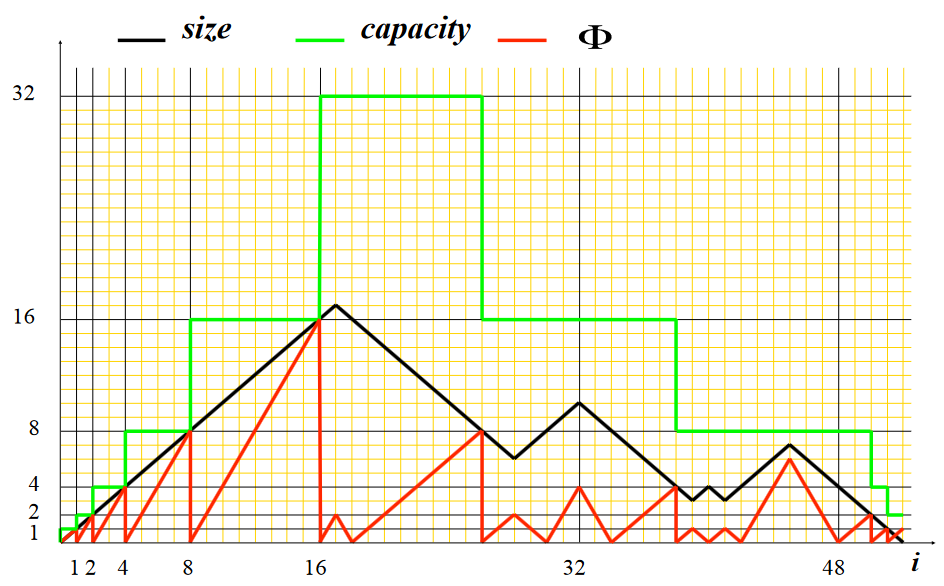
\includegraphics[width=0.5\textwidth]{08/graficoPhiVettore.png}
                \caption{Grafico della funzione di potenziale $\Phi$}
            \end{figure}
    \chapter{Strutture dati speciali}
\thispagestyle{chapterInit}
\section{Code con priorità}
    \subsection{Introduzione}
        Una coda con priorità è una struttura dati astratta, simile ad una coda, in cui ogni elemento ha un valore di priorità associato. Le code con priorità possono essere divise in \textit{Min-Priority Queue} e \textit{Max-Priority Queue}, a seconda che l'elemento con la priorità più bassa o più alta sia quello che viene estratto per primo.
        \subsubsection{Operazioni Permesse}
            Sono permesse le operazioni di inserimento in coda, estrazione dell'elemento con la priorità più alta e la modifica della priorità di un elemento.
        \subsubsection{Specifica}
            \begin{algorithm}
                \caption{\textsc{MinPriorityQueue}}
                \begin{algorithmic}
                    \State \Comment{Crea una coda con capacità massima $n$, vuota}
                    \State \textsc{PriorityQueue}PriorityQueue(\Int $n$)
                    \State \Comment{Restituisce \True se la coda è vuota, \False altrimenti}
                    \State \Bool \Call{IsEmpty}{}
                    \State \Comment{Inserisce l'elemento \Item $x$ con priorità \Int $p$ minima}
                    \State \Item \Call{Min}{}
                    \State \Comment{Restituisce l'elemento con priorità minima}
                    \State \Item \Call{deleteMin}{}
                    \State \Comment{Inserisce l'elemento \Item $x$ con priorità \Int $p$}
                    \State \textsc{PriorityItem} \Call{Insert}{\Item $x$, \Int $p$}
                    \State \Comment{Modifica la priorità dell'elemento \textsc{PriorityItem} $x$ a \Int $p$}
                    \State \Call{DecreaseKey}{\textsc{PriorityItem} $x$, \Int $p$}
                \end{algorithmic}
            \end{algorithm}
        \subsubsection{Reality Check - simulatore \textit{event-drivven}}
            Un esempio di utilizzo delle code con priorità è la simulazione di un sistema \textit{event-driven}, in cui gli eventi con un timestamp associato, sono inseriti in coda con priorità in base al tempo di esecuzione. Ogni evento può generarne altri con timestamp arbitrati. Una coda \textit{min-priority} è perfetta per questo tipo di simulazione in quanto possiamo estrarre l'evento con timestamp minore.
        \subsubsection{Altre applicazioni}
            ALtre applicazioni includono:
                \begin{itemize}
                    \item Algoritmo di Dijkstra
                    \item Codifica di Huffman
                    \item Algoritmo di Prim per gli alberi di copertura di peso minimo
                \end{itemize}
        \subsubsection{Implementazioni}
            Le code con priorità possono essere implementate con diverse strutture dati, di seguito una tabella riassuntiva con le relative complessità:
            \begin{center}
                \begin{tabular}{|c|c|c|c|c|}
                    \hline
                    \textbf{Metodo} & \textbf{Lista/Vettore non ordinato} & \textbf{Vettore ordinato} & \textbf{Lista ordinata} & \textbf{Albero \texttt{RB}} \\
                    \hline
                    min() & $O(n) $ & $O(1)$ & $O(1)$ & $O(\log(n))$ \\
                    \hline
                    deleteMin() & $O(n)$ & $O(n)$ & $O(1)$ & $O(\log(n))$ \\
                    \hline
                    insert() & $O(n)$ & $O(n)$ & $O(n)$ & $O(\log(n))$ \\
                    \hline
                    decreaseKey() & $O(n)$ & $O(\log(n))$ & $O(n)$ & $O(\log(n))$ \\
                    \hline
                \end{tabular}
            \end{center}
            Spesso per la memorizzazione viene usata la memoria \textit{heap} che è una struttura dati speciale che associa i vantaggi di un albero per l'esecuzione ($O(\log(n))$) ed inoltre prende i vantaggi di un vettore.
    \subsection{Vettore \textit{Heap}}
        \subsubsection{Alberi binari}
            \begin{definition}[Albero binario perfetto]
                Si definisce \textbf{albero binario perfetto} un albero binario che rispetti tutte le seguenti condizioni:
                \begin{itemize}
                    \item Tutte le foglie hanno la stessa profondità $h$
                    \item Tutti i nodi interni hanno esattamente grado $2$
                    \item Dato il numero di nodi $n$, ha altezza $h = \left\lfloor\log_2(n)\right\rfloor$
                    \item Data l'altezza $h$, ha $n=2^{h+1}-1$ nodi
                \end{itemize}
            \end{definition}
            \begin{definition}[Albero binario completo]
                Si definisce \textbf{albero binario completo} un albero binario che rispetti tutte le seguenti condizioni:
                \begin{itemize}
                    \item Tutte le foglie hanno profondità $h$ o $h-1$
                    \item Tutti i nodi al livello $h$ sono "accatastati a sinistra"
                    \item Tutti i nodi interni hanno grado $2$ eccetto al più un solo nodo con grado $1$
                    \item Dato il numero di nodi $n$, ha altezza $h = \left\lfloor\log_2(n)\right\rfloor$
                \end{itemize}
            \end{definition}
        \subsubsection{Alberi binari \textit{heap}}
            \begin{definition}[Albero \textit{\{max|min\}-heap}]
                Un \textbf{albero \textit{max-heap}} o \textbf{albero \textit{min-heap}} è un albero binario completo tale che il vettore memorizzato in ogni nodo è maggiore (minore) dei valori memorizzati nei suoi figli.
            \end{definition}
            È utile notare come un albero \textit{max-heap} non impone una relazione di \textbf{ordinamento totale} fra i figli di un nodo questo però non esclude che non sia un \textbf{ordinamento parziale}. Questo è verificabile in quanto si applica: la proprietà di \textbf{riflessività} (Ogni nodo è $\geq $ se stesso), la proprietà di \textbf{anti-simmetria} ($n\geq m \land m\geq n \Rightarrow n=m$) e la proprietà \textbf{transitiva} ($n\geq m \land m\geq p \Rightarrow n\geq p$).\newline
            Un ordinamento parziale è più debole ma più semplice da costruire.
            \paragraph{Vettore \textit{heap}} Un albero \textit{heap} può essere rappresentato tramite un \textbf{vettore \textit{heap}}. In particolare rispettiamo le seguenti regole per la memorizzazione ($A[1\dots n]$):
            \begin{description}
                \item[Radice] $\operatorname{root}()=1$
                \item[Padre nodo $i$] $\operatorname{p}(i)=\left\lfloor\frac{i}{2}\right\rfloor$
                \item[Figlio sinistro nodo $i$] $\operatorname{l}(i)=2i$
                \item[Figlio destro nodo $i$] $\operatorname{r}(i)=2i+1$
            \end{description}
            vengono rispettate le seguenti proprietà: su un albero \textit{max-heap} $A[i]\geq A[\operatorname{l}(i)]$ e $A[i]\geq A[\operatorname{r}(i)]$. Su un albero \textit{min-heap} $A[i]\leq A[\operatorname{l}(i)]$ e $A[i]\leq A[\operatorname{r}(i)]$.
    \subsection{\textit{HeapSort}}
        L'algoritmo \textit{HeapSort} è un algoritmo di ordinamento \textit{in-place} che sfrutta un \textit{max-heap} nel vettore e sposta l'elemento più grande in fondo al vettore. L'algoritmo è composto da due fasi: $\operatorname{heapBuild}()$ e $\operatorname{maxHeapRestore}()$.
        \subsubsection{Funzione $\operatorname{maxHeapRestore}()$}
            L'algoritmo $\operatorname{maxHeapRestore}()$ prende in input un vettore $A$ ed un indice $i$ tale per cui gli alberi binari con radici $\operatorname{l}(i)$ e $\operatorname{r}(i)$ siano \textit{max-heap}. Notare come ciò non esclude il fatto che $A[i]$ sia minore di $A[\operatorname{l}(i)]$ o $A[\operatorname{r}(i)]$. L'algoritmo $\operatorname{maxHeapRestore}()$ ha come obbiettivo quello di modificare \textit{in-place} il vettore $A$ in modo che l'albero con radice $i$ sia un \textit{max-heap}.
            
            \begin{algorithm}
                \caption{\textsc{maxHeapRestore}(\Item[] $A$, \Int $i$, \Int $dim$)}
                \begin{algorithmic}
                    \State \Int $max \gets i$
                    \If {$\operatorname{l}(i) \leq \text{dim} \And A[\operatorname{l}(i)] > A[max]$}
                        \State \Int $max \gets \operatorname{l}(i)$
                    \EndIf
                    \If {$\operatorname{r}(i) \leq \text{dim} \And A[\operatorname{r}(i)] > A[max]$}
                        \State \Int $max \gets \operatorname{r}(i)$
                    \EndIf
                    \If {$max \neq i$}
                        \State \Call{swap}{$A$, $i$, $max$}
                        \State \Call{maxHeapRestore}{$A$, $max$, $dim$}
                    \EndIf
                \end{algorithmic}
            \end{algorithm}
            \paragraph{Complessità}
                La complessità dell'algoritmo $\operatorname{maxHeapRestore}()$ dove, ad ogni chiamata vengono eseguiti $O(1)$ confronti, se il nodo $i$ non è il massimo si chiama ricorsivamente $\operatorname{maxHeapRestore}()$ su uno dei due figli, l'esecuzione termina quando si raggiunge una foglia ed l'altezza dell'albero è $\lfloor\log(n)\rfloor$. Allora la complessità è $O(\log(n))$ in quanto il numero massimo di chiamate ricorsive è $T(n)=O(\log(n))$.
            \paragraph{Dimostrazione della correttezza dell'algoritmo}
                \begin{theorem}
                    Al termine dell'esecuzione, l'albero radicato in $A[i]$ rispetta la proprietà di \textit{max-heap}.
                \end{theorem}
                \begin{proof}
                    La dimostrazione è per induzione sull'altezza $h$ dell'albero:\newline
                    \textbf{Base} ($h=0$): l'albero è una foglia e rispetta la proprietà di \textit{max-heap}.\newline
                    \textbf{Induzione} ($\forall i\leq h \rightarrow A[i]$ albero radicato rispetta la proprietà di \textit{max-heap}): Si distinguono 2 casi:
                    \begin{itemize}
                        \item $A[i]\geq [A[\operatorname{l}(i)]$ e $A[i]\geq A[\operatorname{r}(i)]$: l'albero radicato in $A[i]$ rispetta la proprietà di \textit{max-heap}
                        \item $A[i] < A[\operatorname{l}(i)]$ e $A[i] > A[\operatorname{r}(i)]$: si scambia $A[i]$ con $A[\operatorname{l}(i)]$ dopo lo scambio siamo sicuri che $A[i] \geq A[\operatorname{l}(i)], A[i] \geq A[\operatorname{r}(i)]$ allora il sotto-albero $A[\operatorname{r}(i)]$ è inalterato e rispetta la proprietà \textit{heap}, il sotto-albero $A[\operatorname{l}(i)]$ potrebbe non rispettare la proprietà \textit{heap} e quindi si chiama ricorsivamente $\operatorname{maxHeapRestore}()$ su $A[\operatorname{l}(i)]$, questo ha altezza minore di $h$ e quindi dopo la chiamata rispetta la proprietà di \textit{max-heap}.
                        \item Il caso simmetrico si dimostra in modo analogo.
                    \end{itemize}
                    Per il principio di induzione, il corretto funzionamento dell'algoritmo è dimostrato.
                \end{proof}
        \subsubsection{Funzione $\operatorname{heapBuild}()$}
            Il principio di funzionamento dell'algoritmo $\operatorname{heapBuild}()$ è così descrivibile: a partire da un vettore $A[1\dots n]$ da ordinare, dove tutti i nodi $A\left[\left\lfloor \frac{n}2 \right\rfloor+1\dots n\right]$ sono foglie dell'albero e quindi \textit{heap} contenenti $1$ elemento. La procedura $\operatorname{heapBuild}()$ attraversa i nodi restanti da $\left\lfloor \frac{n}2 \right\rfloor$ a $1$ ed esegue $\operatorname{maxHeapRestore}()$ su ogni nodo.
            
            \begin{algorithm}
                \caption{\textsc{heapBuild}(\Item[] $A$, \Int $n$)}
                \begin{algorithmic}
                    \For{$i \gets \left\lfloor \frac{n}{2} \right\rfloor$ \textbf{to} $1$}
                        \State \Call{maxHeapRestore}{$A$, $i$, $n$}
                    \EndFor
                \end{algorithmic}
            \end{algorithm}
            \begin{proof}
                Quando viene eseguito l'algoritmo $\operatorname{heapBuild}()$ si ha che all'inizio di ogni interazione del ciclo \texttt{for} i nodi $[i+1\dots n]$ sono radice di un \textit{heap}.\newline
                All'inizio del ciclo "prendiamo" $i = \lfloor \frac{n}2\rfloor$, supponendo che $\lfloor \frac{n}2\rfloor + 1$ non sia una foglia, allora ha almeno un figlio sinistro che sarà allocato in posizione $2\lfloor \frac{n}2\rfloor+2$ ovvero $n+1$ o $n+2$ il che è un assurdo in quanto $n$ è la dimensione massima del nostro vettore. Allora $\lfloor \frac{n}2\rfloor + 1$ è una foglia e quindi un \textit{heap} di un solo elemento.\newline
                Possiamo applicare l'algoritmo $\operatorname{maxHeapRestore}()$ sul nodo $i$ in quanto $2i<2i+1\leq n$ e questi sono entrambi radici di un \textit{heap}. Quando l'algoritmo termina tutti i nodi $[i\dots n]$ sono radici di un \textit{heap} rendendo il nodo $1$ la radice di un \textit{heap} e quindi $A$ un \textit{heap} completo.
            \end{proof}
            \paragraph{Complessità}
                La complessità dell'algoritmo $\operatorname{heapBuild}()$, data dal numero di chiamate a $\operatorname{maxHeapRestore}()$ è $O(n\log n)$ in quanto il numero di chiamate a $\operatorname{maxHeapRestore}()$ và da $\lfloor\frac{n}2\rfloor$ a $1$ il che anche se minore di $n$ è comunque $O(n)$. Inoltre la complessità di $\operatorname{maxHeapRestore}()$ è $O(\log n)$. Il che porta ad una complessità totale di $O(n\log n)$.
        \subsubsection{Funzione $\operatorname{heapSort}()$}
            Una volta costruito l'\textit{heap} grazie alle funzioni $\operatorname{heapBuild}()$ e $\operatorname{maxHeapRestore}()$ possiamo assembrale l'algoritmo di ordinamento \textit{HeapSort}.
            \paragraph{Principio di funzionamento} \textit{HeapSort} si basa sul fatto che il primo elemento contenga il massimo, viene quindi scambiato con l'ultimo elemento, viene quindi eseguito $\operatorname{maxHeapRestore}()$ sui nodi $[1\dots i-1]$, dove $i$ è un contatore da $n$ a $2$, si ripete il processo fino a che non si arriva a $2$.
            \begin{algorithm}
                \caption{\textsc{heapSort}(\Item[] $A$, \Int $n$)}
                \begin{algorithmic}
                    \State \Call{heapBuild}{$A$, $n$}
                    \For{$i \gets n$ \DownTo $2$}
                        \State \Call{swap}{$A$, $1$, $i$}
                        \State \Call{maxHeapRestore}{$A$, $1$, $i-1$}
                    \EndFor
                \end{algorithmic}
            \end{algorithm}
            \paragraph{Complessità} In quanto l'algoritmo $\operatorname{heapBuild}()$ ha complessità $\Theta(n)$, l'algoritmo $\operatorname{heapMaxRestore}()$ ha complessità $\Theta(\log i)$, allora possiamo esprimere la complessità dell'algoritmo \textit{HeapSort} come: $$
                T(n)=\sum_{i=2}^{n}\log i+\Theta(n)=\Theta(n\log n)
            $$
            Dunque la complessità dell'algoritmo \textit{HeapSort} è $\Theta(n\log n)$.
    \subsection{Implementazione code con priorità}
        Di seguito viene riportata una possibile implementazione di una coda con priorità utilizzando un \textit{min-heap}, e dunque $\operatorname{minHeapRestore}()$.
        \subsubsection{Memorizzazione}
            
            \begin{algorithm}[H]
                \caption{\textsc{PriorityItem}}
                \begin{algorithmic}
                    \State \Int $priority$ \Comment{Priorità}
                    \State \Item $item$ \Comment{Elemento}
                    \State \Int $pos$ \Comment{Posizione nel vettore \textit{heap}}
                \end{algorithmic}
            \end{algorithm}

            \begin{algorithm}[H]
                \caption{$\operatorname{swap}(\textsc{PriorityItem}[] H, \Int i, \Int j)$}
                \begin{algorithmic}
                    \State \textsc{PriorityItem} $temp \gets H[i]$
                    \State $H[i] \gets H[j]$
                    \State $H[j] \gets temp$
                    \State $H[i].pos \gets i$
                    \State $H[j].pos \gets j$
                \end{algorithmic}
            \end{algorithm}
        
        \subsubsection{Inizializzazione}
            \begin{algorithm}[H]
                \caption{\textsc{PriorityQueue}}
                \begin{algorithmic}
                    \State \Int $capacity$ \Comment{Numero massimo di elementi nella coda}
                    \State \Int $dim$ \Comment{Numero di elementi attualmente nella coda}
                    \State \textsc{PriorityItem}[] $H$ \Comment{Vettore heap}
                    \State \textsc{PriorityQueue} \Function{PriorityQueue}{\Int $n$}
                            \State \textsc{PriorityQueue} $t$ = \New \textsc{PriorityQueue}
                            \State $t.capacity \gets n$
                            \State $t.dim \gets 0$
                            \State $t.H \gets \New \textsc{PriorityItem}[1\dots n]$
                            \State \Return $t$
                        \EndFunction
                \end{algorithmic}
            \end{algorithm}
        \subsubsection{Inserimento}
            \begin{algorithm}[H]
                \caption{\textsc{PriorityItem} insert(\Item $x$, \Int $p$)}
                \begin{algorithmic}
                    \State \textbf{precondition} $dim < capacity$
                    \State $dim \gets dim+1$
                    \State $H[dim] = \New \textsc{PriorityItem}$
                    \State $H[dim].value \gets x$
                    \State $H[dim].priority \gets p$
                    \State $H[dim].pos \gets dim$
                    \State \Int $i \gets dim$
                    \While{$i > 1 \And H[i].priority < H[p(i)].priority$}
                        \State \Call{swap}{$H$, $i$, $p(i)$}
                        \State $i \gets p(i)$
                    \EndWhile
                    \State \Return $H[i]$
                \end{algorithmic}
            \end{algorithm}
        \subsubsection{\texttt{minHeapRestore}()}
            \begin{algorithm}[H]
                \caption{minHeapRestore(\textsc{PriorityItem}[] $A$, \Int $i$, \Int $dim$)}
                \begin{algorithmic}
                    \State \Int $min \gets i$
                    \If {$\operatorname{l}(i) \leq \text{dim} \And A[\operatorname{l}(i)].priority < A[min].priority$}
                        \State \Int $min \gets \operatorname{l}(i)$
                    \EndIf
                    \If {$\operatorname{r}(i) \leq \text{dim} \And A[\operatorname{r}(i)].priority < A[min].priority$}
                        \State \Int $min \gets \operatorname{r}(i)$
                    \EndIf
                    \If {$min \neq i$}
                        \State \Call{swap}{$A$, $i$, $min$}
                        \State \Call{minHeapRestore}{$A$, $min$, $dim$}
                    \EndIf
                \end{algorithmic}
            \end{algorithm}
        \subsubsection{Cancellazione e/o Lettura minimo}
            \begin{algorithm}[H]
                \caption{\textsc{Item} deleteMin()}
                \begin{algorithmic}
                    \State \textbf{precondition} $dim > 0$
                    \State \Call{swap}{$H$, $1$, $dim$}
                    \State $dim \gets dim-1$
                    \State \Call{minHeapRestore}{$H$, $1$, $dim$}
                    \State \Return $H[dim+1].value$
                \end{algorithmic}
            \end{algorithm}
            \begin{algorithm}[H]
                \caption{\textsc{Item} min()}
                \begin{algorithmic}
                    \State \textbf{precondition} $dim > 0$
                    \State \Return $H[1].value$
                \end{algorithmic}
            \end{algorithm}
        \subsubsection{Decremento della priorità}
            \begin{algorithm}[H]
                \caption{decrease(\textsc{PriorityItem} $x$, \Int $p$)}
                \begin{algorithmic}
                    \State \textbf{precondition} $p < x.priority$
                    \State $x.priority \gets p$
                    \State \Int $i \gets x.pos$
                    \While{$i > 1 \And H[i].priority < H[p(i)].priority$}
                        \State \Call{swap}{$H$, $i$, $p(i)$}
                        \State $i \gets p(i)$
                    \EndWhile
                \end{algorithmic}
            \end{algorithm}
        \subsubsection{Complessità}
            Da notare come tutte le operazioni che modificano gli \textit{heap} lasciano inalterata la correttezza della struttura dati, questo o lungo un cammino radice-foglia nel caso della funzione \texttt{deleteMin}() o lungo un cammino foglia-radice nel caso delle funzioni \texttt{insert}() e \texttt{decrease}(). In quanto l'altezza è $\lfloor\log n\rfloor$ la complessità di "sistemare" l'\textit{heap} è $O(\log n)$. Da questo possiamo dire che le operazioni sul \textit{heap} seguono la seguente complessità:
            \begin{table}[H]
                \begin{tabular}{|l|l|}
                    \hline
                    \textbf{Operazione} & \textbf{Complessità} \\
                    \hline
                    \texttt{insert}() & $O(\log n)$ \\
                    \hline
                    \texttt{deleteMin}() & $O(\log n)$ \\
                    \hline
                    \texttt{min}() & $\Omega(1)$ \\
                    \hline
                    \texttt{decrease}() & $O(\log n)$ \\
                    \hline
                \end{tabular}
            \end{table}
    \part{Secondo Semestre}
    \chapter{Programmazione Dinamica}

La tecnica della programmazione dinamica, come per la tecnica \textit{divide-et-impera}, è una tecnica di risoluzione di problemi andando ad dividere il problema in più sotto-problemi, questo però con la differenza che nella programmazione dinamica esiste la possibilità che uno o più sotto-problemi siano uguali tra loro, in questo caso si può sfruttare la tecnica della \textit{memorizzazione} per evitare di ricalcolare più volte lo stesso sotto-problema. Idealmente la soluzione a questo problema è quella di memorizzare i risultati dei sotto-problemi in una tabella, in modo da poterli riutilizzare successivamente, e il \textit{lookup} nella tabella deve essere in tempo $O(1)$.

\paragraph{Approccio Generale}
    \begin{figure}[H]
        \centering
        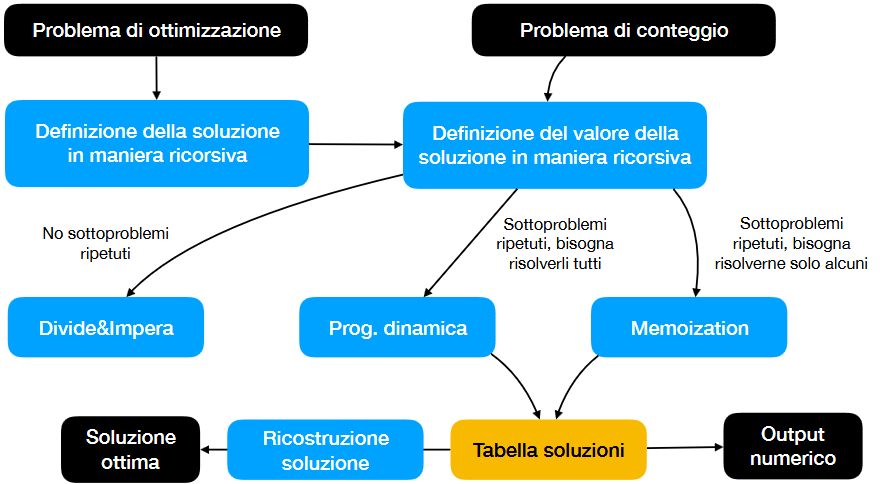
\includegraphics[width=0.6\textwidth]{10/approccioGenerale.png}
        \caption{Grafico dei passi da eseguire sulla base del tipo di problema}
    \end{figure}
    Se il problema è del tipo di ``ottimizzazione'' allora rispetto ai problemi del tipo ``conteggio'' deve essere definita una soluzione in maniera ricorsiva ``di base'' e una funzione di transizione che permetta di passare da un sotto-problema ad un altro. Fatto questo và definito il valore della soluzione in maniera ricorsiva se affrontando il calcolo non vengono rinvenuti sotto-problemi uguali, allora si usa la tecnica \textit{divide-et-impera}, altrimenti usiamo o la programmazione dinamica nel caso nel quale tutti i sotto-problemi vadano risolti, oppure la tecnica della \textit{memorization} nel caso nel quale non tutti i sotto-problemi vadano risolti.\newline
    Negli ultimi due casi non viene fornita immediatamente la soluzione, infatti viene prodotta una ``tabella delle soluzioni'' che nel caso dei problemi di conteggio conterrà il numero di soluzioni, mentre nel caso dei problemi di ottimizzazione bisognerà ricostruire la soluzione a partire dalla tabella delle soluzioni per ottenere la soluzione ottima.

\newpage
\section{Primi Problemi}
    Dopo aver visto l'approccio generale alla programmazione dinamica, vediamo ora alcuni problemi che possono essere risolti con questa tecnica.
    \subsection{Domino}
        Il problema del domino è un problema di conteggio, in cui si vuole contare il numero di modi in cui si possono posizionare $n$ tessere di domino in una scacchiera $2 \times n$ in modo che tutte le celle siano coperte da una tessera di domino. Ad esempio nel caso di $n=4$ allora il numero di modi in cui si possono posizionare le tessere è $5$.
        \begin{figure}[H]
            \centering
            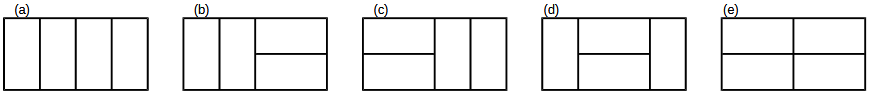
\includegraphics[width=0.8\textwidth]{10/domino.png}
            \caption{Esempio di posizionamento delle tessere di domino per il caso $n=4$}
        \end{figure}
        \subsubsection{Definizione ricorrenza}
            Definiamo una formula ricorsiva $DP[n]$ che definisce il numero di disposizioni possibili con $n$ tessere.
            \paragraph{Casi Base} Per fare ciò dobbiamo stabilire dei ``casi base''. Infatti per $n=0,1$ allora esiste solo $1$ disposizione possibile.
            \paragraph{Casi ricorsivi} Possiamo notare come nel caso nel quale posizionassimo l'ultima tessera in verticale allora le altre precedenti saranno disposte come per il caso $n-1$, mentre se la posiziono in orizzontale allora le precedenti saranno disposte come per il caso $n-2$ in quanto la penultima tessera deve essere posizionata in verticale. Dunque il caso $n$ sarà composto dal caso $n-1$ e dal caso $n-2$.
            \paragraph{Formula Ricorsiva} La formula ricorsiva sarà dunque:
            \begin{equation*}
                DP[n] = \begin{cases}
                    1 & n \leq 1 \\
                    DP[n-1] + DP[n-2] & n > 1
                \end{cases}
            \end{equation*}
            inoltre l'algoritmo ``naive'' per risolvere il problema ha la seguente struttura:
            \begin{algorithm}[H]
                \caption{\Int \texttt{domino1}(\Int $n$)}
                \begin{algorithmic}
                    \If{$n \leq 1$}
                        \State \Return $1$
                    \EndIf
                    \State \Return \texttt{domino1}($n-1$) + \texttt{domino1}($n-2$)
                \end{algorithmic}
            \end{algorithm}
            Questo ha come equazione di ricorrenza:
            $$
                T(n)=\begin{cases}
                    1 & n \leq 1 \\
                    T(n-1) + T(n-2) + 1 & n > 1
                \end{cases}
            $$
            che ha complessità $O(2^n)$.\newline
            Sviluppando l'albero per il caso $n=6$ notiamo come il problema per $n=4$ venga calcolato $2$ volte, per $n=3$ $3$ volte e per $n=2$ $5$ volte, per $n=1$ $8$ volte e per $n=0$ $5$ volte. Questo ci fa capire che questa ripetizione dei calcoli potrebbe essere evitata in qualche modo.
            \paragraph{Tabella $DP$} Per migliorare l'efficienza dell'algoritmo possiamo usare una tabella $DP$ che memorizzi i risultati dei sotto-problemi, in modo da non doverli ricalcolare ogni volta. Oppure in questo caso possiamo usare una interazione \textit{bottom-up} per calcolare i risultati dei sotto-problemi, partendo dai casi base fino ad arrivare al caso $n$.
            \begin{algorithm}[H]
                \caption{\Int \texttt{domino2}(\Int $n$)}
                \begin{algorithmic}
                    \State $DP = \New \Int[0 \ldots n]$
                    \State $DP[0] = DP[1] = 1$
                    \For{$i=2$ \To $n$}
                        \State $DP[i] = DP[i-1] + DP[i-2]$
                    \EndFor
                    \State \Return $DP[n]$
                \end{algorithmic}
            \end{algorithm}
            Questa sicuramente è una soluzione in tempo molto più efficiente, infatti ha complessità $\Theta(n)$, in termini di spazio ha complessità $\Theta(n)$.\newline
            Possiamo migliorare ulteriormente l'algoritmo? In termini di tempo è infattibile in quanto dobbiamo comunque calcolarci \textbf{tutti} i sotto-problemi, ma in termini di spazio per calcolare il valore di $DP[i]$ abbiamo bisogno solo dei valori di $DP[i-1]$ e $DP[i-2]$, gli altri valori non ci servono più.
            Riscriviamo l'algoritmo con l'ultima considerazione:
            \begin{algorithm}[H]
                \caption{\Int \texttt{domino3}(\Int $n$)}
                \begin{algorithmic}
                    \State \Int $DP_0 = 1$
                    \State \Int $DP_1 = 1$
                    \State \Int $DP_2 = 1$
                    \For {$i=2$ \To $n$}
                        \State $DP_0 = DP_1$
                        \State $DP_1 = DP_2$
                        \State $DP_2 = DP_0 + DP_1$
                    \EndFor
                    \State \Return $DP_2$
                \end{algorithmic}
            \end{algorithm}
            Dunque abbiamo ottenuto un algoritmo con complessità $\Theta(n)$ e spazio $\Theta(1)$\dots
            Notiamo però che la serie tende ad un valore che è la sequenza di Fibonacci, la quale ha una crescita più che esponenziale, infatti la formula chiusa per la sequenza di Fibonacci è:
            $$
                F_n = \frac{\left(\frac{1+\sqrt{5}}{2}\right)^n - \left(\frac{1-\sqrt{5}}{2}\right)^n}{\sqrt{5}}
            $$
            Ma allora ``più andiamo avanti più ci servirà del tempo per spostare nello spazio di memoria i valori di $DP$''. Quindi realmente la complessità dell'algoritmo seguendo il modello logaritmico per la complessità spaziale non è $\Theta(1)$ ma $\Theta(n)$. Questo vale anche per le altre soluzioni, infatti:
            \begin{table}[H]
                \centering
                \begin{tabular}{|c|c|c|}
                    \hline
                    \textbf{Funzione} & \textbf{Complessità Spaziale} & \textbf{Complessità Temporale} \\
                    \hline
                    \texttt{domino1} & $O(n^2)$ & $O(n2^n)$ \\
                    \hline
                    \texttt{domino2} & $O(n^2)$ & $O(n^2)$ \\
                    \hline
                    \texttt{domino3} & $O(n)$ & $O(n^2)$ \\
                    \hline
                \end{tabular}
            \end{table}
        \subsection{\textit{Hateville}}
            \textit{Hateville} è un villaggio composto da $n$ case, ed ognuno dei cittadini ($i$) di \textit{Hateville} odia i suoi vicini ($i-1$, $i+1$). Ogni cittadino donerà per la sagra del paese un certo importo, ma non vuole donare se almeno uno dei suoi vicini dona.
            \paragraph{Problema} A noi il compito di calcolare il massimo importo che si può raccogliere, stabilendo, anche, quali sono le case che devono donare.
            \subsubsection{Soluzione} 
                Stabiliamo innanzitutto se è possibile stabilire una definizione ricorsiva del problema, e che se la casa $i$ dona allora la casa $i-1$ e $i+1$ non possono donare.
                \paragraph{Definizione ricorsiva}
                    Sia $HV(i)$ con $i\in [1,n]$ il massimo importo che si può raccogliere se si considerano le case da $1$ a $i$. Allora $HV(n)$ sarà il massimo importo che si può raccogliere.
                \paragraph{Caso ricorsivo} Se non accetto la donazione della casa $i$ allora la casa $i-1$ può donare ed il problema è uguale al problema $HV(i-1)$.
                Se invece accetto la donazione della casa $i$ allora la casa $i-1$ non può donare e dunque la soluzione sarà $HV(i-2) \cup \{i\}$. Dato che noi vogliamo massimizzare il profitto allora sceglieremo $HV(i)=\operatorname{highest}(HV(i-1), HV(i-2) \cup \{i\})$.\footnote{Uso $\operatorname{highest}$ e non $\max$ in quanto sto trattando di insiemi di indici di case e non di valori numerici.}\newline
                Da notare come il seguente approccio non esclude il fatto che ci possano essere più di una soluzione ottima, infatti non nel seguente problema non esiste una soluzione ottimale ma un insieme di soluzioni ottime.\footnote{Ed a questo punto sarebbe cosa buona sapere la differenza tra soluzione ottima e soluzione ottimale.}
                \paragraph{Casi Base} Nel caso in cui $i=0$ allora non esistono case e quindi $HV(0)=\emptyset$, mentre nel caso in cui $i=1$ allora la casa $1$ può donare e quindi $HV(1)=\{1\}$.
                \paragraph{Formula Ricorsiva} La formula ricorsiva sarà dunque:
                $$
                    HV(i)=\begin{cases}
                        \emptyset & i=0 \\
                        \{1\} & i=1 \\
                        \operatorname{highest}(HV(i-1), HV(i-2)\cup \{i\}) & i>1
                    \end{cases}
                $$
            \subsubsection{Dimostrazione della ricorrenza}
                Sia $P_i$ il problema dato dalle prime $i$ case, sia $S_i$ usa delle soluzioni ottime per il problema $P_i$ e sia $||S||=\sum_{j\in S}D[k]$ il totale delle donazione di un qualsiasi insieme $S$ di case.
                \paragraph{Caso 1: $i\not\in S_i$} Allora $S_i$ è una soluzione ottima anche epr $P_{i-1}$ in quanto se così lo fosse stato allora esisterebbe una soluzione $S'_{i-1}$ per il problema $P_{i-1}$ tale che $||S'_{i-1}||>||S_{i}||$ il che non è verificato in quanto $S'_{i-1}$ dovrebbe essere soluzione anche per $P_i$ e che $||S'_{i-1}||>||S_i||$. 
                \paragraph{Caso 2: $i\in S_i$} Allora $S_i\setminus \{i\}$ è una soluzione ottima per il problema $P_{i-2}$ in quanto se così non fosse allora esisterebbe una soluzione $S'_{i-2}$ per il problema $P_{i-2}$ tale che $||S'_{i-2}||>||S_i\setminus \{i\}||$ il che non è verificato in quanto $S'_{i-2}$ dovrebbe essere soluzione anche per $P_i$ e che $||S'_{i-2}\cup \{i\}||>||S_i||$, ma questo è in contraddizione con l'ipotesi che $S_i$ sia soluzione ottima per $P_i$.
            \subsubsection{Passaggio ad algoritmo}
                Una volta definita la formula ricorsiva possiamo passare ad un algoritmo che calcoli il massimo importo che si può raccogliere, ma l'approccio \textit{divide-et-impera} non è il migliore in questo caso, dobbiamo come per il caso del domino calcolare più volte dei sotto-problemi, dunque usiamo la programmazione dinamica.\newline
                Memorizzare il risultato dei sotto-problemi è abbastanza complesso in quanto necessitiamo di memorizzare un insieme di indici. Per la soluzione della prima parte del problema possiamo usare un array $DP$ che memorizzi il massimo importo che si può raccogliere fino alla casa $i$, questo sarà più semplice da implementare ed anche più efficiente. Dunque l'equazione di ricorrenza sarà:
                $$
                    DP[i] = \begin{cases}
                        0 & i=0 \\
                        D[1] & i=1 \\
                        \max(DP[i-1], DP[i-2]+D[i]) & i>1
                    \end{cases}
                $$
                L'algoritmo iterativo corrispondente sarà:
                \begin{algorithm}[H]
                    \caption{\Int \texttt{hateville}(\Int $n$, \Int $D[1 \ldots n]$)}
                    \begin{algorithmic}
                        \State \Int[] $DP = \New \Int[0 \ldots n]$
                        \State $DP[0] = 0$
                        \State $DP[1] = D[1]$
                        \For{$i=2$ \To $n$}
                            \State $DP[i] = \max(DP[i-1], DP[i-2]+D[i])$
                        \EndFor
                        \State \Return $DP[n]$
                    \end{algorithmic}
                \end{algorithm}
                A questo punto abbiamo trovato l'algoritmo per ottenere il valore della soluzione massimale ma non la soluzione in se.
                \paragraph{Ricostruzione della soluzione} Notiamo che il valore di $DP[i]$ deriva da $DP[i]=DP[i-1]$ nel primo caso ed $DP[i]=DP[i-2]+D[i]$ nel secondo, dunque nel primo caso prendiamo la soluzione senza aggiungere nulla, mentre nel secondo aggiungiamo $i$. Dunque possiamo ricostruire la soluzione iterando all'indietro e controllando se il valore di $DP[i]$ deriva da $DP[i-1]$ o da $DP[i-2]+D[i]$.
                \begin{algorithm}[H]
                    \caption{\Set \texttt{hateville}(\Int $n$, \Int $D[1 \ldots n]$)}
                    \begin{algorithmic}
                        \State $[\dots]$
                        \State \Return \Call{solution}{$DP$, $D$, $n$}
                    \end{algorithmic}
                \end{algorithm}
                \begin{algorithm}[H]
                    \caption{\Set \texttt{solution}(\Int[] $DP$, \Int $D[1 \ldots n]$, \Int $i$)}
                    \begin{algorithmic}
                        \If{$i==0$}
                            \State \Return $\emptyset$
                        \ElsIf{$i==1$}
                            \State \Return $\{1\}$
                        \ElsIf{$DP[i]==DP[i-1]$}
                            \State \Return \Call{solution}{$DP$, $D$, $i-1$}
                        \Else
                            \State \Set $sol$ = \Call{solution}{$DP$, $D$, $i-2$}
                            \State $sol$.\Call{insert}{$i$}
                            \State \Return $sol$
                        \EndIf
                    \end{algorithmic}
                \end{algorithm}
                L'algoritmo \texttt{solution()} ha complessità $\Theta(n)$ in merito al tempo, mentre la complessità di \texttt{hateville()} è $\Theta(n)$ in merito al tempo e $\Theta(n)$ in merito allo spazio, se sussiste la necessità di ricostruire la soluzione allora non è possibile ridurre la complessità spaziale.
        \subsection{Zaino (\textit{Knapsack})}
            Il problema dello zaino è un problema di ottimizzazione, in cui si ha uno zaino con una capacità massima $C$ ed lo scopo è quello di riempire lo zaino con oggetti di valore massimo, ma la somma dei pesi degli oggetti non deve superare la capacità dello zaino.\newline
            Si ha quindi in input un vettore $w$ dove $w[i]$ è il peso dell'oggetto $i$ ed un vettore $p$ dove $p[i]$ è il profitto dell'oggetto $i$ ed un intero $C$ che rappresenta la capacità dello zaino. L'algoritmo deve restituire un insieme $S\subseteq \{1,\ldots,n\}$ tale che $w(S)=\sum_{i\in S}w[i]\leq C$ e $\operatorname{argmax}_Sp(S)=\sum_{i\in S}p[i]$.
            \subsubsection{Definizione Ricorsiva}
                Dato lo zaino di capacità $C$ e $n$ oggetti da inserire, definiamo $DP[i][c]$ come il massimo profitto che si può ottenere inserendo i primi $i$ oggetti nello zaino di capacità $c$. Dunque $DP[n][C]$ sarà il massimo profitto che si può ottenere inserendo tutti gli oggetti nello zaino. (Con $i\leq n\land c\leq C$)
                \paragraph{Parte ricorsiva} Come per il precedente problema distinguo se inserire o meno l'oggetto $i$ nello zaino. Se non lo inserisco allora il profitto sarà $DP[i][c]=DP[i-1][c]$, mentre se lo inserisco allora il profitto sarà $DP[i][c]=DP[i-1][c-w[i]]+p[i]$. Anche qui dovrò scegliere il massimo tra i due valori: $DP[i][c]=\max(DP[i-1][c], DP[i-1][c-w[i]]+p[i])$.
                \paragraph{Casi Base} Per stabilire i casi base dobbiamo stabilire il massimo profitto che si può ottenere inserendo $0$ oggetti nello zaino di capacità $c$, ovvero $DP[0][c]=0$, il massimo profitto che si può ottenere inserendo $i$ oggetti nello zaino di capacità $0$, ovvero $DP[i][0]=0$, ed il massimo profitto che si può ottenere inserendo $0$ oggetti nello zaino di capacità negativa $c$, ovvero $DP[0][c]=-\infty$.
                \paragraph{Formula Ricorsiva} La formula ricorsiva sarà dunque:
                $$
                    DP[i][c]=\begin{cases}
                        0 & i=0\lor c=0 \\
                        -\infty & c<0 \\
                        \max(DP[i-1][c], DP[i-1][c-w[i]]+p[i]) & i>0\land c>0
                    \end{cases}
                $$
            \subsubsection{Passaggio ad algoritmo}
                \begin{algorithm}
                    \caption{\Int \texttt{knapsack}(\Int[] $w[1 \ldots n]$, \Int[] $p[1 \ldots n]$, \Int $n$, \Int $C$)}
                    \begin{algorithmic}
                        \State DP = \New \Int[0\dots n][0\dots C]
                        \For{$i=0$ \To $n$}
                            \State $DP[i][0]=0$
                        \EndFor
                        \For{$c=0$ \To $C$}
                            \State $DP[0][c]=0$
                        \EndFor
                        \For{$i=1$ \To $n$}
                            \For{$c=1$ \To $C$}
                                \If{$w[i]\leq c$}
                                    \State $DP[i][c]=\max(DP[i-1][c], DP[i-1][c-w[i]]+p[i])$
                                \Else
                                    \State $DP[i][c]=DP[i-1][c]$
                                \EndIf
                            \EndFor
                        \EndFor
                        \State \Return $DP[n][C]$
                    \end{algorithmic}
                \end{algorithm}
                Visti i due cicli annidati l'algoritmo ha complessità $O(nC)$, però non è un algoritmo polinomiale, questo infatti e pseudo-polinomiale perché sono necessari $k=\lceil\log C\rceil$ \texttt{bit} per rappresentare $C$ e quindi la complessità temporale sarà $O(n2^k)$ 
        \subsection{Zaino con \textit{memorization}}
            Prima di aggiungere la \textit{memorization} all'algoritmo dello zaino, vediamo come possiamo passare ad una versione ricorsiva dell'algoritmo.
            \begin{algorithm}
                \caption{\Int \texttt{knapsack}(\Int[] $w[1 \ldots n]$, \Int[] $p[1 \ldots n]$, \Int $n$, \Int $C$)}
                \begin{algorithmic}
                    \If{$c<0$}
                        \State \Return $-\infty$
                    \ElsIf{$i=0\Or c=0$}
                        \State \Return $0$
                    \Else
                        \State $notTaken = \Call{knapsack}{w, p, i-1, c}$
                        \State $taken = \Call{knapsack}{w, p, i-1, c-w[i]}+p[i]$
                        \State \Return $\max(notTaken, taken)$
                    \EndIf
                \end{algorithmic}
            \end{algorithm}
            La complessità computazionale di \texttt{knapsack()} ricorsiva è $O(2^n)$, in quanto vi è associata la seguente equazione di ricorrenza:
            $$
                T(n)=\begin{cases}
                    1 & n\leq 1\\
                    2T(n-1)+1 & n>1
                \end{cases}
            $$
            In questa soluzione non tutti i sotto-problemi vengono risolti, infatti se $w[i]>c$ allora il problema non viene risolto, ora vediamo come possiamo passare ad una versione con \textit{memorization}.
            \subsubsection{\textit{memorization}}
                Per questo problema uniamo l'approccio ricorsivo di \textit{divide-et-impera} con la tecnica della \textit{memorization}, in modo da evitare di ricalcolare più volte lo stesso sotto-problema.\newline
                Creiamo una tabella $DP$ che inizializzata ad un valore $-1$ ci permetterà di capire se il sotto-problema è già stato risolto o meno. Inoltre la tabella $DP$ sarà di dimensione $n\times C$. Modifichiamo dunque l'algoritmo in modo da inserire la \textit{memorization}.
                \begin{algorithm}
                    \caption{\Int \texttt{knapsack}(\Int[] $w[1 \ldots n]$, \Int[] $p[1 \ldots n]$, \Int $n$, \Int $C$)}
                    \begin{algorithmic}
                        \State DP = \New \Int[0\dots n][0\dots C]
                        \For{$i=0$ \To $n$}
                            \For{$c=0$ \To $C$}
                                \State $DP[i][c]=-1$
                            \EndFor
                        \EndFor
                        \State \Return \Call{knapsackRec}{w, p, n, C, DP}
                    \end{algorithmic}
                \end{algorithm}
                \begin{algorithm}
                    \caption{\Int \texttt{knapsackRec}(\Int[] $w[1 \ldots n]$, \Int[] $p[1 \ldots n]$, \Int $i$, \Int $c$, \Int[][] $DP$)}
                    \begin{algorithmic}
                        \If{$c<0$}
                            \State \Return $-\infty$
                        \ElsIf{$i=0\Or c=0$}
                            \State \Return $0$
                        \ElsIf{$DP[i][c]\neq -1$}
                            \State \Return $DP[i][c]$
                        \Else
                            \State $notTaken = \Call{knapsackRec}{w, p, i-1, c, DP}$
                            \State $taken = \Call{knapsackRec}{w, p, i-1, c-w[i], DP}+p[i]$
                            \State $DP[i][c]=\max(notTaken, taken)$
                            \State \Return $DP[i][c]$
                        \EndIf
                    \end{algorithmic}
                \end{algorithm}
                Questa versione aiuta a ridurre il numero di sotto-problemi che vengono risolti, ma non migliora la complessità computazionale dell'algoritmo, infatti la complessità computazionale in tempo è sempre $O(nC)$.
                \subsubsection{Dizionario/Tabella}
                    Invece di usare una matrice $DP$ possiamo usare un dizionario che memorizzi i risultati dei sotto-problemi, il costo di inizializzazione viene omesso in quanto non necessario, come costo di esecuzione si ha un costo $O(\min(nC, 2^n))$. Questa variante permette di usare solo le caselle necessarie ed evitare calcoli inutili e quindi è più efficiente.
        \subsection{Variante dello Zaino senza limiti}
            In questa variante dello zaino non vi è un limite di quantità per ogni oggetto, ovvero si può prendere un numero illimitato di uno stesso oggetto, dunque. Verifichiamo come l'equazione $DP[i,c]$ cambia rispetto alla variante precedente.
            $$
                DP[i][c]=\begin{cases}
                    0 & i=0\lor c=0 \\
                    -\infty & c<0 \\
                    \max(DP[i-1][c], DP[i\cancel{-1}][c-w[i]]+p[i]) & i>0\land c>0
                \end{cases}
            $$
            La seguente ha come complessità $(nC)$\newline
            Dato che abbiamo eliminato un oggetto dalla formula ricorsiva proviamo ad cerare una tabella con $DP[c]$ rimuovendo l'indice $i$ dalla tabella in quanto non dobbiamo tenere conto di quanti oggetti abbiamo preso, ma solo del profitto massimo che possiamo ottenere con una capacità $c$.
            $$
                DP[c]=\begin{cases}
                    0 & c=0 \\
                    \max_{w[i]\leq c}\{DP[c-w[i]]+p[i]\} & c>0
                \end{cases}
            $$
            Questa formula ha complessità $O(nC)$ e la sua implementazione è la seguente:
            \begin{algorithm}[H]
                \caption{\Int knapsackRec(\Int[] $w[1 \ldots n]$, \Int[] $p[1 \ldots n]$, \Int $n$, \Int $C$)}
                \begin{algorithmic}
                    \State DP = \New \Int[0\dots C]
                    \For{$c=0$ \To $C$}
                        \State $DP[c]=0$
                    \EndFor
                    \For{$c=1$ \To $C$}
                        \State \Int $maxSoFar = 0$ 
                        \For{$i=1$ \To $n$}
                            \If{$w[i]\leq c$}
                                \State \Int $val = $\Call{knapsackRec}{$w, p, i, c-w[i], DP$}+$p[i]$
                                \State $maxSoFar = \max(maxSoFar, val)$
                            \EndIf
                        \EndFor
                        \State $DP[c]=maxSoFar$
                    \EndFor
                    \State \Return $DP[c]$
                \end{algorithmic}
            \end{algorithm}
            Questa ha complessità temporale $T(n)=O(nC)$ infatti nel caso pessimo è necessario riempire ogni cella della tabella $DP$, per riempire ogni singolo valore per $c$ allora è necessario $O(n)$ operazioni.\newline
            In questa versione non possiamo ricostruire la soluzione, ciò in quanto non abbiamo memorizzato gli indici degli oggetti che abbiamo preso, ma solo il profitto massimo che possiamo ottenere con una capacità $c$.
            \subsubsection{Ricostruzione della soluzione}
                Per ricostruire la soluzione possiamo usare un vettore $pos$ che, inizializzato ad $-1$, memorizzi l'indice dell'oggetto che ha portato al profitto massimo per una capacità $c$. In questo modo possiamo ricostruire la soluzione iterando all'indietro e prendendo l'indice dell'oggetto che ha portato al profitto massimo per la capacità $C$. La soluzione cambia come segue:
                \begin{algorithm}[H]
                    \caption{\Int knapsack($\Int[] w[1 \ldots n]$, \Int[] $p[1 \ldots n]$, \Int $n$, \Int $C$)}
                    \begin{algorithmic}
                        \State \Int[] $DP = \New \Int[0\dots C] = \{-1\}$
                        \State \Int[] $pos = \New \Int[0\dots C] = \{-1\}$
                        \State \Call{knapsackRec}{$w, p, n, C, DP, pos$}
                        \State \Return \Call{solution}{$w,C,pos$}
                    \end{algorithmic}
                \end{algorithm}
                \begin{algorithm}[H]
                    \caption{\Int \texttt{knapsackRec}(\Int[] $w[1 \ldots n]$, \Int[] $p[1 \ldots n]$, \Int $i$, \Int $C$, \Int[] $DP$, \Int[] $pos$)}
                    \begin{algorithmic}
                        \If{$C=0$}
                            \State \Return $0$
                        \EndIf
                        \If{$DP[C]<0$}
                            \State $DP[C]=0$
                            \For{$i=1$ \To $n$}
                                \If{$w[i]\leq C$}
                                    \State \Int $val = $\Call{knapsackRec}{$w, p, i, C-w[i], DP, pos$}+$p[i]$
                                    \If{$val>DP[C]$}
                                        \State $DP[C]=val$
                                        \State $pos[C]=i$
                                    \EndIf
                                \EndIf
                            \EndFor
                        \EndIf
                        \State \Return $DP[C]$
                    \end{algorithmic}
                \end{algorithm}
                \begin{algorithm}[H]
                    \caption{\List \texttt{solution}(\Int[] $w$, \Int $C$, \Int[] $pos$)}
                    \begin{algorithmic}
                        \If{$C==0$\Or$pos[C]< 0$}
                            \State \Return \List()
                        \EndIf
                        \State \List $L = \Call{solution}{w, C-w[pos[C]], pos}$
                        \State $L.\Call{insert}{L.\textsc{head}(), pos[C]}$
                        \State \Return $L$
                    \end{algorithmic}
                \end{algorithm}
                Questa lista può contenere un \textbf{multi-insieme} di indici, il che significa che un indice può essere ripetuto più volte, nel caso di capacità $C=0$ allora la lista sarà vuota in quanto la sacca non può contenere oggetti.
                Se invece $pos[c]<0$ allora la capacità $c$ non è stata raggiunta (sacca con capacità pari e pesi dispari) e quindi la lista sarà vuota.
\section{Problemi più complessi su stringhe}
    \subsection{Sotto-sequenza comune massimale}
        Il problema consiste nel trovare quanto due stringe sono simili tra di loro, questo può essere valutato o verificando che una sia sotto-stringa dell'altra oppure tramite delle la ``distanza di \textit{edit}'' tra le due stringhe. In questo caso vediamo come calcolare la lunghezza della sotto-sequenza comune massimale tra due stringhe.
        \subsubsection{Definizione}
            Una sequenza $P$ è una sotto-sequenza di $T$ se $P$ è ottenuto da $T$ rimuovendo uno o più dei suoi elementi, oppure $P$ è definito come sotto-insieme degli indici $\{1,\dots,n\}$ di $T$ tale che $P$ sia una sequenza crescente di indici.
            \begin{definition}[Sotto-sequenza comune]
                Una sotto-sequenza comune tra due sequenze $T$ e $P$ è una sequenza $S$ tale che $S$ è sotto-sequenza di $T$ e di $P$. Scriviamo $X \in\mathcal{CS}(T,U)$
            \end{definition}
            \begin{definition}[Sotto-sequenza massimale]
                Una sotto-sequenza comune massimale tra due sequenze $T$ e $P$ è una sotto-sequenza comune tra $T$ e $P$ tale che non esiste una sotto-sequenza comune più lunga. Scriviamo $X \in\mathcal{\texttt{LCS}}(T,U)$
            \end{definition}
        \subsubsection{Soluzione \textit{brute-force}}
            Una soluzione \textit{brute-force} per il problema è quella di generare tutte le possibili sotto-sequenze di $T$ e di $P$ e di verificare quale sia la più lunga.
            \begin{algorithm}[H]
                \caption{\Int \texttt{LCS}(\Item[] T,\Item U)}
                \begin{algorithmic}
                    \State \Item[] $maxsofar = \Nil$
                    \ForEach{subsequence $X$ of $T$}
                        \If{$X$ is subsequence of $U$}
                            \State $maxsofar = \max(\Call{length}{X}, max)$
                        \EndIf
                    \EndFor
                    \State \Return $maxsofar$
                \end{algorithmic}
            \end{algorithm}
            Data una sequenza $T$ lunga $n$ ci sono $2^n$ sotto-sequenze di $T$, controllare una sequenza è sotto-sequenza costa $O(m+n)$ e quindi la complessità computazionale dell'algoritmo è $\Theta(2^n(m+n))$.
        
        \subsubsection{Descrizione matematica soluzione ottima} 
            \begin{definition}[Prefisso]
                Data una sequenza $T$ composta dai caratteri $t_1t_2\dots t_n$ denotiamo con $T(i)$ il prefisso dato dai primi caratteri tali che: $$
                    T(i)=t_1t_2\dots t_i
                $$
            \end{definition}
            Date due sequenze $T$ e $U$ di lunghezza $n$ e $m$ rispettivamente, denotiamo con $\texttt{LCS}(T(i),U(j))$ che restituisce la \texttt{LCS} dei prefissi $T(i)$ e $U(j)$.
            \paragraph{Casi ricorsivi} Nel caso nel quale l'ultimo carattere di $T$ e $U$ siano uguali allora la \texttt{LCS} sarà uguale alla \texttt{LCS} dei prefissi $T(i-1)$ e $U(j-1)$ più il carattere in comune:
            $$
                LCS(T(i),U(j))=LCS(T(i-1),U(j-1)) \bigoplus t_i
            $$
            Nel caso in cui l'ultimo carattere di $T$ e $U$ siano diversi allora la \texttt{LCS} sarà il massimo tra la \texttt{LCS} di $T(i-1)$ e $U(j)$ e la \texttt{LCS} di $T(i)$ e $U(j-1)$: $$
                LCS(T(i),U(j))=\operatorname{longest}(LCS(T(i-1),U(j)), LCS(T(i),U(j-1)))
            $$
            \paragraph{Casi base}
                Se uno dei due prefissi è vuoto allora la \texttt{LCS} sarà vuota, ovvero $LCS(T(0),U(j))=\emptyset$ e $LCS(T(i),U(0))=\emptyset$.
            \paragraph{Formula Ricorsiva}
                La formula ricorsiva sarà dunque:
                $$
                    LCS(T(i),U(j))=\begin{cases}
                        \emptyset & i=0\lor j=0 \\
                        LCS(T(i-1),U(j-1)) \bigoplus t_i & t_i=u_j \\
                        \operatorname{longest}(LCS(T(i-1),U(j)), LCS(T(i),U(j-1))) & t_i\neq u_j
                    \end{cases}
                $$
        \subsubsection{Sotto-struttura ottima}
            \begin{theorem}[Sotto-struttura ottima]
                Date le due sequenze $T=(t_1,\dots,t_nj)$ e $U=(u_1,\dots,u_m)$ sia $X=(x_1,\dots,x_k)$ una \texttt{LCS} di $T$ e $U$. Allora distinguiamo tre casi:
                \begin{enumerate}
                    \item $t_n=u_m \Rightarrow x_k=t_n=u_m$ e $X_{k-1}\in \mathcal{LCS} (T_{n-1},U_{m-1})$
                    \item $t_n\neq u_m, x_k\neq t_n \Rightarrow X\in \mathcal{LCS}(T_{n-1},U)$
                    \item $t_n\neq u_m, x_k\neq u_m \Rightarrow X\in \mathcal{LCS}(T,U_{m-1})$
                \end{enumerate}
            \end{theorem}
            \paragraph{Dimostrazione punto 1}
                \subparagraph{Parte A}
                Se per assurdo $x_k\neq t_n = u_m$ considerando $Y=Xt_n$ allora $Y\in \mathcal{CS}(T,U)$ e $|Y|>|X|$ il che è in contraddizione con l'ipotesi che $X$ sia una \texttt{LCS} di $T$ e $U$.
                \subparagraph{Parte B} 
                Se per assurdo $X(k-1)\not\in \mathcal{LCS}(T(n-1),U(m-1))$ allora dovrebbe $\exists Y\in\mathcal{LCS}(T(n-1),U(m-1))$ tale che $|Y|>|X(k-1)|$ e quindi $Yt_n\in\mathcal{CS}(T,U)$ e $|Yt_n|>|X(k-1)t_n|=|X|$ il che è in contraddizione con l'ipotesi che $X$ sia una \texttt{LCS} di $T$ e $U$.
            \paragraph{Dimostrazione punto 2 - simmetrico 3}
                Per assurdo se $X\not\in\mathcal{LCS}(T(n-1),U)$ allora $\exists Y\in\mathcal{LCS}(T(n-1),U)$ tale che $|Y|>|X|$ e quindi $Y\in\mathcal{LCS}(T,U)$ e quindi $X\not\in\mathcal{LCS}(T,U)$, il che è in contraddizione con l'ipotesi che $X$ sia una \texttt{LCS} di $T$ e $U$.
        \subsubsection{Riccorrenza soluzione ottimale}
            Avendo quindi stabilito che andiamo in ricorsione sui prefissi delle due stringhe possiamo descrivere l'equazione di ricorrenza come segue:
            $$
                DP[i][j]=\begin{cases}
                    0 & i=0\lor j=0 \\
                    DP[i-1][j-1]+1 & i>0\land j>0\land t_i=u_j \\
                    \max(DP[i-1][j], DP[i][j-1]) & i>0\land j>0\land t_i\neq u_j
                \end{cases}
            $$
            Quindi alla fine $DP[n][m]$ conterrà la lunghezza della sotto-sequenza comune massimale tra $T$ e $U$.
        \subsubsection{Passaggio ad algoritmo}
            \begin{algorithm}[H]
                \caption{\Int \texttt{LCS}(\Item[] $T$, \Item[] $U$)}
                \begin{algorithmic}
                    \State \Int[][] $DP = \New \Int[0\dots n][0\dots m]$
                    \For{$i=0$ \To $n$}
                        \State $DP[i][0]=0$
                    \EndFor
                    \For{$j=0$ \To $m$}
                        \State $DP[0][j]=0$
                    \EndFor
                    \For{$i=1$ \To $n$}
                        \For{$j=1$ \To $m$}
                            \If{$T[i] == U[j]$}
                                \State $DP[i][j]=DP[i-1][j-1]+1$
                            \Else
                                \State $DP[i][j]=\max(DP[i-1][j], DP[i][j-1])$
                            \EndIf
                        \EndFor
                    \EndFor
                    \State \Return $DP[n][m]$
                \end{algorithmic}
            \end{algorithm}
            L'algoritmo ha complessità $O(nm)$ in quanto riempie completamente la tabella $DP$ che ha dimensione $n\times m$.
        \subsubsection{Ricostruzione della soluzione}
            Per ricostruire la soluzione possiamo usare la tabella $DP$ e iterare all'indietro per ricostruire la sotto-sequenza comune massimale.
            \begin{algorithm}[H]
                \caption{\Int \texttt{LCS}(\Item[] $T$, \Item[] $U$)}
                \begin{algorithmic}
                    \State [...] \Comment{Algoritmo per riempire la tabella $DP$}
                    \State \Return \Call{solution}{$DP$, $T$, $U$, $n$, $m$}
                \end{algorithmic}
            \end{algorithm}
            \begin{algorithm}[H]
                \caption{\List \texttt{solution}(\Int[][] $DP$, \Item[] $T$, \Item[] $U$, \Int $i$, \Int $j$)}
                \begin{algorithmic}
                    \If{$i==0 \Or j==0$}
                        \State \Return \List()
                    \EndIf
                    \If{$T[i]==U[j]$}
                        \State \List $L = \Call{solution}{DP, T, U, i-1, j-1}$
                        \State $L.\Call{insert}{L.\textsc{head}(), T[i]}$
                        \State \Return $L$
                    \Else
                        \If{$DP[i-1][j]>DP[i][j-1]$}
                            \State \Return \Call{solution}{DP, T, U, i-1, j}
                        \Else
                            \State \Return \Call{solution}{DP, T, U, i, j-1}
                        \EndIf
                    \EndIf
                \end{algorithmic}
            \end{algorithm}
            Questo algoritmo ripercorre la tabella $DP$ ``all'indietro'' e ricostruisce la sotto-sequenza comune massimale tra $T$ e $U$.\newline
            Il costo della funzione per la ricostruire la soluzione è $O(n+m)$ in quanto la lunghezza della sotto-sequenza comune massimale è $O(n+m)$.\footnote{Esiste un algoritmo più efficiente per il calcolo della lunghezza \texttt{LCS} ma senza la ricostruzione della soluzione andando a conservare nella tabella $DP$ la sola riga precedente, l'algoritmo non è stato riportato}
    \subsection{\textit{String matching} approssimato}
        Il problema dello \textit{string matching} approssimato consiste nel trovare una occorrenza $k$-approssimata di una stringa $P=p_1\dots p_m$ in una stringa $T=t_1\dots p_n$ \footnote{Eventualmente con $n\leq m$}, ovvero una sotto-sequenza $S$ di $T$ tale che $S$ sia una sotto-sequenza di $P$ con al più $k$ errori, i quali possono essere del tipo \textit{mismatch} (un carattere è stato sostituito con un altro), \textit{insertion} (un carattere è stato inserito) e \textit{deletion} (un carattere è stato rimosso).
        \subsubsection{Sottostruttura ottima}
            Sia $DP[0\dots m][0\dots n]$ una tabella di programmazione dinamica tale che $DP[i][j]$ sia il minimo valore $k$ per i quali esiste un'occorrenza $k$-approssimata di $P(i)$ in $T(j)$ che termina in posizione $j$.
            $$
                DP[i][j]=\begin{cases}
                    0 & i=0\land j>0\\
                    i & i\geq0\land j=0\\
                    \min\begin{cases}
                        DP[i-1][j-1] & P[i]=T[j]\\
                        DP[i-1][j-1]+1 & P[i]\neq T[j]\\
                        DP[i][j-1]+1 & \text{inserimento}\\
                        DP[i-1][j]+1 & \text{cancellazione}
                    \end{cases} & i>0\land j>0
                \end{cases}
            $$
            Una volta popolata la tabella $DP$ la soluzione sarà il minimo valore di $DP[m][j]$ per $0\leq j\leq n$. Esempio della ricerca \textit{BAB} in \textit{ABABA}:
            \begin{table}[H]
                \centering
                \begin{tabular}{c |c c c c c c}
                    & A & B & A & B & A & \\
                    \hline
                    $\emptyset$ & 0 & 1 & 2 & 3 & 4 & 5 \\
                    B & 1 & 0 & 1 & 2 & 3 & 4 \\
                    A & 2 & 1 & 0 & 1 & 2 & 3 \\
                    B & 3 & 2 & 1 & 0 & 1 & 2
                \end{tabular}
            \end{table}
            Passando all'algoritmo:
            \begin{algorithm}[H]
                \caption{\Int stringMatching(\Item[] $T$, \Item[] $P$, \Int m, \Int n)}
                \begin{algorithmic}
                    \State \Int[][] $DP = \New \Int[0\dots m][0\dots n]$
                    \For{$j=0$ \To $n$}
                        \State $DP[0][j]=0$
                    \EndFor
                    \For{$i=1$ \To $m$}
                        \State $DP[i][0]=i$
                    \EndFor
                    \For{$i=1$ \To $m$}
                        \For{$j=1$ \To $n$}
                            \State $DP[i][j] = \min\left( DP[i-1][j-1] + \texttt{iff}(P[i]\neq T[j], 1, 0), DP[i][j-1]+1, DP[i-1][j]+1\right)$
                        \EndFor
                    \EndFor
                    \State \Int $pos = 0$
                    \For{$j=0$ \To $n$}
                        \If{$DP[m][j]<DP[m][pos]$}
                            \State $pos=j$
                        \EndIf
                    \EndFor
                    \State \Return $pos$
                \end{algorithmic}
            \end{algorithm}
            \subsection{Prodotto di catena di matrici}
                Il problema del prodotto di catena di matrici consiste nel trovare il modo più efficiente per calcolare il prodotto di $n$ a due a due compatibili matrici. Ricordando che il prodotto di matrici non è commutativo, ovvero $A\cdot B\neq B\cdot A$, ma è associativo, ovvero $(A\cdot B)\cdot C=A\cdot(B\cdot C)$.\newline
                A livello algoritmico vogliamo trovare il modo più efficiente per calcolare il prodotto di $n$ matrici, ovvero vogliamo trovare il modo più efficiente per calcolare il prodotto di $A_1\cdot A_2\cdot A_3\cdot\dots\cdot A_n$ andando ad associare le matrici in modo da minimizzare il numero di moltiplicazioni scalari.
                \subsubsection{Parentesizzazione}
                Una parentesizzazione di $P_{i,j}$ del prodotto $A_i\cdot A_{i+1}\dots A_j$ consiste nella matrice $A_i$ se $i=j$ nel prodotto $A_i\cdot A_{i+1}\dots A_j$ se $i<j$ e in una parentesizzazione di $P_{i,k}$ e di $P_{k+1,j}$ se $i<j$.
                La parentesizzazione ottima di $P_{i,j}$ è la parentesizzazione che minimizza il numero di moltiplicazioni scalari necessarie per calcolare $P_{i,j}$.
                \paragraph{Numero possibile di parentesizzazione} Nel caso $P(n)$ abbiamo $n$ posizioni per \underline{l'ultimo prodotto}. Una volta fissato $k$ abbiamo $P(k)$ parentesizzazioni per $P_{i,k}$ e $P(n-k)$ parentesizzazioni per $P_{k+1,n}$, dunque il numero totale di parentesizzazioni è $P(k)\cdot P(n-k)$, tutto questo và ripetuto per ogni $k$ compreso tra $1$ e $n-1$. Dunque:
                $$
                    P(n)=\begin{cases}
                        1 & n=1\\
                        \sum_{k=1}^{n-1}P(k)\cdot P(n-k) & n>1
                    \end{cases}
                $$
                Dunque provarne tutte le possibili parentesizzazioni ha complessità $\Omega\left(\frac{4^n}{\sqrt{n}}\right)$ il che rende improponibile l'approccio \textit{brute-force}.
            \subsubsection{Parentesizzazione ottima}
                In una parentesizzazione ottima ($A[i\dots j]$) allora esiste un $k$ tale che $A[i\dots j]=A[i\dots k]\cdot A[k+1\dots j]$ e $A[i\dots k]$ e $A[k+1\dots j]$ sono parentesizzazioni ottime di $A[i\dots k]$ e $A[k+1\dots j]$.
                \begin{theorem}
                    Se $P[i\dots j]=P[i\dots k]P[k+1\dots j]$ è una parentesizzazione ottima di $A[i\dots j]$ allora:
                    \begin{itemize}
                        \item $P[i\dots k]$ è una parentesizzazione ottima di $A[i\dots k]$
                        \item $P[k+1\dots j]$ è una parentesizzazione ottima di $A[k+1\dots j]$
                    \end{itemize}
                \end{theorem}
                \begin{proof}
                    Per assurdo se $P[i\dots k]$ non fosse una parentesizzazione ottima di $A[i\dots k]$ allora esisterebbe una parentesizzazione $P'[i\dots k]$ tale che $P'[i\dots k]$ richiede meno moltiplicazioni scalari di $P[i\dots k]$, ma allora $P'[i\dots k]P[k+1\dots j]$ richiederebbe meno moltiplicazioni scalari di $P[i\dots k]P[k+1\dots j]$ il che è in contraddizione con l'ipotesi che $P[i\dots j]$ sia una parentesizzazione ottima di $A[i\dots j]$.
                \end{proof}
            \subsubsection{Valore della soluzione ottima}
                Sia $DP[i][j]$ il minimo numero di moltiplicazioni scalari necessarie per calcolare il prodotto $A_i\cdot A_{i+1}\dots A_j$ allora:
                \paragraph{Caso Base} Se $i=j$ allora $DP[i][j]=0$ in quanto non vi è alcuna moltiplicazione da fare.
                \paragraph{Caso Ricorsivo} Se $i<j$ allora esiste una parentesizzazione ottima $P[i\dots j]$ tale che $P[i\dots j]=P[i\dots k]\cdot P[k+1\dots j]$ allora $DP[i][j] = DP[i][k]+DP[k+1][j]+c_{i-1}\cdot c_k \cdot c_j$ dove $c_i$ è il numero di righe della matrice $A[i]$ e $c_{i-1}$ è il numero di colonne della matrice $A[i-1]$ ed $c_j$ è il numero di colonne della matrice $A[j]$.\newline
                Quindi: $$
                    DP[i][j]=\begin{cases}
                        0 & i=j\\
                        \min_{i\leq k<j}\{DP[i][k]+DP[k+1][j]+c_{i-1}\cdot c_k \cdot c_j\} & i<j
                    \end{cases}
                $$
            \subsubsection{Dalla formula all'algoritmo}
            innanzitutto memorizziamo in un vettore $c[0\dots n]$ la dimensione delle matrici dove $c[0]$ è il numero di righe della prima matrice e $c[i]$ è il numero di colonne della matrice $A[i]$ ed $c[i-1]$ è il numero di righe della matrice $A[i]$. E due indici $i,j$ che partono da $1$ e $n$ rispettivamente.
            \begin{algorithm}[H]
                \caption{\Int recPair(\Int c, \Int i, \Int j)}
                \begin{algorithmic}
                    \If{$i==j$}
                        \State \Return $0$
                    \Else
                        \State $minSoFar = +\infty$
                        \For{\Int $k=i$ \To $j-1$}
                            \State $val = \Call{recPair}{c, i, k}+\Call{recPair}{c, k+1, j}+c[i-1]\cdot c[k]\cdot c[j]$
                            \State $minSoFar = \min(minSoFar, val)$
                        \EndFor
                        \State \Return $minSoFar$
                    \EndIf
                \end{algorithmic}
            \end{algorithm}
            \paragraph{Versione bottom-up} La versione bottom-up dell'algoritmo è la seguente:
            \begin{algorithm}
                \caption{computePair(\Int[] $c$, \Int $n$)}
                \begin{algorithmic}
                    \State \Int[][] $DP = \New \Int[1\dots n][1\dots n]$
                    \For{\Int $i=1$ \To $n$}
                        \State $DP[i][i]=0$
                    \EndFor
                    \State \Int[][] $last = \New \Int[1\dots n][1\dots n]$
                    \For{\Int $h=2$ \To $n$}
                        \For{\Int $i=1$ \To $n-h+1$}
                            \State \Int $j=i+h-1$
                            \State $DP[i][j]=+\infty$
                            \For{\Int $k=i$ \To $j-1$}
                                \State $temp = DP[i][k]+DP[k+1][j]+c[i-1]\cdot c[k]\cdot c[j]$
                                \If{$temp<DP[i][j]$}
                                    \State $DP[i][j]=temp$
                                    \State $last[i][j]=k$
                                \EndIf
                            \EndFor
                        \EndFor
                    \EndFor
                \end{algorithmic}
            \end{algorithm}
    \chapter{Scelta della struttura dati}
In questo capitolo si analizza come può essere eseguita la scelta di una struttura dati rispetto ad un'altra per la risoluzione di uno stesso problema. Si analizzano le strutture dati più comuni e si valutano i pro e i contro di ognuna di esse. Inoltre si analizzano le strutture dati più adatte per la risoluzione di problemi specifici.

\section{Cammini minimi}
    Dato un \textbf{grafo orientato} $G=(V,E)$, un nodo sorgente $s$ ed una funzione peso $w: E \rightarrow \mathbb{R}$, il problema dei cammini minimi consiste nel: ``Dato un cammino $p=<v_1,v_2,\ldots,v_k>$, con $k>1$ e $v_i \in V$, il peso del cammino è dato da $w(p)=\sum_{i=1}^{k-1} w(v_i,v_{i+1})$''. Il problema consiste nel trovare il cammino di peso minimo tra il nodo sorgente $s$ e tutti gli altri nodi del grafo.
    \paragraph{Pesi} Per il seguente problema ci si piò trovare in due casi:
    \begin{itemize}
        \item \textbf{Pesi positivi - positivi/negativi} Se i pesi degli archi sono tutti positivi o se ci sono pesi positivi e negativi, ma non ci sono cicli di peso negativo, allora si può utilizzare l'algoritmo di Dijkstra.
        \item \textbf{Reali - interi} Se i pesi degli archi sono tutti interi o sono reali.
    \end{itemize}
    \paragraph{Sottostruttura ottima} Possono esserci due cammini minimi che condividono uno stesso tratto comune ($A\rightsquigarrow C$) ma non possono convergere in un nodo comune, in quanto l'albero dei cammini minimi è un albero di copertura radicato in $s$ avente un cammino da $s$ a $v$ per ogni $v \in V\setminus\{s\}$.
    \paragraph{Albero di copertura}
        Dato un grafo $G=(V,E)$ non orientato e connesso, un albero di copertura di $G$ è un sottoinsieme di archi $T \subseteq E$ tale che $T$ è un albero, $E_T$ è un sottoinsieme di $E$ e $T$ contiene tutti i nodi di $G$.
    \paragraph{Rappresentazione dell'albero}
        Per rappresentare l'albero usiamo la rappresentazione basata su vettori di padri.
        \begin{algorithm}[H]
            \caption{printPath(\Node $s$, \Node $d$, \Node[] $T$)}
            \begin{algorithmic}
                \If{$d=s$}
                    \State \Call{print}{$s$}
                \ElsIf{$T[d]==\Nil$}
                    \State \Call{print}{``Error''}
                \Else
                    \State \Call{printPath}{$s,T[d],T$}
                    \State \Call{print}{$d$}
                \EndIf
            \end{algorithmic}
        \end{algorithm}
    \subsection{Teorema di Bellman}
        Il teorema di Bellman afferma che una soluzione ammissibile $T$ è \textbf{ottima} se e solo se:
        \begin{align*}
            d[v]=d[u]+w(u,v) \quad& \forall (u,v) \in T\\
            d[v]\leq d[u]+w(u,v) \quad& \forall (u,v) \in E
        \end{align*}
        \begin{proof}
            Sia $T$ una soluzione ottima e siano $(u,v)\in E$ allora se $(u,v)\in T$ allora $d[v]=d[u]+w(u,v)$, altrimenti se $(u,v)\not\in T$ allora $d[v]\leq d[u]+w(u,v)$ altrimenti esisterebbe un altro cammino nel grafo da $u$ a $v$ con peso minore di $d[v]$.\newline
            Sia $T$ per assurdo non sia ottimo, allora esisterebbe una cammino $C$ da $s$ ad un qualunque nodo $u$ con peso minore di $d[u]$, allora esiste un'altro albero $T'$ che contiene $C'$ tale che $w(C')<w(C)$, quindi $T$ non è ottimo.
            Sia $d'$ il vettore delle distanze associato a $T$ poiché $d'[s]=0$ ma $d'[v]<d[v]$ allora esiste un arco $(h,k)\in C'$ tale che $d'[h]=d[h] \land d'[k]<d[k]$. Per costruzione $d'[h]=d[h]$, $d'[k]=d'[h]+w(h,k)$ avendo ipotizzato che $T$ non sia ottimo e che quindi $d[k]\leq d[h]+w(h,k)$, quindi $d'[k]=d'[h]+w(h,k) = d[h]+w(h,k) \geq d[k]$, quindi $d'[k]\geq d[k]$ che è assurdo.
        \end{proof}
        \subsubsection{Algoritmo prototipo}
            \begin{algorithm}[H]
                \caption{$(\Int[], \Int[]) \text{prototipoCamminiMinimi}(\Graph G, \Node s)$}
                \begin{algorithmic}
                    \State \Comment{Inizializza $T$ ad una foresta di copertura composta da nodi isolati}
                    \State \Comment{Inizializza $d$ con sovrastima della distanza ($d[s]=0,d[v]=\infty$)}
                    \While{$\exists (u,v): d[u]+G.\Call{w}{u,v}<d[v]$}
                        \State $d[v]=d[u]+G.\Call{w}{u,v}$
                        \State \Comment{Sostituisci il padre di $v$ con $u$}
                    \EndWhile
                    \State \Return $T,d$
                \end{algorithmic}
            \end{algorithm}
    \subsection{Dijkstra, 1959}
        L'algoritmo di Dijkstra è un algoritmo che nella versione originale veniva usato prt trovare la distanza minima tra soli due nodi e sfrutta il concetto di coda con priorità.
        \subsubsection{Algoritmo}
            \begin{algorithm}[H]
                \caption{shortestPath(\Graph $G$, \Node $s$)}
                \begin{algorithmic}
                    \State \textsc{PriorityQueue} $Q = \textsc{new PriorityQueue}()$
                    \State $Q.\Call{insert}{s,0}$
                    \While{$\not Q.\Call{isEmpty}{}$}
                        \State \Int $u = Q.\Call{extractMin}{}$
                        \State $b[u]=\False$
                        \ForEach{$v \in G.\Call{adj}{u}$}
                            \If{$d[v]>d[u]+G.\Call{w}{u,v}$}
                                \If{$b[v]=\False$}
                                    \State $Q.\Call{insert}{v,d[v]}$
                                    \State $b[v]=\True$
                                \Else
                                    \State $Q.\Call{decreaseKey}{v,d[v]}$
                                \EndIf
                                \State $T[v]=u$
                                \State $d[v]=d[u]+G.\Call{w}{u,v}$
                            \EndIf
                        \EndFor
                    \EndWhile
                \end{algorithmic}
            \end{algorithm}
    \subsubsection{Spiegazione}
        Ogni nodo viene estratto una sola volta ed al momento dell'estrazione la sua distanza è minima, quindi non verrà più modificata. Ciò è dimostrabile per induzione sul numero $k$ di nodi estratti dalla coda. Se $k=1$ allora il nodo estratto è $s$ e la distanza è $0$, se $k>1$ allora quando il nodo estratto è $u$ la distanza $d[u]$ dipende dai nodi $k-1$ già estratti e non dipende dai nodi ancora da estrarre. Quindi $d[u]$ è minima e non verrà più modificata e quindi re-inserita nella coda.
    \subsubsection{Complessità}
        L'algoritmo di Dijkstra nella versione 1959 ha complessità $O(n^2)$, ma con l'uso di una coda con priorità basata su \textit{heap} (\textbf{Jonson 1977}) la complessità diventa $O(m\log n)$, se invece viene usata la \textit{heap} di Fibonacci (\textbf{Fredman-Tarjan 1987}) la complessità diventa $O(m+n\log n)$.
    \subsection{Algoritmo di Bellman-Ford-Moore 1958 - Coda}
        L'algoritmo di Bellman-Ford-Moore è un algoritmo che permette di trovare il cammino minimo tra un nodo sorgente e tutti gli altri nodi del grafo. L'algoritmo è basato su una coda e permette di gestire anche i grafi con cammini di peso negativo.
        \subsubsection{Algoritmo}
            \begin{algorithm}[H]
                \caption{shortestPath(\Graph $G$, \Node $s$)}
                \begin{algorithmic}
                    \State \Queue $Q = \textsc{new Queue}()$
                    \State $Q.\Call{enqueue}{s}$
                    \While{\Not $Q.\Call{isEmpty}{}$}
                        \State \Node $u = Q.\Call{dequeue}{}$
                        \State $b[u]=\False$
                        \ForEach{$v \in G.\Call{adj}{u}$}
                            \If{$d[v]>d[u]+G.\Call{w}{u,v}$}
                                \State $d[v]=d[u]+G.\Call{w}{u,v}$
                                \If{$b[v]=\False$}
                                    \State $Q.\Call{enqueue}{v}$
                                    \State $b[v]=\True$
                                \EndIf
                                \State $T[v]=u$
                            \EndIf
                        \EndFor
                    \EndWhile
                    \State \Return $T,d$
                \end{algorithmic}
            \end{algorithm}
        \subsubsection{Spiegazione}
            Dopo l'inizializzazione nelle prime due righe, si entra nel ciclo principale che estrae un nodo dalla coda e lo esamina. Per ogni nodo adiacente si controlla se la distanza è minore di quella attuale ($+\infty$ se non è stata ancora visitata) e se è minore si aggiorna la distanza e si inserisce il nodo nella coda. Se il nodo è già stato visitato \textbf{e} la distanza è maggiore di quella attuale, allora non si fa nulla.
        \subsubsection{Complessità}
            L'algoritmo ci permette di trovare il cammino minimo tra un nodo sorgente e tutti gli altri nodi del grafo anche nel caso di pesi negativi, tuttavia questo ha un costo computazionale maggiore rispetto all'algoritmo di Dijkstra, infatti un nodo può essere inserito nella coda più di una volta, dato che l'inizializzazione della cosa ha costo $O(1)$, il \textit{dequeue} ha costo $O(1)$ ma viene eseguita $O(n^2)$ volte, quindi la complessità è $O(n^2)$, infine il \textit{enqueue} ha costo $O(1)$ ma viene eseguito $O(nm)$ volte, dunque la complessità totale è $O(nm)$.
    \subsection{Cammini minimi su \texttt{DAG}}
        Dato un grafo orientato aciclico (DAG) $G=(V,E)$, un nodo sorgente $s$ ed una funzione peso $w: E \rightarrow \mathbb{R}$, il problema dei cammini minimi è più semplice in quanto non ci sono cicli e quindi anche in presenza di pesi negativi non incorreremo mai in un ciclo di peso negativo, per semplificare il problema possiamo usare un ordinamento topologico.
        \subsubsection{Algoritmo}
            \begin{algorithm}[H]
                \caption{shortestPath(\Graph $G$, \Node $s$)}
                \begin{algorithmic}
                    \State \Int[] $d = \New \Int[1\dots G.n]$
                    \State \Int[] $T = \New \Int[1\dots G.n]$
                    \ForEach{$u \in G.V$}
                        \State $d[u]=\infty$
                        \State $T[u]=\Nil$
                    \EndFor
                    \State $T[s]=\Nil$
                    \State $d[s]=0$
                    \State \Stack $S = \New \textsc{topSort}(G)$
                    \While{$\Not S.\Call{isEmpty}{}$}
                        \State \Node $u = S.\Call{pop}{}$
                        \ForEach{$v \in G.\Call{adj}{u}$}
                            \If{$d[u]+G.\Call{w}{u,v}<d[v]$}
                                \State $T[v]=u$
                                \State $d[v]=d[u]+G.\Call{w}{u,v}$
                            \EndIf
                        \EndFor
                    \EndWhile
                    \State \Return $T,d$
                \end{algorithmic}
            \end{algorithm}
        \subsubsection{Complessità}
            L'algoritmo ha complessità $O(n+m)$ limitato superiormente dal costo dell'ordinamento topologico.
    \subsection{Recap}
        Riportiamo di seguito una tabella contenete i vari algoritmi per la risoluzione del problema dei cammini minimi con il migliore algoritmo sulla base dei pesi e della struttura del grafo.
        \begin{table}[H]
            \centering
            \begin{tabular}{|c|c|c|}
                \hline
                \textbf{Algoritmo} & \textbf{Complessità} & \textbf{Pesi} \\
                \hline
                \texttt{BFS} & $O(n+m)$ & Senza pesi \\
                Dijkstra & $O(n^2)$ & Positivi, grafi densi \\
                Johnson & $O(m\log n)$ & Positivi, grafi sparsi \\
                Fredman-Tarjan & $O(m+n\log n)$ & Positivi, grafi densi, dimensioni elevate \\
                Bellman-Ford-Moore & $O(nm)$ & Positivi/Negativi \\
                \texttt{DAG} & $O(n+m)$ & Positivi/Negativi (\texttt{DAG}) \\
                \hline
            \end{tabular}
            \caption{Recap cammini minimi}
            \label{tab:recapCamminiMinimi}
        \end{table}
\section{Cammini minimi con sorgente multipla}
    Dato un grafo $G=(V,E)$, un insieme di nodi sorgente $S$ ed una funzione peso $w: E \rightarrow \mathbb{R}$, il problema dei cammini minimi con sorgente multipla consiste nel trovare il cammino di peso minimo tra i nodi sorgente $S$ e tutti gli altri nodi del grafo.\newline
    Intuitivamente possiamo pensare di eseguire l'algoritmo opportuno secondo la tabella precedentemente presentata \ref{tab:recapCamminiMinimi} per ogni nodo sorgente, andando quindi a ottenere le seguenti complessità:
    \begin{table}[H]
        \centering
        \begin{tabular}{|c|c|c|}
            \hline
            \textbf{Input} & \textbf{Algoritmo} & \textbf{Complessità} \\
            \hline
            Pesi positivi, grafi densi & Dijkstra per ogni nodo & $O(n\cdot n^2)=O(n^3)$ \\
            Pesi positivi, grafi sparsi & Johnson per ogni nodo & $O(n\cdot m\log n)$ \\
            Pesi negativi & Bellman-Ford-Moore per ogni nodo & $O(n\cdot nm)=O(n^2m)$ \\
            Pesi negativi grafo denso & Floyd-Warshall & $O(n^3)$ \\
            Pesi negativo grafo sparso & Jonson per sorgenti multiple & $O(n\cdot m\log n)$ \\
            \hline
        \end{tabular}
        \caption{Complessità cammini minimi con sorgente multipla}
    \end{table} 
    \subsection{Floyd-Warshall, 1962}
        L'algoritmo di Floyd-Warshall è un algoritmo che permette di trovare il cammino minimo $k$-vincolato tra due nodi $x$ e $y$ di un grafo $G=(V,E)$, con $k\in\{0,1,\ldots,n\}$ ed il cammino non può passare per i vertici $v_{k+1},\ldots,v_n$ con $x,y$ esclusi da questo vincolo.
        \subsubsection{Distanza $k$-vincolata}
            Denotiamo con $d^k[x][y]$ il costo totale del cammino minimo $k$-vincolato tra $x$ e $y$ se tale cammino esiste, altrimenti $d^k[x][y]=\infty$.
            $$
                d^k[x][y]=\begin{cases}
                    w(p^k_{xy}) & \text{se } p^k_{xy} \text{ esiste}\\
                    \infty & \text{altrimenti}
                \end{cases}
            $$
            La sua formulazione ricorsiva è:
            $$
                d^k[x][y]=\begin{cases}
                    w(x,y) & \text{se } k=0\\
                    \min\{d^{k-1}[x][y],d^{k-1}[x][k]+d^{k-1}[k][y]\} & \text{altrimenti}
                \end{cases}
            $$
            Per la ricostruzione del cammino minimo usiamo una matrice di padri dove la posizione $T[x][y]$ contiene il nodo precedente a $y$ nel cammino minimo tra $x$ e $y$, nel caso $T[x][y]=x$ allora $y$ è adiacente a $x$, altrimenti si deve vedere la cella $T[x][T[x][y]]$ e così via.
        \subsubsection{Algoritmo}
            \begin{algorithm}[H]
                \caption{(\Int[][],\Int[][]) \textsc{FloydWarshall}(\Graph $G$)}
                \begin{algorithmic}
                    \State \Int[][] $d = \New \Int[1\dots G.n][1\dots G.n]$
                    \State \Int[][] $T = \New \Int[1\dots G.n][1\dots G.n]$
                    \ForEach{$u,v \in G.V$}
                        \State $d[u][v]=\infty$
                        \State $T[u][v]=\Nil$
                    \EndFor
                    \ForEach{$u \in G.V$}
                        \ForEach{$v \in G.\Call{adj}{u}$}
                            \State $d[u][v]=G.\Call{w}{u,v}$
                            \State $T[u][v]=u$
                        \EndFor
                    \EndFor
                    \For{$k=1$ \textbf{to} $G.n$}
                        \ForEach{$u \in G.V$}
                            \ForEach{$v \in G.V$}
                                \If{$d[u][v]>d[u][k]+d[k][v]$}
                                    \State $d[u][v]=d[u][k]+d[k][v]$
                                    \State $T[u][v]=T[k][v]$
                                \EndIf
                            \EndFor
                        \EndFor
                    \EndFor
                    \State \Return $(d,T)$
                \end{algorithmic}
            \end{algorithm}
        \subsubsection{Complessità}
            L'algoritmo di Floyd-Warshall ha complessità $O(n^3)$ in quanto una volta inizializzate le matrici $d$ e $T$ si esegue un triplo ciclo annidato per calcolare le distanze minime a partire da $k=1$ fino a $k=n$.
    \subsection{Chiusura transitiva (Algoritmo di Warshall)}
        La chiusura transitiva di un grafo $G=(V,E)$ è un grafo $G'=(V,E')$ orientato tale che $(u,v)\in E'$ se e solo se esiste un cammino da $u$ a $v$ in $G$. L'algoritmo di Warshall permette di calcolare la chiusura transitiva di un grafo in tempo $O(n^3)$ in quanto segue la seguente formula ricorsiva:
        $$
            M^k[x][y]=\begin{cases}
                M[x][y] & \text{se } k=0\\
                M^{k-1}[x][y] \lor (M^{k-1}[x][k] \land M^{k-1}[k][y]) & \text{altrimenti}
            \end{cases}
        $$
    \chapter{Algoritmi \textit{Greedy}}
\label{ch:greedy}

La tecnica \textit{\textbf{greedy}} è una tecnica di progettazione di algoritmi che permette di risolvere problemi di ottimizzazione e problemi di programmazione dinamica, in modo molto efficiente. Gli algoritmi \textit{greedy} sono algoritmi che, tramite una sequenza di scelte ottime locali, costruiscono una soluzione ottima globale. Questa tecnica è molto semplice e veloce, ma se non viene dimostrato il corretto funzionamento dell'algoritmo, non è detto che la soluzione trovata sia la migliore. Inoltre, non tutti i problemi possono essere risolti con questa tecnica.\\
In questo capitolo vedremo come funziona la tecnica \textit{greedy} e come si applica ad alcuni problemi classici.

\section{Primi problemi}
    Andiamo a vedere come si applica la tecnica \textit{greedy} ad alcuni problemi classici.
    \subsection{Insieme indipendente massimale di intervalli}
        Abbiamo visto nella sottosezione \ref{subsec:weightedInterval} - \nameref{subsec:weightedInterval} come trovare l'insieme indipendente massimale di intervalli pesati. Vediamo ora come trovare l'insieme indipendente massimale di intervalli non pesati.
        Come per la soluzione con programmazione dinamica ordiniamo gli intervalli in base alla fine, e definiamo il sotto-problema $S[i\dots j]$ come l'insieme indipendente massimale di intervalli $i\dots j$. Consideriamo inoltre due intervalli $0: b_0=-\infty$ e $n+1: a_{n+1}=\infty$. Ora possiamo suddividere nel problema $S[i\dots j]$, allora esisterà un intervallo $k$ che è presente nella soluzione ottimale di $S[i\dots j]$, allora possiamo dividere il problema in due sotto-problemi $S[i\dots k]$ e $S[k\dots j]$, rispettivamente tutti gli intervalli che finiscono prima di $a_k$ e tutti gli intervalli che iniziano dopo $a_k$. La soluzione ottimale del problema $S[i\dots j]$ conterrà le soluzioni ottimali dei due sotto-problemi $S[i\dots k]$ e $S[k\dots j]$, e le intersezioni $S[i\dots j] \cap S[i\dots k]$ è la soluzione ottimale di $S[i\dots k]$ e $S[k\dots j]\cap S[i\dots j]$ è la soluzione ottimale di $S[k\dots j]$. Quindi possiamo scrivere la formula di ricorrenza:
        $$
            DP[i][j] = \begin{cases}
                0 & S[i\dots j] = \emptyset\\
                \max_{k\in S[i\dots j]}\{DP[i][k] + DP[k][j] + 1\} & S[i\dots j] \neq \emptyset
            \end{cases}
        $$
        Questo porta ad una soluzione $O(n^3)$ ma nel caso degli intervalli pesati siamo riusciti ad ottenere una soluzione $O(n\log n)$, quindi possiamo fare di meglio.\newline
        Consideriamo che non tutti i valori di $k$ vadano presi in considerazione, con questa osservazione possiamo scrivere il seguente teorema:
        \begin{theorem}
            Sia $S[i\dots j]$ un insieme di intervalli ordinati per fine, e sia $m$ l'intervallo in $S[i\dots j]$ con fine minima, allora:
            \begin{enumerate}
                \item Il sotto-problema $S[i\dots m]$ è vuoto
                \item $m$ è presente nella soluzione ottimale di $S[i\dots j]$
            \end{enumerate}
        \end{theorem}
        \begin{proof}
            Parte 1: Per input del problema $a_m < b_m$, per ipotesi $\forall k \in S[i\dots j]: b_m\leq b_k$ e quindi per transitività $\forall k \in S[i\dots j]: a_k \geq b_m$ quindi se nessun intervallo termina prima di $b_m$ allora $S[i\dots m] = \emptyset$.\\
            Parte 2: Supponiamo per assurdo che $m$ non sia presente nella soluzione ($A'[i\dots j]$) ottimale di $S[i\dots j]$, allora esiste un intervallo $m'$ che termina prima di $m$ e che è presente nella soluzione ottimale $A'[i\dots j]$, questo significa che $S[i\dots j] = (A'[i\dots j]-\{m'\})\cup \{m\}$ è una nuova soluzione ottenuta rimuovendo l'intervallo $m'$ e aggiungendo l'intervallo $m$, ma questo è assurdo perché $A[i\dots j]$ è una soluzione ottima che contiene $m$, dato che ha la stessa dimensione di $A'[i\dots j]$ e $A'[i\dots j]$ è una soluzione ottima.
        \end{proof}
        Le conseguenze del teorema appena dimostrato includono il fatto che non tutti gli intervalli sono da prendere in considerazione, ma solo quelli che terminano prima di $m$, ed non è necessario analizzare due sotto-problemi $S[i\dots m]$ e $S[m\dots j]$ ma solo il sotto-problema $S[m\dots j]$. Questo ci permette di scrivere il seguente algoritmo:
        \begin{algorithm}[H]
            \caption{\Set \textsc{maximalIndependentSet}(\Int[] $a$, \Int[] $b$)}
            \begin{algorithmic}
                \State \{ ordina gli intervalli in base alla fine \}
                \State \Set $S \gets \Set()$
                \State $S.\Call{insert}(1)$
                \State \Int $last \gets 1$
                \For{$i \gets 2$ \To $n$}
                    \If{$a[i] \geq b[last]$}
                        \State $S.\Call{insert}(i)$
                        \State $last \gets i$
                    \EndIf
                \EndFor
                \State \Return $S$
            \end{algorithmic}
        \end{algorithm}
        La complessità di questo algoritmo è $O(n)$ nel caso nel quale l'input sia già ordinato, altrimenti $O(n\log n)$ a causa dell'ordinamento da effettuare.
    \subsection{Resto}
        Il problema del resto riguarda la restituzione di un certo importo con il minor numero di monete possibili, date il taglio di queste monete\footnote{supponendo che queste siano infinite} e l'importo da restituire. 
        Con programmazione dinamica possiamo definire una sotto-struttura ottima e risolvere il problema in tempo polinomiale: infatti se $S(i)$ è la risoluzione del problema per il resto $i$, e $A(i)$ è la soluzione ottima per il problema, allora $S(i-t[j])$ è un sotto-problema di $S(i)$, e $A(i) - \{j\}$ è la soluzione ottima per $S(i-t[j])$. Allora possiamo scrivere la formula di ricorrenza:
        $$
            DP[i] = \begin{cases}
                0 & i = 0\\
                \min_{1\leq j \leq n \land t[j] \leq i} DP[i-t[j]] + 1 & i > 0
            \end{cases}
        $$
        la complessità di un algoritmo che risolve il problema del resto con programmazione dinamica è $O(n \cdot R)$ dove $n$ è il numero di tagli di monete e $R$ è l'importo da restituire.
        \subsubsection{Tecnica \textit{greedy}}
            Con la tecnica \textit{greedy} possiamo ipotizzare che una soluzione possibile sia: ``dare il taglio più grande possibile finché o non abbiamo raggiunto l'importo da restituire, o non possiamo dare il taglio più grande, allora passiamo prossimo taglio più piccolo''. Quindi dare resto finché $t[j] \leq R$ e poi risolvere $S(R-t[j])$.
            \paragraph{Algoritmo}
                L'algoritmo corrispondente a questa ipotesi è il seguente:
                \begin{algorithm}[H]
                    \caption{\Int[] \textsc{moneyChange}(\Int[] $t$, \Int $R$)}
                    \begin{algorithmic}
                        \State \Int[] $x \gets \New \Int[1 \ldots n]$
                        \State \{Ordina i tagli in ordine decrescente\}
                        \For{$j \gets 1$ \To $n$}
                            \State $x[i] \gets \left\lfloor\frac{R}{t[j]}\right\rfloor$
                            \State $R \gets R - x[i] \cdot t[j]$
                        \EndFor
                        \State \Return $x$
                    \end{algorithmic}
                \end{algorithm}
        \subsubsection{Dimostrazione $t=[50,10,1]$}
            Sia $x$ una qualunque soluzione ottima, vale dunque:
            $$
                \sum_{i=1}^4 x[i] \cdot t[i] = R \qquad m = \sum_{i=1}^4 x[i] \quad \text{minimo}
            $$
            Sappiamo che $t[k] \cdot x[k] < t[k-1]$ altrimenti basterebbe sostituire un certo numero di monete di taglia $t[k]$ con una moneta di taglia $t[k-1]$ per ottenere una soluzione migliore, nel caso di $t=[50,10,1]$ allora:
            $$
                \begin{aligned}
                    t[2]\cdot x[2] &=&10\cdot x[2] &<t[1]&=50&\Rightarrow x[2]<5\\
                    t[3]\cdot x[3] &=&5\cdot x[3] &<t[2]&=10&\Rightarrow x[3]<2\\
                    t[4]\cdot x[4] &=&1\cdot x[4] &<t[3]&=5&\Rightarrow x[4]<5
                \end{aligned}
            $$
            Sia $m_k$ la somma delle monete di taglio inferiore a $t[k]$, allora:
            $$
                m_k = \sum_{i=k+1}^4 x[i] \cdot t[i]
            $$
            se si può dimostrare che $\forall k: m_k < t[k]$ allora la soluzione ottima è quella calcolata dall'algoritmo \textsc{moneyChange}.
    \subsection{\textit{Scheduling}}
        Prendiamo ora in considerazione il problema dello \textit{scheduling}, che nel modo dei \texttt{SO} è il problema di pianificare quali processi eseguire e in che ordine. Il problema è il seguente: dato un insieme di $n$ processi, ognuno con un tempo di completamento $t_i$, dobbiamo trovare l'ordine di esecuzione dei processi che minimizza il tempo di completamento medio. Il tempo di completamento medio è definito come ``la somma dei tempi di completamento di tutti i processi diviso per il numero di processi''. Ovvero:
        $$
            \frac{1}{n}\sum_{i=1}^n \sum_{j=1}^i t_j
        $$
        Una possibile soluzione è quella di ordinare i processi in base al tempo di completamento crescente, e poi eseguirli in questo ordine. Dunque:
        \begin{theorem}[Scelta \textit{Greedy}]
            Esiste una soluzione ottima di $A$ nella quale il processo col minor tempo di completamento si trova in prima posizione
        \end{theorem}
        \begin{theorem}[Sottostruttura ottima]
            Sia $A$ una soluzione ottima con $n$ processi nella quale il processo con il minor tempo di completamento ($m$) si trova in prima posizione, allora la permutazione dei processi $2\dots n$ in $A$ è una soluzione ottima al sotto-problema dove il processo $m$ è stato rimosso.
        \end{theorem}
        \begin{proof}
            Se consideriamo una permutazione dove il processo $m$, ovvero quello col minor tempo di completamento, non è in prima posizione, allora scambiandolo con il processo in prima posizione otteniamo che:
            \begin{itemize}
                \item Per i processi $A[m+1\dots n]$ il tempo di completamento è lo stesso
                \item Per il processo $A[m]$ il tempo di completamento passa da $\sum_{j=1}^m t_j$ a $t_m$
                \item Per i processi $A[2\dots m-1]$ il tempo di completamento diminuisce di $t_m - t_1$
                \item Per il processo $A[1]$ il tempo di completamento aumenta di $\sum_{j=1}^m t_j$
            \end{itemize}
            Andando a sommare tutte le variazioni otteniamo che il tempo di completamento totale è diminuito, e quindi la soluzione ottenuta è migliore di quella iniziale, dunque la soluzione iniziale non era ottima.
        \end{proof}
    \subsection{Problema dello Zaino Frazionario (Reale)}
        Il problema dello zaino somiglia alla famiglia dei problemi dello zaino affrontati nella sottosezione \ref{subsec:knapsack} - \nameref{subsec:knapsack} e successive, in questa versione del problema abbiamo un insieme di oggetti, ognuno con un peso $w_i$ e un profitto $p_i$, e dobbiamo riempire uno zaino con capacità $C$ in modo da massimizzare il profitto. La differenza con i problemi dello zaino affrontati in precedenza è che possiamo prendere una frazione di un oggetto, e non solo l'oggetto intero. 
        \paragraph{Esempio} Data la seguente tabella:
        \begin{table}[H]
            \centering
            \begin{tabular}{|c|c|c|}
                \hline
                $i$ & $p_i$ & $w_i$\\
                \hline
                1 & 60 \$& 10\\
                2 & 200 \$& 40\\
                3 & 120 \$& 30\\
                \hline
            \end{tabular}
        \end{table}
        e uno zaino con capacità $C=70$ possiamo adottare diverse strategie:
        \subparagraph{Ordinamento profitto decrescente} prendiamo $40/40$ dell'oggetto 2 e $30/30$ dell'oggetto 3, ottenendo un profitto di $200 + 120 = 320\$$.
        \subparagraph{Ordinamento peso crescente} prendiamo $10/10$ dell'oggetto 1, $30/30$ dell'oggetto 3 e $30/40$ dell'oggetto 2, ottenendo un profitto di $60 + 120 + \frac{3}4 \cdot 200 = 330\$$.
        \subparagraph{Ordinamento profitto/peso decrescente} associamo ad ogni oggetto un valore $v_i = \frac{p_i}{w_i}$ e ordiniamo in base a questo valore, ottenendo l'ordine $1 (6\$), 2 (5\$), 3 (4\$)$, prendiamo $10/10$ dell'oggetto 1, $40/40$ dell'oggetto 2 e $20/30$ dell'oggetto 3, ottenendo un profitto di $60 + 200 + \frac{2}3 \cdot 120 = 340\$$.\footnote{In questo caso per lo zaino itero questo approccio non funziona}
        \paragraph{Algoritmo} L'algoritmo per risolvere il problema dello zaino frazionario è il seguente:
        \begin{algorithm}[H]
            \caption{\Float \textsc{fractionalKnapsack}(\Int[] $p$, \Int[] $w$, \Int $C$)}
            \begin{algorithmic}
                \State \Float[] $x = \New \Float[1 \ldots n]$
                \State \{Calcola e ordina i valori di $v_i = \frac{p_i}{w_i}$\}
                \For{\Int $i \gets 1$ \To $n$}
                    \State $x[i] \gets \min(\frac{C}{w[i]}, 1)$
                    \State $C \gets C - x[i] \cdot w[i]$
                \EndFor
                \State \Return $x$
            \end{algorithmic}
        \end{algorithm}
        La complessità di questo algoritmo è $O(n\log n)$ se deve essere effettuato l'ordinamento, altrimenti $O(n)$.
        \subsubsection{Corrtettezza}
            Assumendo che gli oggetti siano stati ordinati per $v_i$ in modo decrescente, e che $x$ sia la soluzione ottima, allora supponendo che $x[1] < \min(\frac{C}{w[1]}, 1) < 1$ ovvero che non abbiamo preso tutto l'oggetto $1$, allora possiamo costruire una nuova soluzione nella quale $x'[1]=\min(\frac{C}{w[1]}, 1)$ e $x'[i]=x[i]$ per $i>1$, ottenendo una soluzione migliore di quella iniziale.
            
    \chapter{\textit{Backtracking}}
\thispagestyle{chapterInit}

Il \textit{backtracking} è una tecnica di ricerca che consente di esplorare in modo sistematico tutte le possibili \textbf{soluzioni ammissibili} di un problema, per trovare una o più soluzioni valide. Una volta trovate tutte le soluzioni ammissibili queste vengono \textbf{valutate} per meglio risolvere i problemi di \textbf{ottimizzazione} che richiedono una soluzione ottimale. 
\begin{definition}[Soluzione ammissibile]
    Dato un problema, una \textbf{soluzione ammissibile} è una soluzione che soddisfa \textbf{un insieme di criteri} definiti per il problema stesso.
\end{definition}
\begin{definition}[Soluzione ottimale]
    Dato un problema, una \textbf{soluzione ottimale} è una soluzione ammissibile che soddisfa \textbf{un insieme di criteri} definiti per il problema stesso e che è \textbf{migliore} rispetto a tutte le altre soluzioni ammissibili.
\end{definition}
\section{\textit{Backtracking} v/s \textit{Brute Force}}
    In alcuni problemi è richiesto esplorare \textbf{l'intero spazio} delle soluzioni ammissibili, questo può essere necessario in questi casi:
    \paragraph{Problemi di enumerazione} Nei problemi di enumerazione è richiesto di trovare tutte le soluzioni ammissibili. Ad esempio, elencare tutte le permutazioni di un insieme di numeri. 
        \subparagraph{Soluzione} Usiamo degli algoritmi di enumerazione
    \paragraph{Problemi di ricerca} Nei problemi di ricerca è richiesto di trovare una o più soluzioni ammissibili. Ad esempio, trovare una sequenza di mosse per il gioco del 15. 
        \subparagraph{Soluzione} Usiamo degli algoritmi enumerazione e ci fermiamo alla prima soluzione trovata.
    \paragraph{Problemi di conteggio} Nei problemi di conteggio è richiesto di contare il numero di soluzioni ammissibili. Ad esempio, contare il numero di possibilità che esistono di esprimere un numero $n$ come somma di $k$ numeri primi.
        \subparagraph{Soluzione} Se il conteggio analitico non è possibile, usiamo degli algoritmi di enumerazione andando a trovare tutte le soluzioni ammissibili e contando il numero di soluzioni trovate.
    \paragraph{Problemi di ottimizzazione} Nei problemi di ottimizzazione è richiesto di trovare la soluzione ammissibile migliore rispetto ad un criterio definito. Trovare il cammino di peso massimo in un grafo dal punto $A$ al punto $B$.
        \subparagraph{Soluzione} Enumeriamo tutti i cammini ammissibili e calcoliamo il peso di ciascuno di essi. La soluzione ottimale è il cammino con peso massimo.
    \subsubsection{Il costo}
        Per tutte queste soluzioni abbiamo dovuto analizzare e calcolare l'intero spazio delle possibili soluzioni che possono anche avere una dimensione super-polinomiale, talvolta questa è l'unica strada per risolvere il problema. Per problemi di dimensione medio-piccoli non è un problema, ma per problemi di dimensione grande il costo di calcolo diventa inaccettabile. Per alcuni di questi problemi non deve essere necessariamente calcolato l'intero spazio delle soluzioni ammissibili, ma solo una parte di esso. 
    \subsubsection{\textit{Backtracking}}
        La filosofia del \textit{backtracking} è quella di esplorare lo spazio delle soluzioni in modo sistematico, se ad un certo punto si scopre che una soluzione non è ammissibile, si torna indietro e si esplora un'altra soluzione. In questo modo si evita di esplorare l'intero spazio delle soluzioni, ma si esplora solo una parte di esso andando ad eliminare le soluzioni che non sono ammissibili.
        \paragraph{Ricorsione} Grazie alla ricorsione possiamo sistematicamente esplorare uno spazio di ricerca ed memorizzare le soluzioni parziali.
        \paragraph{Iterazione} In alcuni casi è possibile utilizzare un approccio iterativo \textit{greedy} per risolvere il problema. Questa strategia può essere utile negli inviluppi convessi o nello \textit{string matching}.
\section{Enumerazione}
    Ora prendiamo in considerazione i problemi di enumerazione, in cui è richiesto di trovare tutte le soluzioni ammissibili. In questo caso il \textit{backtracking} può essere utilizzato per generare tutte le soluzioni ammissibili in modo sistematico.
    \subsubsection{Organizzazione Generale}
        Generalmente una soluzione è rappresenta da un vettore di scelte: $S[1\dots n]$ dove $S[i]$ è la scelta fatta per il passo $i$ presa da un insieme di scelte $C$ \textbf{dipendente} dal problema.
    \subsubsection{Soluzioni Parziali}
        Una soluzione parziale è una soluzione che non è completa, ma sono già state fatte scelte fino ad $i$ ed la nostra soluzione $S[1\dots i-1]$ contiene le scelte fatte fino ad ora. Ora se $S[1\dots i-1]$ è una soluzione ammissibile allora la processiamo assumendo che questa non possa essere estesa. Se invece $S[1\dots i-1]$ non è una soluzione ammissibile, allora calcoliamo l'insieme di scelte $C$ per il passo $i$ e per ogni scelta $c \in C$ proviamo ad estendere la soluzione parziale $S[1\dots i-1]$ con la scelta $c$. Eseguiamo dunque la ricorsione per il passo $i+1$ e continuiamo fino a quando non abbiamo esaurito tutte le scelte. Se una scelta non porta ad una soluzione ammissibile, torniamo indietro e proviamo un'altra scelta. Questo processo continua fino a quando non abbiamo trovato tutte le soluzioni ammissibili.\newline
        Per rappresentare queste scelte è possibile usare un \textbf{albero delle decisioni} che corrisponde allo spazio di ricerca, la radice è la soluzione parziale vuota, per ogni nodo c'è un passo $i$ e per ogni figlio c'è una scelta $c \in C$. Ogni foglia corrisponde ad una soluzione ammissibile.
    \newpage
    \subsection{Sottoinsiemi e Permutazioni}
        \subsubsection{Sottoinsiemi}
            Elencare tutti i sottoinsiemi dell'insieme $S = \{1,\dots, n\}$.\newline
            Sarà dunque possibile scrivere i seguenti algoritmi:
            \begin{algorithm}[H]
                \caption{\textsc{subsetsRec}(\Int $n$, \Int[] $S$, \Int $i$)}
                \begin{algorithmic}
                    \If{$i > n$} \Comment{$S$ ammissibile dopo $n$ scelte}
                        \State \Call{processSolution}{$S, n$}
                    \Else \Comment{Eseguiamo la scelta di prendere o non prendere l'elemento $i$}
                        \State \Set $C \gets \{0, 1\}$
                        \For{$c \in C$}
                            \State $S[i] \gets c$
                            \State \Call{subsetsRec}{$n, S, i + 1$}
                        \EndFor
                    \EndIf
                \end{algorithmic}
            \end{algorithm}
            La chiamata iniziale sarà: 
            \begin{algorithm}[H]
                \caption{\textsc{subsets}(\Int $n$)}
                \begin{algorithmic}
                    \State \Int$[]$ $S \gets \New \Int[1\dots n]$
                    \State \Call{subsetsRec}{$n, S, 1$}
                \end{algorithmic}
            \end{algorithm}
            Ed infine la funzione per processare la soluzione:
            \begin{algorithm}[H]
                \caption{\textsc{processSolution}(\Int[] $S$, \Int $n$)}
                \begin{algorithmic}
                    \State \Call{print}{"\{ "}
                    \For{$i \gets 1$ \textbf{to} $n$}
                        \If{$S[i] = 1$}
                            \State \Call{print}{$i$, " "}
                        \EndIf
                    \EndFor
                    \State \Call{println}{"\}"}
                \end{algorithmic}
            \end{algorithm}
            \paragraph{Complessità} La complessità di questo algoritmo è $\Theta(n\cdot 2^n)$ perché ci sono $2^n$ sottoinsiemi e per ognuno di essi dobbiamo stampare al massimo $n$ elementi. La rappresentazione come albero delle decisioni per $n = 3$ è la seguente:
            \begin{figure}[H]
                \centering
                \begin{tikzpicture}
                    \node(0){$\{\}$}
                        [sibling distance=4cm]
                        child{node{$\{\}$}
                            [sibling distance=2cm]
                            child{node{$\{\}$}
                                [sibling distance=1cm]
                                child{node{$\{\}$}}
                                child{node{$\{3\}$}}
                            }
                            child{node{$\{2\}$}
                                [sibling distance=1cm]
                                child{node{$\{2\}$}}
                                child{node{$\{2,3\}$}}
                            }
                        }
                        child{node{$\{1\}$}
                            [sibling distance=2cm]
                            child{node{$\{1\}$}
                                [sibling distance=1cm]
                                child{node{$\{1\}$}}
                                child{node{$\{1,3\}$}}
                            }
                            child{node{$\{1,2\}$}
                                [sibling distance=1cm]
                                child{node{$\{1,2\}$}}
                                child{node{$\{1,2,3\}$}}
                            }
                        };
                \end{tikzpicture}
                \caption{Albero delle decisioni per $n = 3$}
            \end{figure}
            Esiste la versione iterativa per la risoluzione di questo problema? Si ed il costo è $\Theta(n\cdot 2^n)$
            \begin{algorithm}[H]
                \caption{\textsc{subsetsIter}(\Int $n$)}
                \begin{algorithmic}
                    \For{$j \gets 0$ \To $2^n - 1$}
                        \State \Call{print}{"\{ "}
                        \For{$i \gets 0$ \To $n - 1$}
                            \If{$j \&\& 2^i \neq 0$} \Comment{\textit{Bitwise and}}
                                \State \Call{print}{$i$, " "}
                            \EndIf
                        \EndFor
                        \State \Call{println}{"\}"}
                    \EndFor
                \end{algorithmic}
            \end{algorithm}
            La complessità visto il primo ciclo da $0$ a $2^n - 1$ ed il ciclo interno da $0$ a $n - 1$ è $\Theta(n\cdot 2^n)$.
        \subsubsection{Permutazioni}
            Elencare tutte le permutazioni dell'insieme $S = \{1,\dots, n\}$.\newline
            Sarà dunque possibile scrivere i seguenti algoritmi:
            \begin{algorithm}[H]
                \caption{\textsc{permutationsRec}(\Set $A$, \Item[] $S$, \Int $i$)}
                \begin{algorithmic}
                    \If{$A.\Call{isEmpty}{}$} \Comment{Tutte le scelte sono state fatte}
                        \State \Call{print}{$S$}
                    \Else \Comment{Eseguiamo la scelta di prendere o non prendere l'elemento $i$}
                        \Set $C \gets A.\Call{copy}{}$
                        \ForEach{$c \in C$}
                            \State $S[i] \gets c$
                            \State $A.\Call{remove}{c}$
                            \State \Call{permutationsRec}{$A, S, i + 1$}
                            \State $A.\Call{insert}{c}$
                        \EndFor
                    \EndIf
                \end{algorithmic}
            \end{algorithm}
            La chiamata iniziale sarà:
            \begin{algorithm}[H]
                \caption{\textsc{permutations}(\Set $A$)}
                \begin{algorithmic}
                    \State \Int $n \gets A.\Call{size}()$
                    \State \Item[] $S \gets \New \Item[1\dots n]$
                    \State \Call{permutationsRec}{$A, S, 1$}
                \end{algorithmic}
            \end{algorithm}
            In questo caso l'albero delle decisioni è:
            \begin{figure}[H]
                \centering
                \begin{tikzpicture}
                    \node(0){$\{\}$}
                        [sibling distance=4cm]
                        child{node{$\{A\}$}
                            [sibling distance=2cm]
                            child{node{$\{A, B\}$}
                                [sibling distance=1cm]
                                child{node{$\{A, B, C\}$}}
                            }
                            child{node{$\{A, C\}$}
                                [sibling distance=1cm]
                                child{node{$\{A, C, B\}$}}
                            }
                        }
                        child{node{$\{B\}$}
                            [sibling distance=2cm]
                            child{node{$\{B, A\}$}
                                [sibling distance=1cm]
                                child{node{$\{B, A, C\}$}}
                            }
                            child{node{$\{B, C\}$}
                                [sibling distance=1cm]
                                child{node{$\{B, C, A\}$}}
                            }
                        }
                        child{node{$\{C\}$}
                            [sibling distance=2cm]
                            child{node{$\{C, A\}$}
                                [sibling distance=1cm]
                                child{node{$\{C, A, B\}$}}
                            }
                            child{node{$\{C, B\}$}
                                [sibling distance=1cm]
                                child{node{$\{C, B, A\}$}}
                            }
                        };
                \end{tikzpicture}
                \caption{Albero delle decisioni per $n = 3$}
            \end{figure}
            \paragraph{Complessità} La complessità di questo algoritmo è $\Theta(n\cdot n!)$ in quanto la stampa di ogni permutazione richiede $O(n)$, il costo delle copie richieste per ogni permutazione è $\sum_{1}^{n} O(i) = O(n^2)$ e il numero di foglie è $n!$, dunque il costo totale è $O(n^2 \cdot n!)$.
            \paragraph{Soluzione alternativa} Questo enorme costo può essere ridotto a $\Theta(n \cdot n!)$ se evitiamo di copiare l'insieme $A$ ad ogni passo. In questo caso usando lo stesso vettore andremo a scambiare l'elemento corrente con l'elemento $i$ e eseguiremo la ricorsione. Al termine della ricorsione andremo a scambiare nuovamente l'elemento corrente con l'elemento $i$ per ripristinare lo stato iniziale ed eseguire le chiamate ricorsive ``sorelle'' a quella eseguita.
            \begin{algorithm}[H]
                \caption{\textsc{permutationsRec}(\Item[] $S$, \Int $i$)}
                \begin{algorithmic}
                    \If{$i == 1$} \Comment{Tutte le scelte sono state fatte}
                        \State \Call{println}{$S$}
                    \Else
                        \For{$j \gets 1$ \To $i$}
                            \State \Call{swap}{$S, i, j$}
                            \State \Call{permutationsRec}{$S, i - 1$}
                            \State \Call{swap}{$S, i, j$} \Comment{Ripristina lo stato iniziale}
                        \EndFor
                    \EndIf
                \end{algorithmic}
            \end{algorithm}
            \paragraph{Complessità} La complessità di questo algoritmo è $\Theta(n \cdot n!)$ in quanto la stampa di ogni permutazione richiede $O(n)$ e il numero di foglie è $n!$ e non abbiamo più il costo delle copie richieste per ogni permutazione. Il costo totale è dunque $O(n \cdot n!)$.
        \subsubsection{Schema completo enumerazione}
            Per risolvere i problemi di enumerazione è possibile la seguente ``base'' come algoritmo generale di enumerazione:
            \begin{algorithm}[H]
                \caption{\textsc{enumerate}($\left<\text{dati problema}\right>, \Item[] S, \Int i, \left<\text{dati parziali}\right>$)}
                \begin{algorithmic}
                    \If{\Call{accept}{$\left<\text{dati problema}\right>, S, i, \left<\text{dati parziali}\right>$}} \Comment{Controlla se la soluzione è ammissibile}
                        \State \Call{processSolution}{$\left<\text{dati problema}\right>, S, i, \left<\text{dati parziali}\right>$} \Comment{Processa la soluzione ammissibile}
                    \ElsIf{\Call{reject}{$\left<\text{dati problema}\right>, S, i, \left<\text{dati parziali}\right>$}} \Comment{Controlla se la soluzione è da scartare}
                        \State \Return \Comment{Scarta la soluzione}
                    \Else \Comment{Eseguiamo una scelta}
                        \State \Set $C = \Call{choices}{\left<\text{dati problema}\right>, S, i, \left<\text{dati parziali}\right>}$ \Comment{Calcola le scelte}
                        \ForEach{$c \in C$} \Comment{Per ogni scelta}
                            \State $S[i] \gets c$ \Comment{Aggiorna la soluzione parziale}
                            \State \Call{enumerate}{$\left<\text{dati problema}\right>, S, i + 1, \left<\text{dati parziali}\right>$} \Comment{Esegui la ricorsione}
                        \EndFor
                    \EndIf
                \end{algorithmic}
            \end{algorithm}
            Notiamo come rispetto allo schema generale di \textit{backtracking} abbiamo aggiunto la parte di rifiuto della soluzione. Questa ci permette di scartare delle possibili strade se si scopre che proseguendo con le scelte non si arriverà mai ad una soluzione ammissibile. Nota come nei casi precedenti non possiamo mai scartare una soluzione, ma dobbiamo sempre esplorare l'intero spazio delle soluzioni ammissibili.
        \subsubsection{$k$-Sottoinsiemi}
            Dato un insieme $S$ di $n$ elementi, elencare tutti i sottoinsiemi di $k$ elementi.\newline
            Una prima idea è quella di non prendere in considerazione le soluzioni se alla fine non abbiamo $k$ elementi. In questo caso analizziamo comunque l'intero spazio delle soluzioni ammissibili.\newline
            Un ulteriore miglioramento è quello di scartare tutte le soluzioni che dopo $i$ scelte abbiano lo stesso numero di $k$ elementi o superiori. In questo caso possiamo scartare tutte quelle soluzioni sicuramente inammissibili in quanto avranno un numero di elementi maggiore di $k$.\newline
            Infine possiamo scartare anche le soluzioni parziali che, anche se dalla scelta $i$ in poi prendessero tutti gli elementi, non arriverebbero a $k$ elementi ($n-(i-1)<missing$). In questo caso possiamo scartare tutte quelle soluzioni sicuramente inammissibili in quanto avranno sicuramente un numero di elementi minore di $k$.\newline
            Alla fine dei miglioramenti (\textit{pruning}) il nostro algoritmo sarà:
            \begin{algorithm}[H]
                \caption{\textsc{kSubsetsRec}(\Int $n$, \Int $missing$, \Int[] $S$, \Int $i$)}
                \begin{algorithmic}
                    \If{$missing == 0$} \Comment{Tutte le scelte sono state fatte}
                        \State \Call{processSolution}{$S, i-1$}
                    \ElsIf{$i\leq n \And 0 < missing \leq n - i + 1$} \Comment{Eseguiamo la scelta di prendere o non prendere l'elemento $i$}
                        \ForEach{$c\in\{ 0,1\}$}
                            \State $S[i] \gets c$ \Comment{Aggiorna la soluzione parziale}
                            \State \Call{kSubsetsRec}{$n, missing - c, S, i + 1$} \Comment{Vado avanti con la ricorsione}
                        \EndFor
                    \EndIf
                \end{algorithmic}
            \end{algorithm}
            L'albero delle decisioni per $n = 4$ e $k = 2$ dopo aver applicato il \textit{pruning} è:
            \begin{figure}[H]
                \centering
                \begin{tikzpicture}
                    \node(0){$\{\}$}
                        [sibling distance=8cm]
                        child{node{$\{\}$}
                            [sibling distance=4cm]
                            child{node{$\{\}$}
                                [sibling distance=2cm]
                                child{node{$\{\}$}}
                                child{node{$\{3\}$}
                                    [sibling distance=1cm]
                                    child{node{$\{3\}$}}
                                    child{node{$\{3,4\}$}}
                                }
                            }
                            child{node{$\{2\}$}
                                [sibling distance=2cm]
                                child{node{$\{2\}$}
                                    [sibling distance=1cm]
                                    child{node{$\{2\}$}}
                                    child{node{$\{2,4\}$}}
                                }
                                child{node{$\{2,3\}$}}
                            }
                        }
                        child{node{$\{1\}$}
                            [sibling distance=4cm]
                            child{node{$\{1\}$}
                                [sibling distance=2cm]
                                child{node{$\{1\}$}
                                    [sibling distance=1cm]
                                    child{node{$\{1\}$}}
                                    child{node{$\{1,4\}$}}
                                }
                                child{node{$\{1,2\}$}}
                            }
                            child{node{$\{1,3\}$}}
                        };
                \end{tikzpicture}
                \caption{Albero delle decisioni per $n = 4$ e $k = 2$}
            \end{figure}
        \subsubsection{Ricapitolando}
            Quando specializziamo un algoritmo di \textit{backtracking} per un problema specifico, dobbiamo valutare la possibilità di eseguire del \textit{pruning} per evitare di esplorare soluzioni che non possono mai essere ammissibili. Spesso la versione con \textit{pruning} è più efficiente per valori di $k$ piccoli o grandi, ma non lo sarà altrettanto per valori intermedi, comunque anche per quest'ultimi sarà possibile apprezzare un miglioramento rispetto alla versione senza \textit{pruning}. \newline
            In questo caso non è possibile ottenere lo stesso risultato con un algoritmo iterativo, in quanto non è possibile scartare le soluzioni parziali che non portano a soluzioni ammissibili. 
    \subsection{\textit{Subset sum} - Somma di sottoinsieme}
        Il problema prevede che dato un vettore $A$ contenente $n$ interi positivi, ed un intero positivo $k$ di trovare, se esiste, un sottoinsieme $S\subseteq \{1\dots n\}$ tale che $\sum_{i\in S}a[i]=k$?
        \subsubsection{Analisi del problema}
            Grazie al \textit{backtracking} lo risolveremmo in $O(2^n)$ dovendo analizzare ogni elemento del vettore $A$ e decidere se includerlo o meno nel sottoinsieme $S$.\newline
            In programmazione dinamica può essere risolto in $O(n\cdot k)$, ma non è sempre possibile. Che è pseudo-polinomiale, in quanto il costo dipende da $k$ e da $n$.\newline
            Però per lo scopo del problema a noi non interessano tutte le soluzioni ma solo una, se esiste, quindi nel momento in cui troviamo una soluzione ammissibile possiamo interrompere l'algoritmo.
        \subsubsection{Soluzione}
            Andiamo allora a specializzare l'algoritmo di \textit{backtracking} con \textit{pruning} per evitare di esplorare soluzioni che non possono mai essere ammissibili. 
            \begin{algorithm}[H]
                \caption{\Bool \textsc{subsetSumRec}(\Int[] $A$, \Int $n$, \Int $missing$, \Int[] $S$, \Int $i$)}
                \begin{algorithmic}
                    \If{$missing == 0$} \Comment{Tutte le scelte sono state fatte}
                        \State \Call{processSolution}{$S, i-1$}
                        \State \Return \True
                    \ElsIf{$i>n \Or missing < 0$} \Comment{Controlla se la soluzione è da scartare}
                        \State \Return \False
                    \Else \Comment{Eseguiamo una scelta}
                        \State \Set $C = \{ 0,1\}$
                        \ForEach{$c\in C$}
                            \State $S[i] \gets c$ \Comment{Aggiorna la soluzione parziale}
                            \If{\Call{subsetSumRec}{$A, n, missing - A[i]\cdot c, S, i + 1$}}
                                \State \Return \True
                            \EndIf
                        \EndFor
                        \State \Return \False
                    \EndIf
                \end{algorithmic}
            \end{algorithm}
            Se si potesse avere l'informazione sulle somme cumulative si potrebbe ridurre ancora il costo.
    
    \chapter{\texorpdfstring{Problemi intrattabili - Teoria $\mathbb{NP}$-completi}{Problemi intrattabili - Teoria NP-completi}}
\thispagestyle{chapterInit}

In questo capitolo si andranno ad analizzare problemi il quale tempo di esecuzione non cresce in maniera polinomiale ($O(n^k)$ con $k\in\mathbb{N}$), dunque esistono problemi che per essere risolti richiedono un tempo almeno esponenziale ($\mathbb{EXPTIME}$), alcuni di questi possono essere la valutazione della posizione degli scacchi, il problema delle torri di \textit{Hanoi}. Inoltre esistono problemi che non hanno soluzione, come l'\textit{Halting Problem}.\newline
Tutti i problemi di questa classe hanno in comune il fatto che non è stata dimostrata né l'esistenza, né l'inesistenza di un algoritmo che possa risolverli in tempo polinomiale. Questi problemi sono stati definiti \textbf{intrattabili}.\newline
Prima di prendere in considerazione alcuni esempi, vediamo alcune definizioni:
\begin{definition}[Problema astratto]
    Un \textbf{problema astratto} è una relazione binaria $R\subseteq I\times S$ tra un insieme di istanze $I$ del problema ed un insieme di soluzioni $S$ del problema.\newline
    Esempio: \textit{shortest-path} è un problema astratto, in quanto l'istanza è un grafo $G$ e la soluzione è il cammino più breve tra due nodi $u$ e $v$ ($V,E,u,v$).
\end{definition}
Anche per questa classe di problemi possiamo distinguere diverse categorie:
\begin{definition}
    \item[Ottimizzazione] Data una istanza, trovarne la migliore tramite un criterio specifico
    \item[Ricerca] Data una istanza, trovare una soluzione tra quelle esistenti
    \item[Decisione] Data una istanza, determinare se esiste una soluzione che soddisfi un certo criterio
\end{definition}
I problemi di ottimizzazione contengono infatti i problemi di ricerca e di decisione, in quanto per risolvere un problema di ottimizzazione è necessario prima trovare una soluzione e poi determinare se questa è la migliore. Inoltre i problemi di ottimizzazione e decisione possono essere convertiti l'uno nell'altro, in quanto è possibile trasformare un problema di ottimizzazione in uno di decisione e viceversa. Ad esempio, il problema di ottimizzazione del cammino più breve può essere trasformato in un problema di decisione chiedendo se esiste un cammino di lunghezza minore di $k$.
\section{Riduzioni}
    La \textbf{riduzione polinomiale} viene definita come: presi due problemi decisionali $R_1\subseteq I_1\times\{0,1\}$ e $R_2\subseteq I_2\times\{0,1\}$, allora $R_1$ è riducibile polinomialmente a $R_2$ ($R_1\leq_p R_2$) se esiste una funzione computabile in tempo polinomiale $f:I_1\to I_2$ tale che:
    \begin{itemize}
        \item $f$ è calcolabile in tempo polinomiale
        \item per ogni istanza $x\in I_1$, e ogni soluzione $y\in S_1$ allora $(x,s)\in R_1$ se e solo se $(f(x),s)\in R_2$
    \end{itemize}
    \subsubsection{Colorazione di un grafo}
        Il problema della colorazione di un grafo è un problema di decisione o di ottimizzazione, in cui si chiede se è possibile colorare i vertici di un grafo in modo tale che nessun arco congiunga due vertici dello stesso colore. Dal punto di vista dell'ottimizzazione ci chiediamo quale sia il numero minimo di colori necessari per colorare il grafo, mentre dal punto di vista della decisione ci chiediamo se è possibile colorare il grafo con un numero $k$ di colori.\newline
        Il \textit{sudoku} anche se possa sembrare lontano da questo problema, in realtà è un problema di colorazione di un grafo. Infatti, possiamo rappresentare il \textit{sudoku} come un grafo in cui i vertici rappresentano le celle del \textit{sudoku} e gli archi rappresentano le relazioni tra le celle. In questo modo, il problema di risolvere un \textit{sudoku} diventa un problema di colorazione di un grafo, in cui dobbiamo colorare le celle in modo tale che nessuna cella adiacente abbia lo stesso colore. Per il \textit{sudoku} infatti il problema decisionale sta nel, data una matrice $n^2\times n^2$ determinare se esiste un modo per l'assegnamento di $n^2$ colori a $n^2$ celle in modo tale che nessuna cella adiacente abbia lo stesso colore. Il problema di ottimizzazione invece sta nel determinare il numero minimo di colori necessari per colorare il grafo.
    \subsubsection{Insieme Indipendente}
        Un insieme indipendente è un sottoinsieme di vertici di un grafo non orientato tale che nessun arco congiunga due vertici dello stesso insieme. Dunque: $$
            \forall(x,y)\in E: x\not\in S\land y\not\in S
        $$
        Prendendo in considerazione il seguente grafo:
        \begin{figure}
            \centering
            \begin{tikzpicture}
                \node[draw, circle] (a) at (0,0) {A};
                \node[draw, circle] (b) at (3,0) {B};
                \node[draw, circle] (c) at (0,3) {C};
                \node[draw, circle] (d) at (3,3) {D};
                \node[draw, circle] (e) at (1.5,1.5) {E};
                \draw (a) -- (b);
                \draw (a) -- (c);
                \draw (b) -- (d);
                \draw (c) -- (d);
                \draw (a) -- (e);
                \draw (b) -- (e);
                \draw (c) -- (e);
                \draw (d) -- (e);
            \end{tikzpicture}
            \caption{Grafo con vertici A, B, C, D, E}
        \end{figure}
        In questo grafo al massimo avremmo un insieme indipendente contenente due vertici, ad esempio $\{A,C\}$ o $\{B,D\}$. Se provassimo a prendere tre vertici, ad esempio $\{A,B,C\}$, ci accorgeremmo che esiste un arco che congiunge i vertici $A$ e $B$. 
    \subsubsection{Vertex-Cover}
        La copertura dei vertici è un sottoinsieme di vertici di un grafo non orientato tale che ogni arco del grafo ha almeno un estremo in questo insieme. Dunque: $$
            \forall(x,y)\in E: x\in S\lor y\in S
        $$
        \paragraph{Vertex-Cover, Ottimizzazione} Il problema dell'insieme indipendente è un problema di ottimizzazione, nel quale dato un grafo non orientato $G=(V,E)$, si chiede di restituire la copertura dei vertici di dimensione minima.
        \paragraph{Vertex-Cover, Decisione} Il problema dell'insieme indipendente è un problema di decisione, nel quale dato un grafo non orientato $G=(V,E)$ e un numero intero $k$, si chiede se esiste un insieme indipendente di dimensione al massimo $k$.
    \subsubsection{Riduzione per problewmi duali} 
        Nell'esempio precedente abbiamo visto che il problema dell'insieme indipendente è un problema duale del problema della copertura dei vertici. Infatti, se esiste un insieme indipendente di dimensione $k$, allora esiste una copertura dei vertici di dimensione al massimo $|V|-k$. Dunque, se $S\subseteq V$ è un \textsc{independent set} $\Rightarrow V-S$ è un \textsc{vertex cover}. Dunque possiamo dire che:
        $$
            \textsc{vertex-cover} \leq_p \textsc{independent-set}\\
            \textsc{independent-set} \leq_p \textsc{vertex-cover}
        $$
        Dunque possiamo dire che i due problemi sono duali, e quindi se uno dei due è NP-completo, anche l'altro lo è. Infatti, se esiste un algoritmo polinomiale per risolvere uno dei due problemi, allora esiste un algoritmo polinomiale per risolvere anche l'altro.
    \subsubsection{\texttt{SAT}}
        \texttt{SAT} è un problem a di formule booleane in forma normale congiunta, ovvero dato un insieme $V$ contenente $n$ variabili booleane, ed inoltre:
        \begin{itemize}
            \item un letterale, ovvero una variabile booleana o la sua negazione
            \item una clausola, ovvero una disgiunzione di letterali (separati da $\lor$)
            \item una formula in forma normale congiunta, ovvero una congiunzione di clausole (separate da $\land$)
        \end{itemize}
        Dunque, una formula booleana in forma normale congiunta è una formula booleana che può essere scritta come una congiunzione di clausole, dove ogni clausola è una disgiunzione di letterali. Ad esempio, la formula booleana $(x_1\lor x_2)\land(\neg x_1\lor x_3)$ è in forma normale congiunta, in quanto è una congiunzione di due clausole: $C_1=(x_1\lor x_2)$ e $C_2=(\neg x_1\lor x_3)$. In questo caso abbiamo tre variabili booleane: $x_1$, $x_2$ e $x_3$.\newline
        La soddisfacibilità di una formula booleana in forma normale congiunta è il problema di determinare se esiste un'assegnazione di valori booleani alle variabili in modo tale che la formula sia vera. Ad esempio, per la formula booleana $(x_1\lor x_2)\land(\neg x_1\lor x_3)$, l'assegnazione $x_1=true$, $x_2=false$ e $x_3=true$ rende la formula vera, quindi la formula è soddisfacibile.\newline
        Per risolvere questo problema si potrebbe pensare di ``provare tutte le possibilità'' il che porta ad una complessità non polinomiale, in quanto il numero di possibilità è $2^n$ (dove $n$ è il numero di variabili booleane). 
    \subsubsection{3-SAT}
        Il problema \texttt{3-SAT} è una variante del problema \texttt{SAT}, in cui ogni clausola contiene esattamente tre letterali. Dunque, una formula booleana in forma normale congiunta è in forma normale congiunta 3 se ogni clausola contiene esattamente tre letterali. Ad esempio, la formula booleana $(x_1\lor x_2\lor x_3)\land(\neg x_1\lor x_2\lor x_3)\land(x_1\lor \neg x_2\lor \neg x_3)$ è in forma normale congiunta 3, in quanto è una congiunzione di tre clausole: $C_1=(x_1\lor x_2\lor x_3)$, $C_2=(\neg x_1\lor x_2\lor x_3)$ e $C_3=(x_1\lor \neg x_2\lor \neg x_3)$.
        \paragraph{Obbiettivo} L'obbiettivo è quello di dimostrare che $3-\textsc{sat}\leq_p \textsc{Independent-set} $.
        Possiamo definire il grafo dove per ogni clausola aggiungiamo un trio di nodi collegati da un arco, e per ogni letterale aggiungiamo un arco tra i nodi che rappresentano lo rappresentano e le clausole nel quale questo letterale è presente negato. Dunque la precedente formula può essere rappresentata come:
        \begin{figure}[H]
            \centering
            \begin{tikzpicture}
                \node[draw, circle] (x11) at (0,0) {$x_1$};
                \node[draw, circle] (x21) at (3,0) {$x_2$};
                \node[draw, circle] (x31) at (1.5,1.5) {$x_3$};
                \node[draw, circle] (x12) at (6,0) {$\neg x_1$};
                \node[draw, circle] (x22) at (9,0) {$x_2$};
                \node[draw, circle] (x32) at (7.5,1.5) {$x_3$};
                \node[draw, circle] (x13) at (12,0) {$x_1$};
                \node[draw, circle] (x23) at (15,0) {$\neg x_2$};
                \node[draw, circle] (x33) at (13.5,1.5) {$\neg x_3$};

                \draw[smooth] (x11) -- (x21);
                \draw[smooth] (x11) -- (x31);
                \draw[smooth] (x21) -- (x31);
                \draw[smooth] (x12) -- (x22);
                \draw[smooth] (x12) -- (x32);
                \draw[smooth] (x22) -- (x32);
                \draw[smooth] (x13) -- (x23);
                \draw[smooth] (x13) -- (x33);
                \draw[smooth] (x23) -- (x33);
                \draw[smooth, color=red] (x11) .. controls (1.5,0.5) and (1.5,0.5) .. (x12);
                \draw[smooth, color=red] (x11) .. controls (4.5,0.5) and (4.5,0.5) .. (x13);
                \draw[smooth, color=red] (x22) .. controls (10.5,0.5) and (10.5,0.5) .. (x23);
                \draw[smooth, color=red] (x23) .. controls (14.5,0.5) and (14.5,0.5) .. (x13);
                \draw[smooth, color=red] (x33) .. controls (14.5,0.5) and (14.5,0.5) .. (x32);
                \draw[smooth, color=red] (x33) .. controls (11.5,0.5) and (11.5,0.5) .. (x31);
                % TODO: Finire il grafo

            \end{tikzpicture}
        \end{figure}
        Dunque, se esiste un insieme indipendente di dimensione $k$ allora esiste una soluzione per il problema \texttt{3-SAT} di dimensione $k$. Quindi: $$
            3-\textsc{SAT} \leq_p \textsc{Independent-set}
        $$
        Ma è dimostrabile che per ogni $\texttt{SAT}$ esiste un $3-\texttt{SAT}$, associato, basta spezzare la clausola in $3$ parti, e aggiungere una variabile booleana che le colleghi. Dunque:
        $$
            \texttt{SAT} \leq_p 3-\texttt{SAT}
        $$
        Dunque possiamo dire che:
        $$
            \texttt{SAT} \leq_p \texttt{Independent-set}
        $$
        Dunque possiamo dire che:
        $$
            \texttt{SAT} \leq_p 3-\texttt{SAT} \leq_p \texttt{Independent-set} \leq_p \texttt{Vertex-cover}
        $$
        Dunque risolvendo uno qualsiasi di questi problemi, possiamo risolvere anche gli altri.
\section{\texorpdfstring{Classi $\mathbb{P}$, $\mathbb{PSPACE}$}{Classi P, PSPACE}}
    Dato un problema decisionale $R$ ed un algoritmo $A$ (scritto in forma \textit{Touring}-equivalente), il quale lavora in tempo $f_t(n)$ e spazio $f_s(n)$, diciamo che $A$ risolve $R$ se:
    \begin{itemize}
        \item $A$ è un algoritmo deterministico
        \item $A$ restituisce $s$ su un istanza $x$ di $R$ se e solo se $(x,s)\in R$
    \end{itemize}
    Date le funzioni di cui sopra ($f_t(n)$ e $f_s(n)$) possiamo definiamo le seguenti classi di complessità:
    \begin{itemize}
        \item $\mathbb{TIME}(f(n))$ è la classe dei problemi decisionali risolvibili da un algoritmo deterministico in tempo $O(f_t(n))$
        \item $\mathbb{SPACE}(f(n))$ è la classe dei problemi decisionali risolvibili da un algoritmo deterministico in spazio $O(f_s(n))$
    \end{itemize}
    Definite queste classi di complessità possiamo definire le seguenti classi:
    \begin{itemize}
        \item $\mathbb{P}$ è la classe dei problemi decisionali risolvibili in tempo polinomiale rispetto alla dimensione $n$ dell'input, ovvero: $$
            \mathbb{P}=\bigcup_{c=0}^{\infty}\mathbb{TIME}(n^c)
        $$
        \item $\mathbb{PSPACE}$ è la classe dei problemi decisionali risolvibili in spazio polinomiale rispetto alla dimensione $n$ dell'input, ovvero: $$
            \mathbb{PSPACE}=\bigcup_{c=0}^{\infty}\mathbb{SPACE}(n^c)
        $$
    \end{itemize}
    La classe $P$ è una sottoclasse della classe $PSPACE$, in quanto ogni algoritmo che lavora in tempo polinomiale può essere eseguito in spazio polinomiale. Infatti, se un algoritmo richiede $O(f_t(n))$ tempo per risolvere un problema, allora richiede al massimo $O(f_t(n))$ spazio per memorizzare le informazioni necessarie per la sua esecuzione. Dunque possiamo dire che:
    $$
        \mathbb{P}\subseteq\mathbb{PSPACE}
    $$

\section{\texorpdfstring{Classe $\mathbb{NP}$}{Classe NP}}
    Un certificato è una soluzione che può essere verificata in tempo polinomiale, ovvero un algoritmo che verifica se una soluzione è corretta o meno.
    \begin{definition}[Certificato]
        Dato un problema decisionale $R$ e un'istanza di input $x$, tale che $(x,\textbf{true})\in R$, un \textbf{certificato} è un insieme di informazioni che permette di provare che $x$ è una soluzione valida per il problema $R$.
    \end{definition}
    Un certificato per il problema \texttt{SAT} è una assegnazione di valori booleani alle variabili, che permette di verificare se la formula è soddisfacibile. Ad esempio, per la formula booleana $(x_1\lor x_2)\land(\neg x_1\lor x_3)$, l'assegnazione $x_1=true$, $x_2=false$ e $x_3=true$ è un certificato che dimostra che la formula è soddisfacibile. Questo è un esempio di certificato polinomiale, in quanto la verifica della soddisfacibilità della formula può essere effettuata in tempo polinomiale rispetto al numero di variabili booleane. Esistono però certificati non polinomiali, ovvero certificati che non possono essere verificati in tempo polinomiale. 
    \subsubsection{Certificati non polinomiali}
        \paragraph{\textit{Quantidied Boolean Formula} (\texttt{QBF})}
            Il problema \texttt{QBF} è un problema di decisione che consiste nel determinare se una formula booleana in forma normale congiunta è vera per ogni assegnazione di valori booleani alle variabili. In altre parole, il problema \texttt{QBF} chiede se esiste un'assegnazione di valori booleani alle variabili in modo tale che la formula sia vera per ogni possibile assegnazione.
        \newline
        Dato il problema \texttt{QBF}, trovare un certificato che possa essere verificato in tempo polinomiale.\newline
        Si ritiene che un certificato del genere non possa esistere. Infatti, se esistesse un certificato polinomiale per il problema \texttt{QBF}, allora esisterebbe un algoritmo polinomiale per risolvere il problema \texttt{SAT}.
\section{Problemi \texorpdfstring{$\mathbb{NP}$}{NP}-Completi}
    \begin{definition}[$\mathbb{NP}$-Completo]
        Un problema $R$ è detto \textbf{$\mathbb{NP}$-completo} se:
        \begin{itemize}
            \item $R\in\mathbb{NP}$
            \item $\forall R'\in\mathbb{NP}: R'\leq_p R$
        \end{itemize}
    \end{definition}
    Dunque, un problema è $\mathbb{NP}$-completo se questo è in $\mathbb{NP}$ e ogni problema in $\mathbb{NP}$ è riducibile a questo problema. Dunque, se esiste un algoritmo polinomiale per risolvere un problema $\mathbb{NP}$-completo, allora ogni problema in $\mathbb{NP}$ può essere risolto in tempo polinomiale. Dunque, se esiste un algoritmo polinomiale per risolvere un problema $\mathbb{NP}$-completo, allora $\mathbb{P}=\mathbb{NP}$.
    \subsubsection{Esistono problemi $\mathbb{NP}$-completi?}
        Per fare ciò dovremmo dimostrare che esiste un problema tale per cui ogni problema nella classe $\mathbb{NP}$ è riducibile a questo problema. In precedenza abbiamo visto come
        $$
            \texttt{SAT} \leq_p 3-\texttt{SAT} \leq_p \texttt{Independent-set} \leq_p \texttt{Vertex-cover}
        $$
        Dunque, se esiste un algoritmo polinomiale per risolvere \texttt{Vertex-cover}, allora esiste un algoritmo polinomiale per risolvere anche \texttt{SAT}, ciò non dimostra che \texttt{vertex-cover} è $\mathbb{NP}$-completo, ma per il teorema di \textit{Cook-Levin} possiamo dire che \texttt{SAT} è $\mathbb{NP}$-completo \footnote{\url{https://en.wikipedia.org/wiki/Cook-Levin_theorem}}. Dunque possiamo dire che:
        $$
            \texttt{SAT} \leq_p \texttt{3-SAT} \leq_p \texttt{Independent-set} \leq_p \texttt{Vertex-cover} \leq \texttt{SAT}
        $$
        E dunque ognuno di questi problemi è $\mathbb{NP}$-completo in quanto \texttt{SAT} è $\mathbb{NP}$-completo ed gli altri possono essere usati per ridurre \texttt{SAT} a loro.\newline
        Esistono molti problemi riducibili a \texttt{SAT} oltre a quelli visti, e dunque $\mathbb{NP}$-completi, tra cui:
        \begin{itemize}
            \item \texttt{Clique}
            \item \texttt{Hamiltonian-path}
            \item \texttt{Hamiltonian-cycle}
            \item \texttt{Traveling-salesman}
            \item \texttt{Graph-coloring}
            \item \texttt{Knapsack}
            \item \texttt{Set-cover}
            \item \texttt{Job-scheduling}
        \end{itemize}
        tutti questi hanno una pratica applicazione nel mondo reale, e dunque sono stati studiati a lungo ma non esiste un algoritmo polinomiale per risolverli. Dunque possiamo dire che al momento non esiste un algoritmo polinomiale per risolvere i problemi $\mathbb{NP}$-completi, e dunque non esiste un algoritmo polinomiale per risolvere i problemi in $\mathbb{NP}$.
    \chapter{Tecniche risolutive per problemi intrattabili}

Anche se non è stato dimostrato che i problemi intrattabili ($NP$) siano risolvibili in tempo polinomiale, questi rimangono comunque interessanti e utili. Infatti, esistono tecniche che permettono di affrontare questi problemi, o una loro parte, in modo efficiente. Queste tecniche non garantiscono una soluzione ottimale, ma possono fornire soluzioni approssimate o risolvere casi specifici in tempi accettabili.

\paragraph{A cosa rinunciamo?}
Dato non possiamo avere una soluzione ottimale in tempi polinomiali, dobbiamo rinunciare a qualcosa. Possiamo rinunciare a:
\begin{description}
    \item[Generalità] Possiamo rinunciare a risolvere il problema in modo generale, e limitarci a casi specifici.
    \item[Ottimalità] Possiamo rinunciare a trovare la soluzione ottimale, e limitarci a trovare una soluzione approssimata. In questo caso viene ricavato anche l'errore che si commette.
    \item[Formalità] Possiamo rinunciare a formalizzare il problema, e limitarci a risolvere il problema in modo euristico. Ovvero non formale, usando tecniche come \textit{greedy}, \textit{branch and bound}, \textit{backtracking}, \textit{dynamic programming}, \textit{randomized algorithms} e \textit{approximation algorithms}.
    \item[Efficienza] Possiamo rinunciare a risolvere il problema in modo efficiente, e limitarci a risolvere il problema in modo esatto, ma in tempi esponenziali. 
\end{description}

\section{Algoritmi pseudo-polinomiali}
    Prendiamo in considerazione il seguente problema:
    \subsection{Somma di sottoinsiemi (\textsc{subset-sum})}
        Dati un vettore $A$ contente $N$ numeri interi e un numero intero $k$, determinare se esiste un sottoinsieme di $S\subseteq\{1,\ldots,N\}$ tale che la somma degli elementi di $S$ sia uguale a $\sum_{i\in S} A_i = k$.
        \subsubsection{Programmazione dinamica}
            Definiamo una tabella di \texttt{DP} come $DP[0\dots n][o\dots k]$, dove $n$ è la dimensione del vettore $A$ e $k$ è il valore da raggiungere. Il valore di $DP[i][r]$ è uguale a \texttt{true} se esiste un sottoinsieme di $A[0\dots i]$ la cui somma è uguale a $r$, altrimenti è \texttt{false}. \newline
            Allora il valore di $DP[i][r]$ è uguale a:
            $$
                DP[i][r] = \begin{cases}
                    \texttt{true} & r=0\\
                    \texttt{false} & r>0 \land i=0\\
                    DP[i-1][r] & r>0 \land i>0 \land A[i-1]>r\\
                    DP[i-1][r] \lor DP[i-1][r-A[i-1]] & r>0 \land i>0 \land A[i-1]\leq r
                \end{cases}
            $$
            La complessità di questo algoritmo è $O(nk)$, dove $n$ è la dimensione del vettore $A$ e $k$ è il valore da raggiungere. Questo algoritmo è un algoritmo pseudo-polinomiale, in quanto la complessità dipende anche dal valore di $k$, che può essere esponenziale rispetto alla dimensione del problema.
            \paragraph{Algoritmo}
                L'algoritmo per l'implementazione con programmazione dinamica è il seguente:
                \begin{algorithm}[H]
                    \caption{\Bool \textsc{SubsetSum}($\Int[] A, \Int n, \Int k$)}
                    \begin{algorithmic}
                        \State \Bool[][] $DP \gets \texttt{new} \Bool[n+1][k+1]$
                        \For{$i \gets 0$ \textbf{to} $n$}
                            \State $DP[i][0] \gets \texttt{true}$
                        \EndFor
                        \For{$r \gets 1$ \textbf{to} $k$}
                            \State $DP[0][r] \gets \texttt{false}$
                        \EndFor
                        \For{$i \gets 1$ \textbf{to} $n$}
                            \For{$r \gets 1$ \textbf{to} $k$}
                                \State $DP[i][r] \gets DP[i-1][r]$
                            \EndFor 
                            \For{$r \gets 1$ \textbf{to} $k$}
                                \State $DP[i][r] \gets DP[i-1][r] \Or DP[i-1][r-A[i]]$
                            \EndFor
                        \EndFor
                    \end{algorithmic}
                \end{algorithm}
            \paragraph{Altre implementazioni}
                Le altre possibili implementazioni sfruttano la ricorsione e la memorizzazione della tabella con un dizionario \textit{hash} o un array. La complessità di queste implementazioni è $O(nk)$, ma dato che $k$ non è la dimensione del problema, non è considerata polinomiale. $O(2^n)$
    \subsection{Problemi fortemente e debolmente \texorpdfstring{$\mathbb{NP}$}{NP}-completi}
            Dato un problema decisionale $R$ e una sua istanza $I$ allora la dimensione di $d$ di $I$ è la lunghezza della stringa che codifica $I$. Il valore $\#$ è il più grande numero intero che appare in $I$.\newline
            Di seguito alcuni esempi della dimensione di un problema:
            \begin{table}[H]
                \centering
                \begin{tabular}{|c|c|c|c|}
                    \hline
                    \textbf{Problema} & $\textbf{I}$ & $\textbf{\#}$ & $\textbf{d}$ \\ \hline
                    \textsc{Subset-sum} & $\{n,k,A\}$ & $\max{n,k,\max{A}}$ & $O(n\log \#)$ \\ \hline
                    \textsc{clique} & $\{n,m,k,G\}$ & $\max{n,m,k}$ & $O(n+m+\log \#)$ \\ \hline
                    \textsc{TSP} & $\{n,m,d\}$ & $\max{n,m,\max d}$ & $O(n^2+\log \#)$ \\ \hline
                \end{tabular}
            \end{table}
        \subsubsection{Problemi debolmente \texorpdfstring{$\mathbb{NP}$}{NP}-completi}
            Sia $R_{pol}$ il problema $R$ ristretto ai dati di ingresso per i quali $\#$ è limitato superioramente da $T_p(d)$, con $T_p(d)$ funzione polinomiale in $d$. Allora $R$ è fortemente $\mathbb{NP}$-completo se $R_{pol}$ è $\mathbb{NP}$-completo.7
            \newline
            Ad esempio prendendo il problema \textsc{subset-sum} questo è debolemnte $\mathbb{NP}$-completo in quanto se:
            \begin{align*}
                \forall A[i] \leq k\\
                k=O(n^c) allora \#=\max{n,k,a_1,\ldots,a_n} = O(n^c)\\
                \text{la soluzione con \texttt{PD} ha complessità } O(nk) = O(n^{c+1})                
            \end{align*}
            Dunque il problema \textsc{subset-sum} è debole $\mathbb{NP}$-completo in quanto la soluzione con programmazione dinamica ha complessità polinomiale non constante in $\#$.
            \paragraph{Definizione} Un algoritmo ha complessità \textit{pseudo-polinomiale} se risolve un certo problema $R$ per qualsiasi ingresso $I$ in tempo $T_p(\#,d)$, funzione con tempo polinomiale non constante in $\#$
            \begin{theorem}
                Nessun problema fortemente $\mathbb{NP}$-completo può essere risolto da un algoritmo pseudo-polinomiale, a meno che non sia $P=NP$.
            \end{theorem}
            \paragraph{Cricca (\textsc{clique})}
                Il problema \textsc{clique} è un problema $\mathbb{NP}$-completo ed la versione ridotta di questo problema rimane comunque $\mathbb{NP}$-completo, dunque \textsc{clique} è un problema fortemente $\mathbb{NP}$-completo. 
            \paragraph{Commesso viaggiatore}
                Il problema del commesso viaggiatore è un problema $\mathbb{NP}$-completo come già visto nel capitolo precedente. Poniamo per assurdo che \textsc{tsp} sia debolmente $\mathbb{NP}$-completo. Allora esiste una soluzione polinomiale per \textsc{tsp}. Possiamo usare questa per risolvere il problema generale dato che abbiamo detto in precedenza che \textsc{tsp} e la sua riduzione sono $NP$-completi. Ma allora $\mathbb{P}=\mathbb{NP}$. Dunque \textsc{tsp} è fortemente $\mathbb{NP}$-completo.
                \begin{proof}
                    Sia $G=(V,E)$ un grafo non orientato\newline
                    Definiamo una matrice di distanze a partire da $G$:
                    \begin{align*}
                        d[i][j] = \begin{cases}
                            1 & (i,j)\in E\\
                            2 & (i,j)\not\in E\\
                        \end{cases}\\
                    \end{align*}
                    Allora il grafo $G$ ha un circuito hamilitoniano se e solo se è possibile trovare un percorso da commesso viaggiatore di costo $n$. Dunque se esistesse un algoritmo pseudo-polinomiale $A$ per \textsc{tsp}, \textsc{hemiltonian cirtuit} potrebbe essere risolto da $A$ in tempo polinomiale.
                \end{proof}

\section{Algoritmi di approssimazione}
    I problemi che interessano sono nella forma di ottimizzazione, se il corrispettivo problema decisionale è $\mathbb{NP}$-completo, allora non sono noti algoritmi polinomiali per risolvere il corrispettivo problema di ottimizzazione. Dunque si cerca di trovare una soluzione approssimata in tempo polinomiale. 
    \begin{definition}[approssimazione]
        Dato un problema di ottimizzazione con funzione di costo non negativa $c$, un algoritmo si dice di $\alpha(n)$-approssimazione se fornisce una soluzione ammissibile $x$ il cui costo $c(x)$ non si discosti da $c(x^*)$ dove $x^*$ è la soluzione ottima, per un fattore $\alpha(n)$, ovvero:
        \begin{align*}
            c(x^*) \leq & c(x) \leq \alpha(n) c(x^*) & \alpha(n) > 1\qquad& (\text{Minimizzazione})\\
            a(n)c(x^*) \leq & c(x) \leq c(x^*) & \alpha(n) > 1\qquad& (\text{Massimizzazione})\\
        \end{align*}
    \end{definition}
    Notiamo come $\alpha(n)$ può essere una costante valida per ogni $n$, ed identificare un valore $\alpha(n)$ e dimostrare che l'algoritmo lo rispetta.
    \paragraph{Problema \textit{Bin-packing} approssimato} 
        Dati: un vettore $A$ contenente $N$ oggetti interi positivi e un numero intero $k$ che rappresenta la capacità di un contenitore. Dobbiamo trovare il numero minimo di contenitori necessari per contenere tutti gli oggetti.
        \subparagraph{Soluzione banale - \textit{first fit}} 
            L'algoritmo \textit{first fit} consiste nel prendere il primo oggetto e metterlo nel primo contenitore disponibile. Se non c'è spazio, si passa al secondo contenitore e così via. Se non c'è spazio in nessun contenitore, si crea un nuovo contenitore.\newline
            Questo algoritmo è ottimo? No, ma è una soluzione approssimata. Infatti, per $N>1$ il numero di contenitori usati è limitato da $N*\geq \frac{\sum_{i=1}^nA[i]}{k}$ dato che non possono esserci due scatole riempite con meno di metà della loro capacità. Dunque il numero di scatole usate è al massimo $2*\frac{\sum_{i=1}^nA[i]}{k}$ e quindi $\alpha(n)=2$.
    \paragraph{Commesso viaggiatore con disuguaglianze particolari} 
        Siano date $n$ città e le distanze (positive) $d[i][j]$ tra esse, \textbf{tali per cui vale la regola delle disuguaglianze triangolari}: 
        $$
            d[i][j] \leq d[i][k] + d[k][j] \forall i,j,k: 1\leq i,j,k\leq n
        $$
        Trovare un percorso che partendo da una qualsiasi città attraversi ogni città esattamente una volta e ritorni alla città di partenza in modo che la somma delle distanze percorse sia minima.\newline
        Dimostriamo che vale il lemma: $\textsc{HAMILTONIAN CIRCUIT} \leq_{p} \textsc{TSP}$, ovvero che il problema del circuito hamiltoniano è riducibile al problema del commesso viaggiatore. \newline
        \begin{proof}
            Sia $G=(V,E)$ un grafo non orientato e $d[i][j]$ la matrice delle distanze tra le città definita come:
            $$
                d[i][j] = \begin{cases}
                    1 & (i,j)\in E\\
                    2 & (i,j)\not\in E\\
                \end{cases}
            $$
            Inoltre valgono le disuguaglianze triangolari:
            $$
                d[i][j] \leq d[i][k] + d[k][j] \forall i,j,k: 1\leq i,j,k\leq n
            $$
            Allora $G$ avrà un circuito hamiltoniano se e solo se esiste un percorso $\Delta-\textsc{TSP}$ di costo $n$.
        \end{proof}
        Interpretiamo il problema $(\Delta)-\textsc{TSP}$ come il problema di un circuito hamiltoniano su un grafo completo.\newline 
        Considerando un qualsiasi circuito hamiltoniano del grafo completo e rimuovendo un suo arco otteniamo un albero di copertura
        % TODO: finire sezione 15.3.2
\section{Algoritmi euristici}
    Gli algoritmi euristici sono algoritmi che non garantiscono una soluzione ottimale, ma cercano di trovare una soluzione accettabile in tempi ragionevoli. Questi algoritmi sono spesso utilizzati per risolvere problemi complessi di ottimizzazione come la classe dei problemi $\mathbb{NP}$-hard. Gli algoritmi euristici possono essere divisi in due categorie principali: algoritmi di ricerca locale e algoritmi di ricerca globale.
    \subsubsection{Problema \texttt{TSP} con tecnica \textit{greedy} (1)}
        La tecnica \textit{greedy} applicata al problema del commesso viaggiatore consiste nel'ordinare gli archi con pesi non decrescenti e ``prendere'' il primo arco tale che per ciascuno dei due nodi collegati non ci siano altri due archi che collegano i due nodi, e che non formi un ciclo. Si va aventi fino a quando non ci sono solamente due nodi rimasti, che formano un ciclo, allora si prende l'arco che collega i due nodi e si forma un ciclo desiderato.
        \paragraph{Algoritmo} L'algoritmo per l'implementazione con greedy è il seguente:
        \begin{algorithm}[H]
            \caption{\Set \textsc{GreedyTSP}($\Graph G$)}
            \begin{algorithmic}
                \State \Set $result \gets \texttt{new} \Set()$
                \State \textsc{Mfset} $M \gets \texttt{new} \textsc{Mfset}(G.n)$
                \State $\Int[] edges \gets \New \Int [1\dots G.n] =\{0\}$
                \State $A \gets \{ordina archi per peso\}$
                \ForEach{$(u,v)\in A$}
                    \If{$edges[u]<2 \And edges[v]<2 \And M.find(u)\neq M.find(v)$}
                        \State $result.\Call{insert}{u,v}$
                        \State $edges[u] \gets edges[u]+1$
                        \State $edges[v] \gets edges[v]+1$
                        \State $M.\Call{merge}{u,v}$
                    \EndIf
                \EndFor
                \State $\Int u \gets 1$
                \While{$edges[u]\neq 1$}
                    $u\gets u+1$
                \EndWhile
                \State \Int $v \gets u+1$
                \While{$edges[v]\neq 1$}
                    $v\gets v+1$
                \EndWhile
                \State $result.\Call{insert}{u,v}$
                \State \Return $result$
            \end{algorithmic}
        \end{algorithm}
        \paragraph{Complessità} La complessità di questo algoritmo è $O(n^2\log n)$, dove $n$ è il numero di nodi del grafo. Infatti, l'ordinamento degli archi ($m=O(n^2)$) richiede $O(m\log m)$ e la ricerca del ciclo richiede $O(n^2)$.
    \subsubsection{Problema \texttt{TSP} con tecnica \textit{greedy} (2)}
        Un altra tecnica \textit{greedy} applicata al problema del commesso viaggiatore consiste in quella che viene chiamata \textit{nearest neighbor}. Questa tecnica consiste nel partire da un nodo qualunque e visitare il nodo più vicino andando ad escludere gli altri archi che partono dal nodo corrente. Si continua a visitare il nodo più vicino fino a quando non si torna al nodo di partenza. \newline
        Senza star a fornire codice questa soluzione funziona in $O(n^2)$, dove $n$ è il numero di nodi del grafo, ulteriore variante potrebbe essere quella di eseguire la ricerca partendo da ogni nodo e prendere il percorso migliore. In questo caso la complessità sarebbe $O(n^3)$ ma potrebbe, in alcuni casi, fornire una soluzione migliore.
    \subsubsection{Problema \texttt{TSP} con tecnica ricerca locale}
        La ricerca locale consiste nel partire da un qualsiasi circuito hamiltoniano $\pi$ e consideriamo il seguenti intorno:
        \begin{align*}
            I_2(\pi)=\{& \pi':\pi' \text{ è ottenuto a partire da } \pi\\
            & \text{ cancellando due archi non consecutivi e ri-aggiungendo due archi non compresi nel circuito}\}
        \end{align*}
        Notare come $|I_2(\pi)|=n(n-1)/2-n$ in quanto ci sono $n(n-2)/2$ coppie di archi, ma $n$ sono consecutivi e esiste solo un altro modo differente per ri-aggiungere gli archi. \newline
        Il costo per esaminare un intorno è $O(n^2)$.

\section{Algoritmi \textit{Branch-\&-bound}}
    La tecnica \textit{branch-\&-bound} è una tecnica di ricerca che similmente al \textit{backtracking} con \textit{pruning} cerca di esplorare lo spazio delle soluzioni, ma in modo più efficiente. Questa tecnica cerca ogni sequenza di scelta che abbia un costo non negativo e per ogni scelta che verrà fatta non diminuisce il costo totale. 
    \paragraph{\textit{Upper bound}}
        Durante l'enumerazione si mantengono le informazioni sulla miglior soluzione ammissibile ed il suo costo. Quest ultimo viene chiamato \textit{upper bound} per il problema.
    \paragraph{\textit{Lower bound}}
        Supponendo di avere a disposizione una funzione \textit{lower bound} che a partite dalle scelte già fatte, i dati del problema e la soluzione ammissibile corrente, calcola il costo minimo che si può ottenere facendo le scelte rimanenti. Se il costo della soluzione ammissibile corrente è maggiore del \textit{lower bound}, allora non è necessario continuare l'esplorazione di quella sequenza di scelte.
    \paragraph{Potatura}
        La potatura deve essere effettuata se la funzione \texttt{lb} è maggiore o uguale a \texttt{minCost}. Questo metodo non migliora la complessità ma ne abbassa il tempo di esecuzione.
    \chapter{Ricerca locale}

\paragraph{Ricerca Locale}
    Per ricerca locale si intende, a partire da una soluzione ammissibile, la ricerca di una soluzione migliore nell'intorno di essa. Si prosegue quindi a modificare la soluzione corrente, fino a quando non si riesce più a trovare una soluzione migliore. La ricerca locale è un metodo di ottimizzazione che può essere applicato a problemi di ottimizzazione.

\section{Flusso Massimo}

    \paragraph{Rete di flusso, sorgente, pozzo, capacità}
        Una rete di flusso è costituita da un grafo orientato, un nodo sorgente, un nodo pozzo e la funzione di capacità. La sorgente è il nodo da cui partono i flussi, mentre il pozzo è il nodo in cui i flussi si accumulano. La funzione di capacità definisce la massima quantità di flusso che può passare attraverso ciascun arco della rete.\newline
        Si assume che per ogni nodo $x\in V$ esista un cammino $s \rightsquigarrow x$ e un cammino $x \rightsquigarrow t$ da $s$ a $t$ che passi per $x$. I nodi $s$ e $t$ sono i nodi sorgente e pozzo, rispettivamente.
    \paragraph{Flusso}
        Un flusso è una funzione che associa a ciascun arco della rete un valore reale, che rappresenta la quantità di flusso che passa attraverso l'arco. Il flusso deve rispettare le seguenti condizioni:
        \begin{itemize}
            \item La capacità di ciascun arco non può essere superata.
            \item Deve essere antisimmetrica cioè se $f(u,v)$ è il flusso che va da $u$ a $v$, allora $f(v,u) = -f(u,v)$.
            \item Il flusso deve essere conservato, cioè ($\forall x \in V-\{s,t\}, \sum_{y \in V} f(x,y) = 0$).
        \end{itemize}
        viene allora definito il valore del flusso come la somma dei flussi in uscita dalla sorgente, cioè $\displaystyle |f| = \sum_{(s,x)\in E} f(s,x)$.
        Il flusso massimo è il flusso che massimizza il valore del flusso, cioè il flusso che massimizza la somma dei flussi in uscita dalla sorgente. 
    \subsubsection{Algoritmo delle reti residue}
        Per calcolare il flusso massimo in una rete di flusso si può utilizzare l'algoritmo delle reti residue. Questo prevede la memorizzazione di un flusso (inizialmente nullo) e la ripetizione delle seguenti operazioni:
        \begin{enumerate}
            \item Si rimuove il flusso attuale dalla rete di flusso, ottenendo una \textbf{rete residua}.
            \item Si cerca un flusso $g$ all'interno della rete residua
            \item Si aggiunge il flusso $g$ alla rete di flusso, ottenendo un nuovo flusso.
        \end{enumerate}
        viene ripetuto questo processo fino a quando non si riesce più a trovare un flusso $g$ all'interno della rete residua.\newline
        Per far funzionare questo algoritmo è necessario definire ``capacità residua'' e ``rete residua''. La capacità residua di un flusso $f$ in una rete di flusso $G$ è definita come:
        $$
            \forall x,y\in V, c_f(x,y) = c(x,y) - f(x,y)
        $$
        una rete residua è una rete di flusso in cui la capacità di ciascun arco è data dalla capacità residua del flusso $f$.
        \begin{theorem}
            Se $f$ è un flusso in $G$ e $g$ è un flusso in $G_f$, allora $f+g$ è un flusso in $G$.
        \end{theorem}
        \begin{proof}
            Rispetta la conservazione $\forall x\in V-\{s,t\}$ infatti:
            \begin{align*}
                \sum_{y\in V} (f+g)(x,y) &= \sum_{y\in V} (f(x,y) + g(x,y)) \\
                &= \sum_{y\in V} f(x,y) + \sum_{y\in V} g(x,y) \\
                &= 0 + 0 \\
                &= 0
            \end{align*}
            Rispetta la antisimmetria $\forall x,y\in V$:
            \begin{align*}
                f(x,y) + g(x,y) &= -(f(y,x) + g(y,x)) \\
                &= -(f(y,x) + g(y,x)) \\
                (f+g)(x,y) &= -(f+g)(y,x)
            \end{align*}
            Rispetta la capacità $\forall x,y\in V$:
            \begin{align*}
                g(x,y) &\leq c_f(x,y) \\
                f(x,y) + g(x,y) &\leq c_f(x,y) + f(x,y) \\
                (f+g)(x,y) &\leq c(x,y) - f(x,y) + f(x,y) \\
                (f+g)(x,y) &\leq c(x,y)
            \end{align*}
            Quindi $f+g$ è un flusso in $G$.
        \end{proof}
        Come cerchiamo però un flusso $g$ all'interno della rete residua? Si prende l'arco con la minore capacità residua e si cerca un cammino da $s$ a $t$ passante per quell'arco. Se non esiste un cammino da $s$ a $t$ allora non esiste un flusso $g$ all'interno della rete residua. Se esiste un cammino da $s$ a $t$ passante per quell'arco, si può calcolare il flusso $g$ come la capacità residua dell'arco. Si può quindi aggiungere il flusso $g$ alla rete di flusso, ottenendo un nuovo flusso.
        \begin{algorithm}
            \caption{\Int[][] \textsc{maxFlow}(\Graph G, \Node s, \Node t, \Int[][] c)}
            \label{alg:maxFlow}
            \begin{algorithmic}
                \State $\Int[][] f \gets \New \Int[][]$
                \State $\Int[][] g \gets \New \Int[][]$
                \State $\Int[][] c_f \gets \New \Int[][]$
                \ForEach{$(x,y)\in G.V()$}
                    \State $c_f[x][y] \gets c[x][y]$
                    \State $f[x][y] \gets 0$
                \EndFor
                \While{$g = f_0$}
                    \State $g \gets$ flusso aumentante r oppure $f_0$
                    \ForEach{$(x,y)\in g.V()$}
                        \State $c_f[x][y] \gets c_f[x][y] - g[x][y]$
                        \State $f[x][y] \gets f[x][y] + g[x][y]$
                    \EndFor
                \EndWhile
                \State \Return $f$
            \end{algorithmic}
        \end{algorithm}
        Prima di passare alla dimostrazione della correttezza dell'algoritmo, è necessario definire il concetto di \textbf{taglio}, che è un sottoinsieme di archi della rete di flusso che separa la sorgente dal pozzo. Un taglio è definito come un insieme di archi $(x,y)$ tale che $x$ è raggiungibile da $s$ e $y$ non è raggiungibile da $t$. Il valore del taglio è dato dalla somma delle capacità degli archi del taglio. La capacità del taglio è definita come la somma delle capacità degli archi del taglio. 
        \begin{theorem}
            Dato un flusso $f$ ed un taglio ($S,T$) la quantità di flusso $F_f(S,T)$ che attraversa il taglio è uguale a $|f|$.
        \end{theorem}
        \begin{proof}
            La quantità di flusso $F_f(S,T)$ che attraversa il taglio è data dalla somma dei flussi in uscita da $S$ e in entrata in $T$ ovvero:
            \begin{align*}
                F_f(S,T) &= \sum_{x\in S,y\in T} f(x,y) \\
                &= \sum_{x\in S,y\in V} f(x,y) - \underbrace{\sum_{x\in S,y\in S} f(x,y)}_{\text{per antisimmetria }= 0} \\
                &= \sum_{x\in S,y\in V} f(x,y)\\
                &= \sum_{x\in S-\{s\},y\in V} f(x,y) + \sum_{y\in V} f(s,y) & s\in S \\
                &= \sum_{x\in S-\{s\}}\sum_{y\in V} f(x,y) + \sum_{y\in V} f(s,y) \\
                &= \sum_{x\in S-\{s\}} 0 + \sum_{y\in V} f(s,y) & \text{per conservazione } \\
                &= \sum_{y\in V} f(s,y) = |f| & \text{per definizione di flusso}
            \end{align*}
        \end{proof}
        \begin{theorem}
            Il flusso massimo è limitato superiormente dalla capacità del taglio minimo, ovvero il taglio la cui capacità è minima tra tutti i tagli possibili.
        \end{theorem}
        \begin{proof}
            Nessun flusso attraverso ad un taglio supera la capacità del flusso ($\forall f:F_f(S,T) < c(S,T)$ $\forall (S,T)$ taglio di $V$).
            \begin{align*}
                \forall f:F_f(S,T) = \sum_{x\in S,y\in T} f(x,y) \leq \sum_{x\in S,y\in T} c(x,y) = C(S,T) 
            \end{align*}
            Ciò vale per il vincolo sulla capacità del flusso, inoltre vale anche il contrario, nessun flusso attraverso un taglio supera la capacità del taglio ($\forall f:F_f(S,T) < C(S,T)$ $\forall (S,T)$ taglio di $V$). Il che ci porta a dire che il flusso che attraversa il taglio è uguale al valore del flusso massimo, quindi il valore del flusso è limitato superiormente dalla capacità del taglio minimo.
        \end{proof}
        \begin{theorem}
            Le seguenti tre affermazioni sono equivalenti:
            \begin{enumerate}
                \item $f$ è un flusso massimo
                \item non esiste alcun cammino da $s$ a $t$ nella rete residua $G_f$
                \item esiste un taglio minimo $(S,T)$ tale che $C(S,T) = |f|$
            \end{enumerate}
        \end{theorem}
        \begin{proof}
            \begin{enumerate}
                \item[$1\implies 2$] Se esistesse un cammino aumentante, il flusso potrebbe essere aumentato, quindi non sarebbe massimo.
                \item[$2\implies 3$] Poiché non esiste nessun cammino aumentante nella rete residua, allora non esiste nessun cammino da $s$ a $t$ nella rete residua. Considerando $S$ l'insieme dei vertici raggiungibili da $s$ nella rete residua, allora $T=V-S$. Poiché non esiste alcun cammino da $s$ a $t$ nella rete residua, allora dato che $s\in S$ e $t\in T$, allora $(S,T)$ è un taglio. Dato che $t$ non è raggiungibile da $s$, allora tutti gli archi $(x,y)$ con $x\in S$ e $y\in T$ sono saturi. Per il lemma del flusso di un taglio $|f| = \sum_{x\in S,y\in T} f(x,y) = \sum_{x\in S,y\in T} c(x,y) = C(S,T)$.
                \item[$3\implies 1$] Poiché per un qualsiasi flusso $f$ e un qualsiasi taglio $(S,T)$ vale $|f| \leq C(S,T)$, allora se esiste un taglio minimo $(S,T)$ tale che $C(S,T) = |f|$, allora $f$ è un flusso massimo.
            \end{enumerate}
        \end{proof}
    \subsubsection{Complessità}
        La complessità dell'algoritmo delle reti residue di Ford-Fulkerson è $O((V+E)|f*|)$ per la memorizzazione con lista e $O(V^2|f*|)$ per la memorizzazione con matrice. Questo in quanto l'algoritmo parte da un flusso nullo e ogni incremento del flusso aumenta il flusso di un'unità almeno. Dato che ogni ricerca di un cammino da $s$ a $t$ nella rete residua richiede $O(V+E)$ tempo o $O(V^2)$ tempo, a seconda della rappresentazione della rete, inoltre la somma di due flussi può essere calcolata in $O(V+E)$ tempo o $O(V^2)$ tempo, quindi la complessità dell'algoritmo è $O((V+E)|f*|)$ o $O(V^2|f*|)$.\newline
        Per l'algoritmo di Edmonds-Karp, che utilizza la ricerca in ampiezza per trovare il cammino aumentante, la complessità è $O(VE^2)$, questo è dimostrabile:
        \begin{theorem}
            L'algoritmo di Edmonds-Karp ha complessità $O(VE^2)$.
        \end{theorem}
        \begin{proof}
            Dato che vengono eseguiti al massimo $O(VE)$ aumenti di flusso ognuno dei quali richiede una visita in ampiezza $O(V+E)$ tempo allora la complessità è $O(VE(V+E))$. In quanto il numero di archi è limitato superiormente da $E=\Omega(V)$ dato che ogni nodo diverso da sorgente e pozzo ha almeno un arco in entrata e uno in uscita, quindi $O(VE^2)$.
        \end{proof}
        \begin{theorem}[Lemma - Monotonia]
            Sia $\delta_f(s,x)$ la distanza minima tra $s$ e $x$ nella rete residua $G_f$. Sia $f'=f+g$ un flusso nella rete iniziale, con $g$ flusso non nullo. Allora $\delta_{f'}(s,x) \geq \delta_f(s,x)$.
        \end{theorem}
        \begin{proof}
            Quando viene aumentato il flusso $g$ nella rete residua, alcuni archi della rete residua vengono saturati, quindi dato che questi archi venivano usati nella ricerca del cammino minimo (\texttt{BFS}), la distanza minima tra $s$ e $x$ aumenta.
        \end{proof}
        \begin{theorem}[Lemma - Aumenti di flusso]
            Il numero totale di aumenti di flusso secondo l'algoritmo di Edmonds-Karp è al massimo $O(VE)$.
        \end{theorem}
        \begin{proof}
            Partendo dalla rete residua $G_f$ e considerando un cammino aumentante $C$ allora esiste un arco critico $(x,y)$ in $C$ se \begin{align*}
                c_f(x,y) = \min_{u,v\in C}\{c_f(u,v)\}
            \end{align*}
            In ogni cammino esiste almeno un arco critico ed una volta che questo viene aggiunto al flusso, non può più essere utilizzato in un altro cammino aumentante.\newline
            Visto che i cammini aumentanti sono minimi allora $\delta_f(s,y) = \delta_{f}(s,x)+1$ dunque l'arco $(x,y)$ comparirà nuovamente nella rete di flusso solo se l'arco inverso $(y,x)$ viene usato all'interno di un cammino aumentante, consideriamo il flusso $g$ dove $(y,x)$ è un arco allora $\delta_{g}(s,x) = \delta_{f}(s,y)+1$ per il lemma di monotonia $\delta_{g}(s,y)\geq \delta_{f}(s,y)$ quindi \begin{align*}
                \delta_{g}(s,x) =& \delta_{g}(s,y)+1\\
                \geq & \delta_{f}(s,y)+1\\
                =& \delta_{f}(s,x)+2
            \end{align*}
            Quindi da quando l'arco $(x,y)$ è stato critico alla volta nella quale questo può tornare ad essere critico, il cammino minimo si è allungato di almeno $2$ passi, dato che la lunghezza massima fino al nodo $x$ è $V-2$ (sottraiamo gli archi $(x,y)$ e $(y,t)$ che sono gli ultimi due al massimo prima di $t$) quindi un arco pul diventare critico al massimo $\frac{V-2}2 = \frac{V}{2}-1$ volte.\newline
            Dato che ci sono $O(E)$ archi che possono diventare critici, il numero totale di aumenti di flusso è al massimo $O(VE)$.
        \end{proof}
        \begin{table}
            \centering
            \begin{tabular}{|c|c|c|}
                \hline
                \textbf{Algoritmo} & \textbf{Complessità} & \textbf{Note} \\
                \hline
                Ford-Fulkerson & $O((V+E)|f*|)$ & Converge con valori razionali \\
                \hline
                Edmonds-Karp & $O(VE^2)$ & Si basa su \texttt{BFS} \\
                \hline
                \dots & \dots & \dots \\
                \hline
            \end{tabular}
        \end{table}

\section{Abbinamento massimo nei grafi bipartiti}
    Il problema assume una natura reale se si considera di dover assegnare i compiti da un insieme $J$ contenete $n$ lavori ad un insieme $W$ contenente $m$ lavoratori. Ogni lavoro può essere assegnato a più lavoratori e ogni lavoratore può essere assegnato a più lavori. Si vuole quindi ottenere una relazione $R\subseteq J\times W $ tale che $(j,w)\in R$ se il lavoro $j$ può essere assegnato al lavoratore $w$. Allora il più grande sottoinsieme di output $O\subseteq R$ tale che: ogni job venga assegnato a più di un lavoratore e ogni lavoratore venga assegnato a più di un lavoro. Ciò si traduce in una rete di flusso in cui i lavori e i lavoratori sono i nodi collegati dalla relazione $R$ esiste una sorgente comune $s$ connessa a tutti i lavoratori e un pozzo $t$ connesso a tutti i lavori. La capacità di ogni arco è $1$.
    \begin{figure}[H]
        \centering
        \begin{subfigure}{0.45\textwidth}
            \centering
            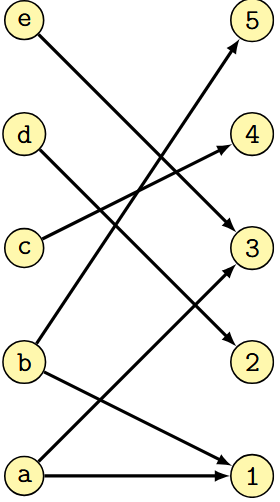
\includegraphics[scale=0.55]{16/graphBipartito.png}
            \caption{Esempio di grafo bipartito}
        \end{subfigure}
        \begin{subfigure}{0.45\textwidth}
            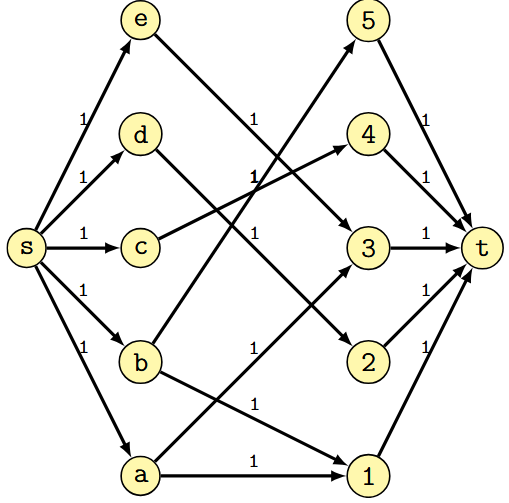
\includegraphics[width=\textwidth]{16/flussoGraphBipartito.png}
            \caption{Esempio di grafo bipartito tradotto in rete di flusso}
        \end{subfigure}
        \caption{Esempio di traduzione da grafo bipartito a rete di flusso}
    \end{figure}
    \chapter{Algoritmi Probabilistici}

Il calcolo delle probabilità applicato alla teoria degli algoritmi è un argomento di grande interesse, in quanto permette di analizzare e progettare algoritmi che si comportano in modo efficiente nella maggior parte dei casi, anche se non garantiscono prestazioni ottimali in tutti i casi. Il calcolo delle probabilità non viene applicato all'input dell'algoritmo, ma ai dati di output dell'algoritmo stesso. Possiamo suddividere gli algoritmi probabilistici in due categorie principali:
\begin{itemize}
    \item Algoritmi la cui correttezza è probabilistica (Montecarlo)
    \item Algoritmi corretti, il cui tempo di esecuzione è probabilistico (Las Vegas)
\end{itemize}

\section{Algoritmi Montecarlo}
    \subsubsection{Test di primalità}
        Il test di primalità è un algoritmo che verifica se un numero intero è primo o meno. Inoltre se un numero non è primo, l'algoritmo restituisce la fattorizzazione del numero.\newline
        La soluzione più semplice è quella di provare a dividere il numero per tutti i numeri compresi tra 2 e la radice quadrata del numero stesso. Se il numero non è divisibile per nessuno di questi numeri, allora è primo. Tuttavia, questo algoritmo ha una complessità temporale di $O(\sqrt{n})$ e può essere migliorato.\newline
        Il piccolo teorema di Fermat afferma che se $n$ è un numero primo allora
        \begin{align*}
            \forall b,2\leq b < n:\qquad b^{n-1} \mod n = 1
        \end{align*}
        Ma questo non può essere usato da solo perché ci sono numeri composti che soddisfano questa condizione. Ad esempio, 561 è un numero composto che soddisfa la condizione di Fermat per $b=2$. Infatti in caso di risultato venga restituito \textsc{true} non è detto che il numero sia primo, la serie dei numeri di \textit{Carmichael} è un insieme di numeri composti che soddisfano il teorema di Fermat per ogni base $b$ fino a $n-1$.
    \paragraph{Teorena di Miller-Rabin}
        Il teorema di Miller-Rabin è un test di primalità probabilistico che può essere usato per determinare se un numero è primo o composto. Il test si basa sul piccolo teorema di Fermat ed enuncia che se $n$ è un numero primo per ogni $b$ con $2\leq b < n$ valgono contemporaneamente le seguenti condizioni:
        \begin{align*}
            mcd(n,b)=&1\\
            b^m\mod n =& 1 \lor \exists i,0\leq i < v: b^{m\cdot 2^i} \mod n = n-1
        \end{align*}
        Possiamo creare un algoritmo probabilistico che sfrutti la contrapposizione del teorema di Miller-Rabin, se \textbf{esiste} un intero $b$ con $2\leq b < n$ rale che \textbf{almeno una} delle due condizioni non è soddisfatta, allora $n$ è composto. \newline
        Una dimostrazione di Rabin ha provato che se $n$ è composto allora ci sono almeno $\frac34(n-1)$ valori di $b$ che non verificano le condizioni. Quindi un algoritmo che verifica le condizioni per $k$ valori di $b$ ha una probabilità di errore inferiore a $\left(\frac{1}{4}\right)^k$. Viene quindi proposto il seguente algoritmo:
        \begin{algorithm}[H]
            \caption{\Bool \textsc{isPrime}(\Item $n$)}
            \begin{algorithmic}
                \For{$i=1$ \textbf{to} $k$}
                    \State $b = \Call{random}{2,n-1}$
                    \If{$\Call{isComposite}{n,b}$}
                        \State \Return \textbf{false}
                    \EndIf
                \EndFor
                \State \Return \textbf{true}
            \end{algorithmic}
        \end{algorithm}
        La complessità di questa funzione è $O(k\log^2n\log\log n \log \log \log n)$, dove $k$ è il numero di iterazioni. La funzione \textsc{isComposite} verifica se $n$ è composto per un dato valore di $b$. La funzione \textsc{random} genera un numero casuale compreso tra 2 e $n-1$. La funzione \textsc{isPrime} restituisce \textbf{true} se il numero è primo, o non si è riuscito a dimostrare che è composto, altrimenti restituisce \textbf{false}.\newline
        Esistono anche degli algoritmi deterministici per il test di primalità, come l'algoritmo di AKS, che ha una complessità polinomiale $O(\log^{6+\epsilon} n)$, ma rimane comunque più lento rispetto agli algoritmi probabilistici visto che le costanti nascoste sono molto elevate. In diverse situazioni comprese quelle di verifica per le chiavi \texttt{RSA} si preferisce usare un algoritmo probabilistico come quello di Miller-Rabin.
    \subsubsection{Espressione polinomiale nulla}
        Un altro esempio di algoritmo Montecarlo è l'algoritmo per determinare se un polinomio di grado $n$ è identicamente nulla. L'algoritmo deterministico che si basa sulla semplificazione del polinomi ha una complessità molto elevata, quindi si può usare un algoritmo probabilistico che lavora nel seguente modo:
        \begin{itemize}
            \item Si genera una $n$-pla di valori $v_1,v_2,\dots,v_n$ in modo uniforme e casuale
            \item Si calcola $x=p(v_1,v_2,\dots,v_n)$
            \subitem Se $x=0$ allora il polinomio è identicamente nullo
            \subitem Se $x\neq 0$ allora il polinomio non è identicamente nullo
            \item Se ogni $v_i$ è un valore intero compreso tra 1 e $2\cdot d$ e il polinomio è di grado $d$, allora la probabilità che l'algoritmo restituisca un risultato errato non è superiore a $\frac{1}{2}$.
            \item Si ripete il test $k$ volte, in modo da ridurre la probabilità di errore a $\left(\frac{1}{2}\right)^k$.
        \end{itemize}
    \subsubsection{BitSet + Tabelle Hash = Bloom Filters}
        I Bloom Filters sono una struttura dati probabilistica che permette di testare se un elemento appartiene a un insieme. La struttura è composta da un array di bit e da una serie di funzioni hash. Le funzioni hash vengono usate per mappare gli elementi dell'insieme in posizioni dell'array di bit. Dunque si ottiene il vantaggio di una struttura dati dinamica che occupa poco spazio e permette di testare se un elemento appartiene a un insieme in tempo costante. Tuttavia, i Bloom Filters non permettono di eliminare gli elementi dall'insieme, la risposta alla ricerca è probabilistica e non c'è vera e propria memorizzazione.
        \begin{itemize}
            \item insert(\textit{key}): per ogni funzione hash $h_i$ si calcola $h_i(key)$ e si imposta il bit in posizione $h_i(key)$ a 1.
            \item \textbf{boolean} contains(\textit{key}): per ogni funzione hash $h_i$ si calcola $h_i(key)$ e si verifica se il bit in posizione $h_i(key)$ è 1. Se tutti i bit sono 1 allora l'elemento è presente, altrimenti non lo è. 
            \subitem Se l'elemento non è presente, allora la risposta è certa. 
            \subitem Se l'elemento è presente, allora la risposta è probabilistica.
        \end{itemize}
        Sia $\epsilon$ la probabilità di errore, ovvero la probabilità che un elemento non presente venga identificato come presente. I Bloom Filters richiedono $1.44\log_2\left(\frac{1}{\epsilon}\right)$ bit per elemento. La probabilità di errore è legata al numero di funzioni hash $k$ e alla dimensione dell'array $m$. Per un confronto rapido ecco una piccola tabella:
        \begin{table}[H]
            \centering
            \begin{tabular}{|c|c|}
                \hline
                $\epsilon$ & $Bit$\\
                \hline
                $10^{-1}$ & 4.78\\
                $10^{-2}$ & 9.57\\
                $10^{-3}$ & 14.36\\
                $10^{-4}$ & 19.15\\
                \dots & \dots\\
                \hline
            \end{tabular}
        \end{table}
        Questo genere di struttura dati è molto usata in ambito web, ad esempio per il chrome safe browsing, per evitare di visitare siti malevoli. Inoltre è usato anche da Medium per evitare di mostrare articoli già letti, Apache HBase per evitare di ri-leggere dati già letti o anche da Ethereum per trovare rapidamente i log della blockchain.
        \paragraph{Forumule e probabilità}
            Dati $n$ oggetti con $m$ bit e $k$ funzioni hash, la probabilità di errore (falso positivo) è data dalla formula:
            \begin{align*}
                \epsilon = \left(1-e^{\frac{-kn}{m}}\right)^k
            \end{align*}
            Dati $n$ oggetti con $m$ bit il valore ottimale per $k$ è:
            \begin{align*}
                k = \frac{m}{n}\cdot\operatorname{ln}(2)
            \end{align*}
            Dato $n$ oggetti ed una probabilità di errore $\epsilon$ il valore ottimale per $m$ è:
            \begin{align*}
                m = -\frac{n\cdot\operatorname{ln}(\epsilon)}{\operatorname{ln}(2)^2}
            \end{align*}
\section{Algoritmi Las Vegas}
    Una applicazione tipica degli algoritmi Las Vegas è la restituzione della media, varianza e moda di un vettore di dati. Oppure anche dato un vettore contenete $n$ valori interi trovare l'elemento che occuperebbe l'elemento $k$ se il vettore fosse ordinato. Oppure anche il calcolo della mediana di un vettore di dati. 
    \subsubsection{Selezione per piccoli valori di $k$}
        Sfruttiamo la memorizzazione con \textit{heap} per calcolare la selezione di un elemento $k$-esimo. L'algoritmo è molto semplice e si basa sulla costruzione di un \textit{heap} di dimensione $n$ con tutti gli elementi del vettore. Una volta costruito l'\textit{heap} si eseguono $k$ estrazioni, in modo da ottenere il valore $k$-esimo. La complessità dell'algoritmo è $O(n+k\cdot\log(n))$, se $k=O(n/\log n)$ allora la complessità diventa $O(n)$ ma se $k=n/2$ allora non è più possibile usare questo algoritmo. Allora usiamo un approccio simile a quello usato per l'algoritmo di \textit{Quicksort} ma non dobbiamo ordinare il vettore, ma solo trovare il valore $k$-esimo e dunque basta cercare nella partizione del vettore che contiene il valore $k$-esimo. 
        \begin{algorithm}[H]
            \caption{\Item \textsc{selection}(\Item[] $A$, \Int $start$, \Int $end$, \Int $k$)}
            \begin{algorithmic}
                \If{$start = end$}
                    \State \Return $A[start]$
                \Else
                    \State $j = \Call{pivot}{A, start, end}$
                    \State $q = j - start + 1$
                    \If{$k = q$}
                        \State \Return $A[j]$
                    \ElsIf{$k < q$}
                        \State \Return \Call{selection}{A, start, j-1, k}
                    \Else
                        \State \Return \Call{selection}{A, j+1, end, k-q}
                    \EndIf
                \EndIf
            \end{algorithmic}
        \end{algorithm}
        Nel caso pessimo l'algoritmo ha una complessità rappresentata dalla seguente ricorrenza:
        \begin{align*}
            T(n) = \begin{cases}
                1 & n\leq 1 \\
                T(n-1) + n & n > 1
            \end{cases}
        \end{align*}
        Il che ha complessita $O(n^2)$. Tuttavia, nel caso ottimo l'algoritmo ha una complessità rappresentata dalla seguente ricorrenza:
        \begin{align*}
            T(n) = \begin{cases}
                1 & n\leq 1 \\
                T(n/2) + n & n > 1
            \end{cases}
        \end{align*}
        Il che ha complessita $O(n)$. Il caso medio dipende dal valore restituito dalla funzione \textsc{pivot}, infatti se questa restituisce in modo casuale una qualsiasi posizione del vettore, allora
        \begin{align*}
            T(n) =& n + \frac1n\sum_{q=1}^n T(\max\{q-1,n-q\}) &\text{Media su } n \text{ casi}\\
            \leq & n + \frac1n\sum_{q=\left\lfloor \frac{n}2 \right\rfloor}^{n-1} 2T(q)  &\text{per } n>1
        \end{align*}
        Dato che è possibile dimostrare che $T(n) \leq cn$ per $c\geq 6$ e $n\geq 1$, il che implica che $T(n) = O(n)$.\newline
        Dunque partendo dall'assunzione che \textsc{pivot} restituisca un valore casuale, (ed in caso negativo lo sostituiamo con un valore casuale) possiamo affermare che l'algoritmo nel caso medio ha una complessità di $O(n)$ per la selezione e $O(n\log n)$ per l'ordinamento. 
        \paragraph{Selezione deterministica}    
            Supponendo di avere un algoritmo che restituisca al più un valore che disti $\frac{3}{10}n$ dal valore mediano. Allora modifichiamo l'algoritmo di selezione come segue:
            \begin{itemize}
                \item Dividiamo il vettore in $n/5$ sotto-vettori di dimensione 5, ed l'i-esimo sotto-vettore lo chiamiamo $S_i$ con $i\in[1,\left\lceil\frac{n}{5}\right\rceil]$.
                \item Calcoliamo il valore mediano di ogni sotto-vettore $S_i$ e calcoliamo il valore mediano $m$ dei valori mediani.
                \item Usiamo $m$ come pivot e eseguiamo chiamate ricorsive come per la \textsc{selection}
                \item Se la dimensione scende sotto 10, allora ordiniamo il sotto-vettore e restituiamo il valore mediano che sarà il valore $k$-esimo.
            \end{itemize}
            \begin{algorithm}[H]
                \caption{\Item \textsc{select}(\Item[] $A$, \Int $start$, \Int $end$, \Int $k$)}
                \begin{algorithmic}
                    \If{$end - start + 1 \leq 10$}
                        \State \Call{insertionSort}{A, start, end}
                        \State \Return $A[start + k - 1]$
                    \EndIf
                    \State $m = \New\Int[1,\left\lceil\frac{end-start+1}{5}\right\rceil]$
                    \For{$i=0$ \textbf{to} $\left\lceil\frac{end-start+1}{5}\right\rceil$}
                        \State $m[i] = \Call{median}{A, start + 5i, start + 5i + 4}$
                    \EndFor
                    \State \Item $ m \gets \Call{select}{m, 1, \left\lceil\frac{end-start+1}{5}\right\rceil, \left\lceil\frac{\left\lceil\frac{end-start+1}{5}\right\rceil}{2}\right\rceil}$
                    \State \Int $j = \Call{pivot}{A, start, end, m}$
                    \State \Int $q = j - start + 1$
                    \If{$k = q$}
                        \State \Return $m$
                    \ElsIf{$k < q$}
                        \State \Return \Call{select}{A, start, j-1, k}
                    \Else
                        \State \Return \Call{select}{A, j+1, end, k-q}
                    \EndIf
                \end{algorithmic}
            \end{algorithm}
            Come dimostrato il calcolo dei mediani $M[]$ richiede al più $6\left\lceil\frac{n}{5}\right\rceil$ confronti, e la chiamata ricorsiva della funzione \textsc{select} viene eseguita su sotto-vettori di al più $\left\lceil\frac{n}{5}\right\rceil$ elementi. La seconda chiamata ricorsiva viene eseguita su un sotto-vettore di dimensione al più $\frac{7}{10}n$ e infine nel caso pessimo l'algoritmo la complessità è $O(n)$ ma nel caso medio è $T(n)=t(\frac{n}{5})+T(\frac{7n}{10})+\frac{11}{5}n$, il che implica che la complessità è $O(n)$.
\end{document}